\chapter{Complex Analysis}
\section{The Cauchy theory}
\subsection{Integration of differential forms}
\subsubsection{Integration on piecewise differentiable paths; exact and closed forms}
\begin{definition}
Let $D$ be a domain in $\C$. A differential form $\omega$ on $D$ is an expression
\[\omega=P\dif x+Q\dif y\]
where $P=P(x,y)$ and $Q=Q(x,y)$ are continuous (complex-valued) functions on $D$. We say $\omega$ is a \textbf{$\bm{C^p}$ form} if $P$ and $Q$ are of class $C^p$.\par
If $\gamma$ is a differentiable path in $D$ and $\omega$ is a differential form on $D$, then we define the line integral of $\omega$ along $\gamma$ by the formula
\begin{align*}
\int_{\gamma}\omega&=\int_{a}^{b}[P(x(t),y(t))x'(t)+Q(x(t),y(t))y'(t)]\dif t.
\end{align*}
where the integral is computed by real and imagary parts separately.
\end{definition}
The definition above is just an variant of line integrals of real differential forms, and many analogues hold in this case. For example, if $\varphi:[c,d]\to[a,b]$ is an increasing diffeomorphism, then
\[\int_{\gamma}\omega=\int_{\widetilde{\gamma}}\omega\]
where $\widetilde{\gamma}:=\gamma\circ\varphi$.\par
Now let $D$ be a domain in $\C$. By a \textbf{curve segment} in $D$ we mean a continuous curve $\gamma:[a,b]\to D$ whose domain is a compact interval. It is a smooth curve segment if it is smooth when $[a,b]$ is considered as a manifold with boundary. It is a \textbf{piecewise differentiable} if there exists a finite partition 
\[a=a_0<a_1<\cdots<a_k=b\]
such that $\gamma|_{[a_{i-1},a_i]}$ is smooth for each $i$. For a piecewise differentiable path, we define the integral of $\omega$ on $\gamma$ by
\[\int_{\gamma}\omega:=\sum_{i=1}^{n}\int_{\gamma_i}\omega.\]
It is easy to see the path integral over a piecewise differentiable path is well defined (independent of the partition) and agrees with our earlier definition for differentiable paths.
\begin{definition}
Let $\gamma$ denote a piecewise differentiable path parameterized by $[a,b]$ in a domain $D$. Then
the path $\gamma$ traversed backward is defined by
\[\widebar{\gamma}(t):=\gamma(a+b-t)\]
for $t\in[a,b]$. It follows that
\[\int_{\widebar{\gamma}}\omega=-\int_{\gamma}\omega.\]
\end{definition}
\begin{definition}
If $\gamma_1$ and $\gamma_2$ are piecewise differentiable paths in $D$ parameterized by $[0,1]$, with $\gamma_1(1)=\gamma_2(0)$, then a new piecewise differentiable path $\gamma_1\ast\gamma_2$ in $D$ may be defined by first traversing $\gamma_1$ and then continuing with $\gamma_2$, as follows:
\[(\gamma_1\ast\gamma_2)(t)=\begin{cases}
\gamma_1(2t)&t\in[0,1/2],\\
\gamma_2(2t-1)&t\in[1/2,1].
\end{cases}\]
It follows that
\[\int_{\gamma_1\ast\gamma_2}\omega=\int_{\gamma_1}\omega+\int_{\gamma_2}\omega.\]
for all differential forms $\omega$ defined in a neighborhood of the range of $\gamma_1\ast\gamma_2$.
\end{definition}
\begin{proposition}
If $D$ is a domain in $\C$, then any two points in $D$ can be joined by a
piecewise differentiable path in $D$.
\end{proposition}
\begin{proof}
This follows from the connectedness of $D$.
\end{proof}
For a given function $f$, we have the (real) partial derivatives $f_x$ and $f_y$ as well as the formal (complex) partial derivatives $\partial f/\partial z$ and $\partial f/\partial\widebar{z}$ defined by
\[\frac{\partial f}{\partial z}=\frac{1}{2}\Big(\frac{\partial f}{\partial x}-i\frac{\partial f}{\partial y}\Big),\quad \frac{\partial f}{\partial\widebar{z}}=\frac{1}{2}\Big(\frac{\partial f}{\partial x}+i\frac{\partial f}{\partial y}\Big).\]
Similarly, we consider the differentials
\[\dif z=\dif x+i\dif y,\quad \dif\widebar{z}=\dif x-i\dif y.\]
It follows that every differential form can be written in the following two ways:
\[P\dif x+Q\dif y=\frac{1}{2}(P-iQ)\dif z+\frac{1}{2}(P+iQ)\dif\widebar{z}.\]
If $f$ is a $C^1$-function on $D$, then we define $df$, the total differential of $f$, by either of the two equivalent formulas:
\[df=f_x\dif x+f_y\dif y=f_z\dif z+f_{\widebar{z}}\dif\widebar{z}.\]
In addition to the differential operator $d$, we have two other important differential operators $\partial$ and $\widebar{\partial}$ defined by
\[\partial f=f_z\dif z,\quad\widebar{\partial}f=f_{\widebar{z}}\dif\widebar{z}.\]
as well as the formula
\[d=\partial+\widebar{\partial}.\]
Similar to the real case, a differential form $\omega$ is called \textbf{exact} if there exists a $C^1$-function $F$ on $D$ (called a \textbf{primitive} for $\omega$) such that $\omega=dF$. A primitive (if it exists) is unique up to addition of a constant, because $dF=0$ means $F_x=F_y=0$, and this implies that $F$ is constant on the connected set $D$.\par
A differential form $\omega$ on $D$ is \textbf{closed} if it is locally exact; that is, if for each $z\in D$ there exists a neighborhood $U$ of $z$ in $D$ such that $\omega|_U$ is exact. After we introduce the differential of a one form, this condition will have a easy justification.\par
To understand the difference of exact forms and closed forms, we study the pairing that associates the complex number
\[\langle\gamma,\omega\rangle=\int_{\gamma}\omega\]
to a piecewise differentiable path $\gamma$ in a domain $D$ and a differential form $\omega$ on $D$.
\begin{proposition}[\textbf{Characterization of exact forms}]\label{complex form exact iff}
Let $\omega$ be a differential form on a domain $D$. Then $\omega$ is exact on $D$ if and only if $\int_{\gamma}\omega=0$ for all closed piecewise differentiable paths $\gamma$ in $D$.
\end{proposition}
\begin{proof}
Assume that $\omega$ is exact. Then there exists a $C^1$-function $F$ on $D$ with
\[\omega=F_x\dif x+F_y\dif y\]
If $\gamma$ is a piecewise differentiable path parameterized by $[a,b]$ joining two points $z_1$ to $z_2$ in $D$, then
\[\int_{\gamma}\omega=\int_{a}^{b}\Big(F_x\frac{\dif x}{\dif t}+F_y\frac{\dif x}{\dif y}\Big)\dif t=\int_{a}^{b}\frac{dF}{\dif t}\dif t=F(z_2)-F(z_1).\]
which equals zero if $P_1=P_2$, as happens for every closed curve. To prove the converse, let $(x_0,y_0)$ be a fixed point in $D$ and let $(x,y)$ be an arbitrary point in $D$. Let $\gamma$ be a piecewise differentiable path in $D$ joining $z_0$ to $z$ and define
\[F(x,y)=\int_{\gamma}\omega.\]
To see that the function $F$ is well defined on $D$, note that if $\gamma_2$ is another piecewise differentiable path in $D$ joining $z_0$ to $z$, then $\gamma_1\ast\widebar{\gamma}_2$ is a closed piecewise differentiable path in $D$, and it follows from the hypothesis that
\[0=\int_{\gamma_1\ast\widebar{\gamma}_2}=\int_{\gamma_1}\omega-\int_{\gamma_2}\omega.\]
We must show that $F\in C^1(D)$ and $dF=\omega$. Choose $\eps>0$ so that $U:=B_{\eps}(x,y)\sub D$ also choose $x_1\neq x$ such that $(x_1,y)\in U$ and the (straight) segment $L$ from $(x_1,y)$ to $(x,y)$ is contained in $D$. Let $\gamma'$ be any piecewise differentiable path in $D$ from $(x_0,y_0)$ to $(x_1,y)$, and assume that $\omega=P\dif x+Qsy$. Then
\[F(X,y)=\int_{\gamma'}\omega+\int_{x_1}^{x}P(t,y)\dif t\]
It is now clear that $F_x=P$. Similarly $F_y=Q$.
\end{proof}
For future use it is important to record the following result.
\begin{corollary}
If $\omega=dF$ is an exact differential form on the domain $D$ and $\gamma$ is a piecewise differentiable path in $D$ starting at $z_1$ and ending at $z_2$, then
\[\int_{\gamma}\omega=F(z_2)-F(z_1).\]
\end{corollary}
\begin{theorem}[\textbf{Exact forms on an open disk}]\label{complex form exact on disk iff}
Let $\omega$ be a differential form on an open disc $U$. Then $\omega$ is exact on $U$ if and only if $\int_{\gamma}\omega=0$ for all $\gamma$ that are boundaries of rectangles contained in $U$ with sides parallel to the coordinate axes.
\end{theorem}
\begin{proof}
Repeat the argument in the proof of Proposition~\ref{complex form exact iff} with $(x_0,y_0)$ the center of $U$, observing that any other point in the disc may be joined to the center by either a vertical segment, a horizontal segment, or two consecutive segments, one horizontal and one vertical.
\end{proof}
Using Theorem~\ref{complex form exact on disk iff}, we can now characterize closed forms and exact forms on an open disk in $\C$. It turns out that they are the same.
\begin{proposition}\label{complex form closed on disk iff exact}
A differential form $\omega$ is closed on an open disc if and only if it is exact on the disc.
\end{proposition}
\begin{proof}
Every exact form on a domain is closed, so we just need to show that the converse holds on an open disc. So assume $\omega$ is a closed form on the open disc $U$. By the theorem, it is enough to show that if $R$ is any rectangle contained in $U$, with sides parallel to the coordinate axes, then $\int_{\partial R}\omega=0$. Note that the rectangle $R$ may be subdivided into smaller rectangles with sides parallel to the coordinate axes and such that each smaller rectangle is contained in an open set in $U$ where $\omega$ is exact. It follows from the theorem that the integral of $\omega$ over the boundary of each smaller rectangle is equal to zero, and therefore the integral of $\omega$ over the boundary of $R$, being equal to the sum of all the integrals over the boundaries of the smaller rectangles, is also equal to zero.
\end{proof}
\begin{corollary}\label{complex form closed iff}
If $\omega$ is a differential form on a domain $D$, then $\omega$ is closed on $D$ if and only if $\int_{\gamma}\omega=0$ for all curves $\gamma$ that are boundaries of rectangles contained in $D$ with sides parallel to the coordinate axes.
\end{corollary}
We recall and establish a form of a theorem that will help us to further distinguish closed from exact differentials.
\begin{theorem}[\textbf{Green's Theorem}]
Let $K$ be a compact set in $\C$ which is the closure of its interior, with piecewise smooth positively oriented boundary $\partial K$. If $P$ and $Q$ are $C^1$-functions on a neighborhood of $K$, then
\[\iint_{K}\Big(\frac{\partial Q}{\partial x}-\frac{\partial Q}{\partial y}\Big)\mathrm{d}x\mathrm{d}y=\int_{\partial K}P\dif x+Q\dif y.\]
In terms of complex derivatives, the can be restated as
\[\iint_{K}\Big(\frac{\partial Q}{\partial z}-\frac{\partial Q}{\partial\widebar{z}}\Big)\mathrm{d}z\mathrm{d}\widebar{z}=\int_{\partial K}P\dif z+Q\dif\widebar{z}.\]
where $\dif z\dif\widebar{z}=-2i\dif x\dif y$.
\end{theorem}
We can now characterize the closed $C^1$-forms.
\begin{theorem}[\textbf{Characterization of closed forms}]\label{complex form closed derivative char}
Let $D$ be a domain. A $C^1$-differential form $\omega=P\dif x+Q\dif y$ on $D$ is closed if and only if $P_y=Q_x$ in $D$, and a $C^1$-differential form $\omega=P\dif z+Q\dif\widebar{z}$ on $D$ is closed if and only if $P_{\widebar{z}}=Q_z$ in $D$.
\end{theorem}
\begin{proof}
We only prove the case $\omega=P\dif x+Q\dif y$, the complex notation can be done similarly. If $\omega$ is closed in the domain $D$, then near every point in $D$ there exists a function $F$ such that $\omega=F_x\dif y+F_y\dif y$. But $\omega$ is $C^1$ and thus $F$ is $C^2$; therefore $P_y=F_{xy}=F_{yx}=Q_x$.\par
For the converse, since by Corollary~\ref{complex form closed iff}, we need only show that $\int_{\gamma}\omega=0$ for all paths $\gamma$ in $D$ that are boundaries of rectangles $R$ with sides parallel to the coordinate axes and such that $\widebar{R}\sub D$. But
\[\int_{\gamma}\omega=\iint_{R}(Q_x-P_y)\dif x\dif y=0.\]
Therefore the claim follows.
\end{proof}
\begin{remark}
Recall that if $f=u+iv$, then
\[f(z)\dif z=(u+iv)(\dif x+i\,\dif y)=(u\,\dif x-v\,\dif y)+i(v\,\dif x+u\,\dif y).\]
Further, $f(z)\dif z$ is closed (respectively exact) if and only if both $\omega_1$ and $\omega_2$ are, and $F_i$ is a primitive for $\omega_i$ ($i=1,2$) if and only if $F_1+iF_2$ is a primitive for $f(z)\dif z$.
\end{remark}
Now we relate the concept of closed and exact forms with holomorphic function. The following result is our first important observation.
\begin{proposition}
Let $f(z)\dif z$ be of class $C^1$ on a domain $D$. Then $f(z)\dif z$ is closed on
$D$ if and only if $f$ is holomorphic in $D$.
\end{proposition}
\begin{proof}
By the above remarks and previous Theorem, $f(z)\dif z$ is a closed form on $D$ if and only if $u_x=v_y$ and $v_y=-u_x$ if and only if $u$ and $v$ satisfy $CR$-equation, if and only if $f$ is holomorphic.
\end{proof}
\begin{proposition}
A $C^1$-function $F$ is a primitive for $f(z)\dif z$ if and only if $F'=f$.
\end{proposition}
\begin{proof}
The function $F$ is a primitive for $f(z)\dif z$ if and only if $dF=F_z\dif z+F_{\widebar{z}}\dif\widebar{z}=f(z)\dif z$, if and only if $F_{\widebar{z}}=0$ and $F_z=F'=f$.
\end{proof}
We have now proven the following result that gives a preliminary characterization of certain closed forms.
\begin{theorem}
The differential form $f(z)\dif z$ is closed on a domain $D$ if and only
if $\int_{\gamma}f(z)\dif z=0$, for all boundaries $\gamma$ of rectangles $R$ contained in $D$ with sides parallel to the coordinate axes. If $f\in C^1(D)$, then $f(z)\dif z$ is closed if and only if $f$ is holomorphic on $D$.
\end{theorem}
\begin{example}\label{complex form closed no exact eg}
Not every closed form is exact. Let $D=\C^*$ and $\omega=\dif z/z$. Then
\[\int_{|z|=1}\omega=\int_{0}^{2\pi}\frac{ie^{i\theta}\dif \theta}{e^{i\theta}}=2\pi i.\]
Thus $\omega$ is not exact in $D$. However, since $1/z$ is holomorphic and $C^1$ on $D$, $\omega$ is closed on $D$. Note that locally (in $D$) we have $\omega=dF$, where $F$ is a branch of the logarithm, and that we have just proved that there is no branch of the logarithm globally defined on $D$.\par
We have produced two real forms on $D=\C^*$, the real and imaginary parts of $\omega$:
\[\omega=\frac{x\dif x+y\dif y}{x^2+y^2}+i\frac{-y\dif x+x\dif y}{x^2+y^2}=\dif\log|z|+i\dif\arg z=\dif\log z.\]
The first of the two real forms is exact, the second closed but not exact on $D$. Note that $\dif\arg z=\dif\arctan(y/x)$ (for $x\neq 0$). Note also that $\arg z$ and $\arctan(y/x)$ are multivalued functions, whose differentials agree and are single-valued. It is important to observe that if we change the domain $D$ then $\omega$ may become exact; for instance, on the domain $\C\setminus[0,+\infty]$ the same form $\omega=\dif z/z$ is exact because $\dif\Log z$, where $\Log z$ denotes the principal branch of the  ogarithm in this domain.
\end{example}
To place the discussion of differential forms in its broader context, we outline some basic concepts of the exterior differential calculus for domains $D\sub\C$ using only complex coordinates $z=x+iy$. For every nonnegative integer $n$, let $\Omega^n(D)$ denote the space of $n$-forms on $D$. Since $D$ is two dimensional over the reals, we need to consider only $n=0,1,2$.\par
The set $\Omega^0(D)$ consists of smooth functions on $D$. The space $\Omega^1(D)$ can be viewed as a module over $\Omega^0(D)$ generated by the $1$-forms $dz$ and $d\widebar{z}$; that is, expressions of the form $f(z)\dif z+g(z)\dif\widebar{z}$ with $f$ and $g$ smooth, subject however to the appropriate transformation rule under complex coordinate changes ($w$ is an injective holomorphic function of $z$):
\[F(w)\dif w+G(w)\dif\widebar{z}=F(w(z))w'(z)\dif z+G(w(z))\widebar{w'(z)}\dif\widebar{z}.\]
and the general rule about exterior multiplication $\wedge$ of forms is given as follows:
\[\dif z\wedge \dif z=\dif\widebar{z}\wedge\dif\widebar{z}=0,\quad \dif  z\wedge \dif\widebar{z}=-\dif\widebar{z}\wedge \dif z=-2i\dif x\wedge\dif y.\]
The set $\Omega^2(D)$ consists of elements of the form
\[f(z)\dif z\wedge\dif\widebar{z}=F(w)\dif w\wedge \dif\widebar{w}\]
where $f$ and $F$ are $C^\infty$-functions with
\[f(z)=F(w(z))|w'(z)|^2.\]
where $w$ is an injective holomorphic function of $z$.\par
The space of one-forms $\Omega^1(D)$ decomposes as a direct sum
\[\Omega^1(D)=\Omega^{(1,0)}(D)\oplus\Omega^{(0,1)}(D)\]
where
\[\Omega^{(1,0)}(D)=\{\omega\in\Omega^1(D):\omega=f(z)\dif z\},\quad \Omega^{(0,1)}(D)=\{\omega\in\Omega^1(D):\omega=f(z)\dif\widebar{z}\}.\]
Three differential operators, $\partial$, $\widebar{\partial}$, and $d=\partial+\widebar{\partial}$ act on forms; each of these follows the product rule; for example,
\[d(\omega_1\wedge\omega_2)=d\omega_1\wedge\omega_2+\omega_1\wedge d\omega_2.\]
Thus these operators are completely determined by their actions on functions (of $z$) and the distinguished one forms $\dif z$ and $\dif\widebar{z}$, for example
\[\partial(f(z))=f_z\dif z,\quad \partial(\dif z)=\partial(\dif\widebar{z})=0,\]
and
\[\widebar{\partial}(f(z))=f_{\widebar{z}}\dif\widebar{z},\quad \widebar{\partial}(\dif z)=\widebar{\partial}(\dif\widebar{z})=0.\]
One can easily check that
\[0=\partial^2=\partial\widebar{\partial}+\widebar{\partial}\partial=\widebar{\partial}^2,\quad d^2=\partial\widebar{\partial}+\widebar{\partial}\partial=0.\]
The differential operators lead to the following diagram
\[\begin{tikzcd}
\Omega^{(0,1)}(D)\ar[r,"\partial"]&\Omega^2(D)\\
\Omega^0(D)\ar[r,"\partial"]\ar[u,"\widebar{\partial}"]&\Omega^{(1,0)}(D)\ar[u,swap,"\widebar{\partial}"]
\end{tikzcd}\]
Note that in this langudge, a one form $\omega\in\Omega^1(D)$ is closed if and only if $d\omega=0$, and is exact if and only if $\omega=dF$ for some $F\in\Omega^0(D)$. 
\subsubsection{Integration of closed forms and the winding number}
We have been working with the integral of any differential form over any piecewise differentiable path. We want to extend the definition to the integral over any continuous path $\gamma$ but only for closed differential forms. The next result will lead us in that direction.
\begin{definition}
Let $D$ be a domain in $\C$, $\gamma:[a,b]\to D$ be a continuous path in $D$, and $\omega$ be a closed form in $D$. A \textbf{primitive for $\omega$ along $\gamma$} is a continuous function $f:[a,b]\to\C$ such that for all $t_0\in[a,b]$ there exists a neighborhood $N$ of $\gamma(t_0)$ in $D$ and a primitive $F$ for $\gamma$ in $N$ such that $F(\gamma(t))=f(t)$ for all $t$ in a neighborhood of $t_0$ in $[a,b]$.
\end{definition}
\begin{theorem}\label{complex form primitive along curve exist unique}
If $\gamma$ is a continuous path in a domain $D$ and $\omega$ is a closed form on $D$, then there exists a primitive $f$ of $\omega$ along $\gamma$. Furthermore, $f$ is unique up to the addition of a constant.
\end{theorem}
\begin{proof}
Suppose $\gamma$ is parameterized by $[a,b]$ and $\omega=P\dif x+Q\dif y$. Suppose $f$ and $g$ are two primitives of $\omega$ along $\gamma$ and let $t_0\in[a,b]$. Then there exist primitives $F$ and $G$ of $\omega$ in a connected neighborhood $U$ of $\gamma(t_0)$ in $D$ such that
\[F(\gamma(t))=f(t),\quad G(\gamma(t))=g(t).\]
for $t$ near $t_0$. Hence $F_x=G_x=P$ and $F_y=G_y=Q$ in $U$; thus $F-G$ is constant in $U$, and therefore $f-g$ is constant near $t_0$. We conclude that $f-g$ is a continuous and locally constant function on the connected set $[a,b]$, and thus $f-g$ is a constant function.\par
Now we construct a primitive for $\omega$ along $\gamma$. Given $t\in[a,b]$, there exists an interval $I(t)\sub[a,b]$ (open in $[a,b]$ and containing $t$) and an open set $U(\gamma(t))\sub D$ such that $\omega$ has a primitive in $U(\gamma(t))$ and $\gamma(I(t))\sub U(\gamma(t))$. Then $\{I(t):t\in[a,b]\}$ is an open cover of $[a,b]$ and thus there exists a finite subcover
\[I_0\cup I_1\cup\cdots I_n=[a,b].\]
with corresponding $U_i$. Without loss of generality we may assume $I_i=[a_i,b_i)$ for $i=0,\dots,n$, where
\[a=a_0<b_0<a_1<b_1<\cdots<a_{n-1}<b_{n-1}<a_n<b_n=b.\]
Further, $\gamma(I_i)\sub U_i$ and $\omega$ has a primitive $F_i$ on $U_i$ for $i=0,\dots,n$. Set $f(t)=F_0(\gamma(t))$ for $t\in I_0$. Having defined $f$ on $I_0\cup\cdots\cup I_k$ for $0\leq k<n$, we define $f$ on $I_{k+1}$ as follows. Let $F_{k+1}$ be any primitive for $\omega$ in $U_{k+1}$ and let $F_k$ be the primitive for $\omega$ in $U_k$ such that $f(t)=F_k(\gamma(t))$ for $t\in I_k$. Then $F_{k+1}$ and $F_k$ are two primitives for $\omega$ in $U_{k+1}\cap U_k$, and thus $F_{k+1}-F_k$ is constant on each connected component of $U_{k+1}\cap U_k$; in particular, let $F_{k+1}-F_{k}=c$ on the component containing $\gamma(I_{k+1}\cap I_k)$. Set $f(t)=F_{k+1}(\gamma(t))-c$ for $t\in I_{k+1}$, then $f$ is well defined on $I_{k+1}\cap I_k$.
\end{proof}
We use Theorem~\ref{complex form primitive along curve exist unique} to compute $\int_{\gamma}\omega$, where $\omega$ is a closed differential form in $D$ and $\gamma:[a,b]\to D$ is a piecewise differentiable path in $D$.\par
Subdivide $[a,b]=I_0\cup\cdots\cup I_n$, where $I_i=[a_i,b_i]$, such that $\gamma_i:=\gamma|_{I_i}$ is a differentiable path and $\omega$ has a primitive $F_i$ in a neighborhood of $\gamma(I_i)$ for $i=0,\dots,n$. By the theorem, there exists a primitive $f$ of $\omega$ along $\gamma$. Then
\[\int_{\gamma}\omega=\sum_{i=0}^{n}\int_{\gamma_i}\omega=\sum_{i=0}^{n}\int_{\gamma_i}\dif F_i=f(b)-f(a).\]
Using this equation, we extend the concept of a line integral to continuous paths.
\begin{definition}
Let $\omega$ be a closed differential form in $D$ and $\gamma:[a,b]\to D$ be a continuous path in $D$. We define the \textbf{integral of $\bm{\omega}$ along $\bm{\gamma}$} by
\[\int_{\gamma}\omega:=f(b)-f(a)\]
where $f$ is a primitive of $\omega$ along $\gamma$.
\end{definition}
An important example of this definition, which will be used later, is the winding number of a continuous path.
\begin{definition}
Let $z\in\C$ and let $\gamma$ be a continuous closed path in $\C\setminus\{z\}$. We define the \textbf{index} or \textbf{winding number} of $\gamma$ with respect to $z$ as the following number:
\[I(\gamma,z):=\frac{1}{2\pi i}\int_{\gamma}\frac{\dif\zeta}{\zeta-z}\]
\end{definition}
\begin{proposition}
For every $z\in\C$ and every continuous closed path $\gamma$ in $\C\setminus\{z_0\}$, the number
\[\frac{1}{2\pi i}\int_{\gamma}\frac{\dif z}{z-z_0}\]
is an integer.
\end{proposition}
\begin{proof}
We may assume $z_0=0$. Let $f$ be a primitive of $\dif z/z$ along the curve $\gamma$. Then
\[\int_{\gamma}\frac{\dif z}{z}=f(b)-f(a)\]
where $[a,b]$ parameterizes $\gamma$. Since $\gamma(a)=\gamma(b)$, we know from Example~\ref{complex form closed no exact eg} that $f(b)-f(a)$ is just the difference between two branches of $\log z$ at the same point, hence of the form $2\pi in$ with $n$ in $\Z$.
\end{proof}
\begin{example}
Let $r=f(\theta)>0$, with $f\in C^1(\R)$. Let $n\in\Z$ be a positive integer and define $\gamma(\theta)=f(\theta)e^{i\theta}$, where $\theta\in[0,2\pi n]$. Assume that $f(0)=f(2\pi n)$. Observe that the conditions on $f$ imply that the curve $\gamma$ winds around the origin $n$ times in the counterclockwise direction and, as expected,
\begin{align*}
I(\gamma,0)&=\frac{1}{2\pi i}\int_{\gamma}\frac{\dif z}{z}=\frac{1}{2\pi i}\int_{0}^{2\pi n}\frac{f'(\theta)e^{i\theta}+if(\theta)e^{i\theta}}{f(\theta)e^{i\theta}}\dif\theta\\
&=\frac{1}{2\pi i}\int_{0}^{2\pi n}\Big[\frac{f'(\theta)}{f(\theta)}+i\Big]\dif \theta=n.
\end{align*}
\end{example}
In general, let $\gamma:[a,b]\to\C\setminus\{z_0\}$ be a continuous closed path and let $f$ be a primitive of $\dif z/(z-z_0)$ on $\gamma$. Then $f(t)$ agrees with a branch of $\log(\gamma(t)-z_0)$; that is
\[e^{f(t)}=\gamma(t)-z_0\for t\in[a,b].\]
Hence
\[I(\gamma,z_0)=\frac{f(b)-f(a)}{2\pi i}.\]
We see that the $C^1$ assumption on $f$ is unnecessary as we will also be able to conclude using homotopy of curves discussed in the next part.
\subsubsection{Homotopy and simple connectivity}
In order to give the integration results the clearest formulation, we need the topological concepts of homotopic curves and simply connected domains. Let's recall the following definitions.
\begin{definition}
Let $\gamma_0$ and $\gamma_1$ be two continuous paths in a domain $D$, parameterized by $I=[0,1]$ with the same end points; that is, $\gamma_0(0)=\gamma_1(0)$ and $\gamma_0(1)=\gamma_1(1)$. We say that $\gamma_0$ and $\gamma_1$ are \textbf{homotopic on $\bm{D}$ (with fixed end points)} if there exists a continuous function $H:I\times I\to D$ such that
\begin{itemize}
\item $H(t,0)=\gamma_0(t)$.
\item $H(t,1)=\gamma_1(t)$.
\item $H(0,s)=\gamma_0(0)=\gamma_1(0)$.
\item $H(1,s)=\gamma_0(1)=\gamma_1(1)$.
\end{itemize}
We call $H$ a homotopy with fixed end points between $\gamma_0$ and $\gamma_1$, with $\gamma_s(t)=H(t,s)$ for fixed $s$ in $I$.\par
Let $\gamma_0$ and $\gamma_1$ be two continuous closed paths in a domain $D$ parameterized by $[0,1]$. We say that $\gamma_0$ and $\gamma_1$ are \textbf{homotopic as closed paths} on $D$ if there exists a continuous function $H:I\times I\to D$ such that
\begin{itemize}
\item $H(t,0)=\gamma_0(t)$.
\item $H(t,1)=\gamma_1(t)$.
\item $H(0,s)=H(1,s)$.
\end{itemize}
The map $H$ is called a \textbf{homotopy of closed paths}, with $\gamma_s(t)=H(t,s)$ for fixed $s$ in $I$.\par
Finally, a continuous closed path is \textbf{null-homotopic} if it is homotopic to a constant path as a closed path. 
\end{definition}
\begin{remark}
Note that in our definitoin of homotopic closed paths, we allow the end point to move in the homotopy. This is often called \textbf{free homotopy}. If we do not allow $\gamma_0(0)$ and $\gamma_1(0)$ to move during the homotopy, then we get stronger condition on homotopic of closed paths. As we will see, these two definitions have no effect on our main result, but the first one is much convenient in applications.
\end{remark}
Note that the notion of being homotopic depends on the domain $D$. For instance, the closed path $\gamma(t)=e^{it}$ is null-homotopic in $\C$, but it is not null-homotopic in $\C\setminus\{0\}$, as we will soon see.
\begin{definition}
Let $D$ be a domain in $\C$ and $H:I\times I\to D$ be a continuous map, and
let $\omega$ be a closed form on $D$. A function $f:I\times I\to\C$ is said to be a primitive for $\omega$ along $H$ provided for every $(t_0,s_0)\in I\times I$, there exists a neighborhood $V$ of $H(t_0,s_0)$ in $D$ and a
primitive $F$ for $\omega$ on $V$ such that
\[f(t,s)=F(H(t,s))\]
for all $(t,s)$ in a neighborhood of $(t_0,s_0)$ in $I\times I$.
\end{definition}
It is easy to see that if $f$ is a primitive of $\omega$ along $H$, then for fixed $s\in I$, $f(\cdot,s)$ is a primitive for $\omega$ along the path $\gamma_s$.
\begin{theorem}
If $\omega$ is a closed form on $D$ and $H:I\times I\to D$ is a continuous map, then a primitive $f$ for $\omega$ along $H$ exists and is unique up to an additive constant.
\end{theorem}
\begin{proof}
This is proved as in Theorem~\ref{complex form primitive along curve exist unique}, but by subdividing $I\times I$ by small squres.
\end{proof}
We now observe that all integrals of a closed form along homotopic paths coincide.
\begin{theorem}\label{complex form integral homotopy}
Let $\gamma_0$ and $\gamma_1$ be continuous paths in a domain $D$ and let $\omega$ be a closed form on $D$. If $\gamma_0$ is homotopic to $\gamma_1$ with fixed end points (or closed paths, if they are both closed), then
\[\int_{\gamma_0}\omega=\int_{\gamma_1}\omega.\]
\end{theorem}
\begin{proof}
We assume that both paths are parameterized by the interval $I=[0,1]$. Let $H:I\times I\to D$ be a homotopy between our two paths and let $f$ be a primitive of $\omega$ along $H$. Then as we have mentioned, $f(0,s)$ and $f(1,s)$ are both primitives of $\omega$ along the path $t\mapsto\gamma(0,t)=\gamma(1,t)$, so they differ by a constant. From the observation
\[\int_{\gamma_0}\omega=f(1,0)-f(0,0),\quad\int_{\gamma_1}\omega=f(1,1)-f(0,1)\]
we see that $\int_{\gamma_0}\omega=\int_{\gamma_1}\omega$, and the theorem is proved.
\end{proof}
\begin{corollary}
If $\gamma$ is null-homotopic in $D$ and $\omega$ is a closed form in $D$, then
\[\int_{\gamma}\omega=0.\]
\end{corollary}
This corollary motivates the following.
\begin{definition}
A domain $D\sub\C$ is called \textbf{simply connected} if every continuous closed path in $D$ is null-homotopic in $D$.
\end{definition}
\begin{corollary}
If $D$ is a simply connected domain and $\gamma$ is a continuous closed path in $D$, then $\int_{\gamma}\omega=0$ for all closed forms $\omega$ on $D$.
\end{corollary}
With these praperations, we obtain the simplest formulation of the main result:
\begin{corollary}
In a simply connected domain a differential form is closed if and only if it is exact.
\end{corollary}
An immediate corollary gives the existence of branches of the logarithm:
\begin{proposition}
In every simply connected domain not containing the point $0$, there exists a branch of $\log z$.
\end{proposition}
\begin{proof}
The differential form $\omega=\dif z/z$ is closed and thus exact in the given domain. Hence there exists a holomorphic function $F$ (on the same domain) such that $dF=\omega$. This function $F$ is a branch of the logarithm.
\end{proof}
\subsubsection{More on the winding number}
We defined the winding number $I(\gamma,z_0)$ of a curve $\gamma$ with respect to a point $z_0$ not on its range. In this section we will see that arguments involving the winding number allow us to draw strong conclusions about the behavior of a function defined in a disc.
We begin with some properties of $I(\gamma,z_0)$ for $\gamma$ a closed path and $z_0\notin\im\gamma$.
\begin{proposition}
\mbox{}
\begin{itemize}
\item[(a)] If $\gamma_0$ and $\gamma_1$ are homotopic as closed paths in $\C\setminus\{z_0\}$, then $I(\gamma_0,z_0)=I(\gamma_1,z_0)$.
\item[(b)] If $\gamma:[a,b]\to\C$ is a closed path, then $z\mapsto I(\gamma,z)$ is a locally constant function on the open set $\C\setminus\im\gamma$, hence it is constant on each connected component of $\C\setminus\im\gamma$.
\item[(c)] If $\im\gamma\sub D\sub\C\setminus\{z_0\}$ with $D$ simply connected, then $I(\gamma,z_0)=0$.
\item[(d)] $I(\gamma,z_0)=0$ for all $z_0$ in the unbounded component of the complement of the range of $\gamma$.
\end{itemize}
\end{proposition}
\begin{proof}
The differential $\omega=\dif z/(z-z_0)$ is closed on $D$. Thus (a) follows by Theorem~\ref{complex form integral homotopy}. Now let $z_0\in\C\setminus\im\gamma$; we need to show that for all $h\in\C$ with $|h|$ sufficiently small, $I(\gamma,z_0)=I(\gamma,z_0+h)$. Without loss of generality, we assume $[a,b]=[0,1]$. Choose $\delta$ to be any positive number less than the distance of $z_0$ to $\im\gamma$, then $B_{\delta}(\gamma(t))\sub\C\setminus\{z_0\}$ for all $t\in[0,1]$. If we fix any $h\in\C$ with $|h|<\delta$, then
\[\int_{\gamma}\frac{\dif z}{z-(z_0+h)}=\int_{\gamma}\frac{\dif z}{z-h-z_0}=\int_{\gamma'}\frac{\dif z'}{z'-z_0}\]
where $z'=z-h$ and $\gamma'=\gamma-h$. Now $\gamma'$ is a closed path in $\C\setminus\{z_0\}$, and $\gamma$ is homotopic to $\gamma$ there (as closed paths), via the homotopy defined by
\[H(t,s)=\gamma(t)-sh.\]
Thus $I(\gamma,z_0+h)=I(\gamma,z_0)$. This proves (b).\par
Part (c) follows from the fact that $\omega=\dif z/(z-z_0)$ is exact in $D$, so $I(\gamma,z_0)=0$. For (d), choose an open disk $U$ in $\C$ such that $\im\gamma\sub U$, we will prove that $I(\gamma,z_0)=0$ for $z_0\notin U$. Since $I(\gamma,z)$ is constant on each component, this will implies the claim. To this end, it sufficies to prove that $\gamma$ is null-homotopic in $\C\setminus\{z_0\}$. This can be done by contracting $\gamma$ to the center of $U$.
\end{proof}
We now show that if the image of the boundary of a disc under a continuous function $f$ winds nontrivially around a point $z_0$, then $f$ assumes the value $z_0$ somewhere inside the disc. More precisely,
\begin{theorem}
Let $U=\{z\in\C:|z|\leq R\}$ with $R>0$. Let $f:U\to\C$ be a continuous map, and $\gamma(\theta)=f(Re^{2\pi i\theta})$ for $\theta\in[0,1]$. If $z_0\notin\im\gamma$ and $I(\gamma,z_0)\neq 0$, then there exists a $z$ such that $|z|<R$ and $f(z)=z_0$.
\end{theorem}
\begin{proof}
Assume that $f(z)\neq z_0$ for $|z|<R$. Then $f(z)\neq z_0$ for all $|z|\leq R$. Define
\[H(\rho,\theta)=f(\rho Re^{2\pi i\theta})\]
on $I\times I$. Then $H$ is a homotopy from $\gamma$ to the constant path $t\mapsto f(0)$. This implies $I(\gamma,z_0)=0$, which is a contradiction.
\end{proof}
\begin{definition}
Let $\gamma_1$ and $\gamma_2$ be continuous paths parameterized by $[0,1]$. We define two new continuous paths, also parameterized by $[0,1]$:
\[\gamma_1\gamma_2:t\mapsto\gamma_1(t)\gamma_2(t),\quad \gamma_1+\gamma_2:t\mapsto\gamma_1(t)+\gamma_2(t).\]
\end{definition}
\begin{theorem}\label{winding number product path}
If $\gamma_1$ and $\gamma_2$ are continuous closed paths not passing through $0$, then
\[I(\gamma_1\gamma_2,0)=I(\gamma_1,0)+I(\gamma_2,0).\]
\end{theorem}
\begin{proof}
Let $\omega=\dif z/z$ and $\gamma_i:[0,1]\to\C\setminus\{0\}$. Choose continuous functions $f_i:[0,1]\to\C$ such that $e^{f_i(t)}=\gamma_i(t)$ for all $t\in[0,1]$. Then $e^{f_1(t)+f_2(t)}=\gamma_1(t)\gamma_2(t)$. Thus $f=f_1+f_2$ is a primitive of $\omega$ along $\gamma_1\gamma_2$, and this implies the claim.
\end{proof}
\begin{theorem}\label{winding number Rouche}
Let $\gamma$ and $\gamma_1$ be continuous closed paths in $\C$ parameterized by $[0,1]$. Assume that
\[|\gamma(t)|>|\gamma_1(t)|>0\for t\in[0,1]\]
Then 
\[I(\gamma+\gamma_1,0)=I(\gamma).\]
\end{theorem}
\begin{proof}
Note that
\[\gamma(t)+\gamma_1(t)=\gamma(t)\Big(\frac{\gamma_1(t)}{\gamma(t)}+1\Big)=:\gamma(t)\tau(t),\]
and thus
\[I(\gamma+\gamma_1,0)=I(\gamma,0)+I(\tau,0).\]
Now observe that
\[|\tau(t)-1|=\frac{|\gamma_1(t)|}{|\gamma(t)|}<1\]
and thus $\tau$ is a closed path in the simply connected domain $B_1(1)$. Therefore $I(\tau,0)=0$ and the claim follows.
\end{proof}
\subsection{Goursat's theorem}
The most important technical result of this part is the following.
\begin{theorem}[\textbf{Goursat's Theorem}]\label{Goursat's Theorem}
If $f$ is a holomorphic function on a domain $D$, then $f(z)dz$ is a closed differential form on $D$. Equivalently, if $\gamma$ denotes the boundary of $R$ oriented counterclockwise, where $R$ is any rectangle in $D$ with sides parallel to the coordinate axes, then $\int_{\gamma}\omega=0$.
\end{theorem}
This theorem has many significant consequences. To prove it we need some preliminaries. Recall that the only issue that needs to be addressed involves the smoothness of the function $f$; we are not assuming that the function has continuous partial derivatives. For $C^1$-functions, we already have the result.\par
We follow a beautiful classic line of reasoning for the proof.
\begin{definition}
Let $\gamma$ be a piecewise differentiable path parameterized by the unit interval $[0,1]$ in a domain $D$ and let $f$ be a continuous function on $D$.
\begin{itemize}
\item The integral of $f$ on $\gamma$ with respect to arc length is defined by
\[\int_{\gamma}f\,|\mathrm{d}z|=\int_{0}^{1}f(\gamma(t))|\gamma'(t)|\dif t.\]
\item The length of the curve $\gamma$ is defined by
\[L(\gamma)=\int_{\gamma}|\mathrm{d}z|.\]
\end{itemize}
\end{definition}
The following results follow straightforwardly from these definitions.
\begin{proposition}
Let $\gamma$ be a piecewise differentiable path parameterized by the unit interval $[0,1]$ in a domain $D$, and let $f$ be a continuous function on $D$. Then
\[\int_{\gamma}f(z)\,|\mathrm{d} z|=\int_{\widebar{\gamma}}f(z)\,|\mathrm{d}z|.\]
where $\widebar{\gamma}$ denotes the piecewise differentiable path $\gamma$ traversed backward, and
\[\Big|\int_{\gamma}f(z)\,|\mathrm{d}z|\Big|\leq\int_{\gamma}|f(z)|\,|\mathrm{d} z|\leq\sup_{z\in\im\gamma}|f(z)|\cdot L(\gamma).\]
\end{proposition}
Now we turn to the proof of Goursat's Theorem.
\begin{proof}[Proof of Theorem~\ref{Goursat's Theorem}]
Let $R$ be any rectangle in $D$ with sides parallel to the coordinate axes, and let $\gamma$ denotes the boundary of $R$ oriented counterclockwise. We need to show that $\int_{\gamma}\omega=\int_{\gamma}f(z)\dif z=0$. Assume to the contrary that $\int_{\gamma}\omega\neq 0$, and divide $R$ into four congruent rectangles $R_1,R_2,R_3,R_4$, with boundaries $\gamma_1,\gamma_2,\gamma_3,\gamma_4$. Then
\[\alpha:=\int_{\gamma}\omega=\sum_{i=1}^{4}\int_{\gamma_i}\omega=:\sum_{i=1}^{4}\alpha^{(i)}.\]
The second equality follows from the fact that certain paths on the boundaries of the subrectangles have opposite directions, giving cancelations in the integrals. It is clear that we must have $|\alpha^{(i)}|\leq|\alpha|/4$ for at least one index $i$. Call the corresponding rectangle $R_1$, its boundary $\gamma_1$, and the corresponding integral $\alpha_1$. By repeating this procedure, we obtain a sequence of closed rectangles
\[R\sups R_1\sups R_2\sups\cdots R_n\sups\cdots\]
with boundaries $\gamma_n=\partial R_n$ so that $\alpha_n=\int_{\gamma_n}\omega$, we have $|\alpha_n|\geq|\alpha|/4^n$. Each rectangle $R_n$ is a closed subset of $D$ and also of $\C$; furthermore,
\[\lim_{n\to+\infty}\mathrm{Area}(R_n)=\lim_{n\to+\infty}4^{-n}\mathrm{Area}(R)=0.\]
The Bolzano-Weierstrass theorem states that there exists a unique $z_0\in\bigcap_nR_n$. Since $f$ is holomorphic at $z_0$, we have
\[f(z)=f(z_0)+f'(z_0)(z-z_0)+\eps(z)|z-z_0|\]
where $\lim_{z\to z_0}\eps(z)=0$. Let $\lambda_n$ denote the length of a diagonal of $R_n$, then $\lambda_n=\lambda/2^n$, where $\lambda$ is the length of a diagonal of $R$. Now
\[\alpha_n=\int_{\gamma_n}f(z)\dif z=\int_{\gamma_n}f(z_0)+\int_{\gamma_n}f'(z_0)(z-z_0)\dif z+\int_{\gamma_n}\eps(z)|z-z_0|\dif z.\]
The first two integrals following the second equal sign are equal to zero since the integrands are exact forms. Thus we have
\[\alpha_n=\int_{\gamma_n}\eps(z)|z-z_0|\dif z.\]
Now on $R_n$ we have $|z-z_0|\leq\lambda_n=\lambda/2^n$. Given $\eps>0$, there exists a $N>0$ such that $|\eps(z)|<\eps$ for all $z$ in $R_N$ and thus also for all $z$ in $R_n$ and all $n>N$. Hence we have
\[|\alpha_n|\leq\int_{\gamma_n}|z-z_0||\eps(z)||\mathrm{d}z|\leq 2^{-n}\lambda\cdot\eps\cdot L(\gamma_n)=\eps 4^{-n}\lambda L(\gamma)\]
for $n>N$. We conclude that
\[|\alpha|\leq 4^{-n}|\alpha_n|\leq\eps\lambda L(\gamma).\]
Since $\eps$ is arbitrary, we must have that $\alpha=0$.
\end{proof}
\begin{corollary}[\textbf{Cauchy's Theorem}]
If $f$ is holomorphic on a domain $D$ and $\gamma$ is a continuous closed path in $D$ that is homotopic to a point in $D$, then $\int_{\gamma}\omega=0$.
\end{corollary}
\begin{corollary}
If $f$ is holomorphic in a domain $D$, then locally $f(z)\dif z$ has a primitive in $D$.
\end{corollary}
\subsection{Consequences of the Cauchy theory}
We begin with a technical strengthening of Theorem~\ref{Goursat's Theorem} allowing functions that are holomorphic on a domain except on a line segment. It will lead to Cauchy's integral formula, once described as the most beautiful theorem in complex variables.
\begin{theorem}[\textbf{Goursat's Theorem, Strengthened Version}]\label{Goursat's Theorem Strengthened}
If $f$ is continuous in a domain $D$ and holomorphic except possibly on a line segment in $D$, then $f(z)\dif z$ is closed in $D$.
\end{theorem}
\begin{proof}
Without loss of generality, $D$ is the unit disc, and the line segment is all or part of the real axis in $D$. We must show that the integral $\int_{\gamma}f(z)\dif z$ vanishes whenever $\gamma$ is the (positively oriented) boundary of an open rectangle $R$ whose closure is contained in $D$ and whose sides are parallel to the coordinate axes. There are three possibilities for such rectangles:
\begin{itemize}
\item[(a)] The closure of $R$ does not intersect the real axis.
\item[(b)] The closure of $R$ has one side on $\R$.
\item[(c)] The interior of $R$ intersects $\R$.
\end{itemize}
In case (a), there is nothing to do by the results of Goursat's Theorem. In case (c), we reduce to the case of two rectangles as in case (b). Thus it suffices to consider a rectangle of type (b). Assume that the rectangle $R$ lies in the upper semi-disc with one side on $R$ from $a$ to $b$ with $a>b$. (The possibility of $R$ in the lower half disc is handled similarly.) Let $R_{\delta}$ be the rectangle $R$ with the portion below height $\delta$ chopped off, for $\delta>0$ sufficiently small, and to be chosen later. Then the difference of the integrals over the boundary of $R$ and the boundary of $R_{\delta}$ is an integral over an appropriate rectangle:
\begin{align*}
\int_{\partial R}f(z)\dif z-\int_{\partial R_{\delta}}f(z)\dif z&=\int_{\partial(R\setminus R_{\delta})}f(z)\dif z\\
&=\int_{a}^{b}(f(x,0)-f(x,\delta))\dif x+i\int_{0}^{\delta}(f(b,y)-f(a,y))\dif y.
\end{align*}
Now given $\eps>0$, there exists a $0<\delta<\eps$ such that
\[|z_1-z_2|<\delta\Rightarrow|f(z_1)-f(z_2)|<\eps.\]
for all $z_1$ and $z_2$ in $R$ (by the uniform continuity of $f$ on $R$). Also there exists an $M>0$ such that $|f(z)|\leq M$ for all $z\in R$. Thus
\[\Big|\int_{\partial R}f(z)\dif z-\int_{\partial R_{\delta}}f(z)\dif z\Big|\leq\eps(b-a)+2M\eps.\]
Since $\eps$ is arbitrary, this tells us that
\[\lim_{\delta\to 0^+}\int_{\partial R_{\delta}}f(z)\dif z=\int_{R}f(z)\dif z.\]
But we know that $\int_{\partial R_{\delta}}f(z)\dif z=0$ for every $\delta>0$; hence also $\int_{R}f(z)\dif z=0$.
\end{proof}
We apply this strengthened theorem to obtain
\begin{theorem}[\textbf{Cauchy's Integral Formula}]
If $f$ is holomorphic on a domain $D$ and $\gamma$ is a continuous closed path homotopic to a point in $D$, then for all $z\in\C\setminus\im\gamma$, we have
\begin{align}\label{Cauchy integral formula}
\frac{1}{2\pi i}\int_{\gamma}\frac{f(\zeta)\dif\zeta}{\zeta-z}=f(z)I(\gamma,z).
\end{align}
\end{theorem}
\begin{proof}
Define, for $\zeta\in D$,
\[g(\zeta)=\begin{cases}
\dfrac{f(\zeta)-f(z)}{\zeta-z}&\zeta\neq z,\\[8pt]
f'(z)&\zeta=z.
\end{cases}\]
Then $g$ is continuous on $D$ and holomorphic except (possibly) at $z$. Thus by Theorem~\ref{Goursat's Theorem Strengthened}, the form $g(\zeta)\dif\zeta$ is closed in $D$. It follows that
\[0=\int_{\gamma}g(\zeta)\dif\zeta=\int_{\gamma}\frac{f(\zeta)\dif\zeta}{\zeta-z}-\int_{\gamma}\frac{f(z)\dif\zeta}{\zeta-z}=\int_{\gamma}\frac{f(\zeta)\dif\zeta}{\zeta-z}-f(z)I(\gamma,z).\]
This proves the theorem.
\end{proof}
\begin{example}
Let $D$ be a domain in $\C$, $f$ a holomorphic function defined on $D$, and $z_0\in D$. Choose $R>0$ such that $B_{R}(z_0)\sub D$ and let $\gamma(\theta)=z_0+Re^{i\theta}$ for $\theta\in[0,2\pi]$. Then $I(\gamma,w)=1$ for $|w-z_0|<R$ and $I(\gamma,w)=0$ for $|w-z_0|>R$. Thus
\[\frac{1}{2\pi i}\int_{\gamma}\frac{f(z)\dif z}{z-w}=\begin{cases}
f(w)&|w-z_0|<R,\\
0&|w-z_0|>R.
\end{cases}\]
\end{example}
\begin{theorem}[\textbf{Power Series Expansions for Holomorphic Functions}]\label{holomorphic power expansion}
If $f$ is holomorphic in the open disc $B_{R}(0)$, with $R\in(0,+\infty]$, then $f$ has a power series expansion at each point in this disc. In particular, there exists a power series $\sum_na_nz^n$ with radius of convergence $\rho\geq R$ such that
\[f(z)=\sum_{n=0}^{\infty}a_nz^n\for|z|<R.\]
\end{theorem}
\begin{proof}
It suffices to establish the particular claim. Choose $0<r_0<R$ and define $\gamma(\theta)=r_0e^{i\theta}$ for $0\leq\theta\leq 2\pi$. Then $|z|=r<r_0$ implies $I(\gamma,z)=1$. We start for such $z$ with
\[f(z)=\frac{1}{2\pi i}\int_{\gamma}\frac{f(\zeta)\dif\zeta}{\zeta-z}.\]
Our plan is to write the integrand as a power series in $z$ and then interchange the order of the operations (integration and summation). Now
\[\frac{1}{\zeta-z}=\frac{1-\Big(\dfrac{z}{\zeta}\Big)^{n+1}}{\zeta-z}+\frac{\Big(\dfrac{z}{\zeta}\Big)^{n+1}}{\zeta-z}=\frac{1}{\zeta}\cdot\frac{1-\Big(\dfrac{z}{\zeta}\Big)^{n+1}}{1-\dfrac{z}{\zeta}}+\frac{1}{\zeta}\cdot\frac{\Big(\dfrac{z}{\zeta}\Big)^{n+1}}{1-\dfrac{z}{\zeta}}=\frac{1}{\zeta}\sum_{i=0}^{n}\Big(\frac{z}{\zeta}\Big)^i+\frac{1}{\zeta}\cdot\frac{\Big(\dfrac{z}{\zeta}\Big)^{n+1}}{1-\dfrac{z}{\zeta}}.\]
Therefore we have
\[f(z)=\frac{1}{2\pi i}\Big[\sum_{i=0}^{n}z^i\int_{\gamma}\frac{f(\zeta)}{\zeta^{i+1}}\dif\zeta+\int_{\gamma}\frac{f(\zeta)}{\zeta}\cdot\frac{\Big(\dfrac{z}{\zeta}\Big)^{n+1}}{1-\dfrac{z}{\zeta}}\dif\zeta\Big]=\sum_{i=0}^{n}a_iz^i+R_n.\]
where
\[a_i=\frac{1}{2\pi i}\int_{\gamma}\frac{f(\zeta)}{\zeta^{i+1}}\dif\zeta\quad\text{and}\quad R_n=\frac{1}{2\pi i}\int_{\gamma}\frac{f(\zeta)}{\zeta}\cdot\frac{\Big(\dfrac{z}{\zeta}\Big)^{n+1}}{1-\dfrac{z}{\zeta}}\dif\zeta.\]
On the range of $\gamma$ we have $\zeta=r_0e^{i\theta}$, and $|\dif\zeta|=r_0\dif\theta$. Let
\[M(r_0)=\sup_{0\leq\theta\leq 2\pi}|f(r_0e^{i\theta})|,\]
and observe that $|1-z/\zeta|\geq 1-r/r_0$. Hence
\begin{align*}
|R_n|\leq\frac{1}{2\pi}\int_{0}^{2\pi}\frac{M(r_0)}{r_0}\cdot\frac{\Big(\dfrac{r}{r_0}\Big)^{n+1}}{1-\dfrac{r}{r_0}}r_0\dif\theta=M(r_0)\frac{\Big(\dfrac{r}{r_0}\Big)^{n+1}}{1-\dfrac{r}{r_0}}\to 0.
\end{align*}
We conclude that $f(z)=\sum_{n=0}^{\infty}a_nz^n$ for $|z|<R$; further
\[a_n=\frac{1}{2\pi i}\int_{\gamma}\frac{f(\zeta)\dif\zeta}{\zeta^{n+1}}.\]
We have also obtained the estimates
\[|a_n|\leq\frac{M(r_0)}{r_0^n}\]
and therefore
\begin{align}\label{holomorphic power expansion coefficient extimate}
|a_n|^{1/n}\leq\frac{M(r_0)^{1/n}}{r_0}.
\end{align}
Thus (we have obtained a second proof that) the radius of convergence $\rho$ of $\sum_{n}a_nz^n$ satisfies $\rho\geq r_0$ for all $r_0<R$; in particular, $\rho\geq R$.
\end{proof}
\begin{corollary}
A function $f$ is holomorphic in an open set $D$ if and only if $f$ has a power series expansion at each point of $D$. For a holomorphic function $f$ on $D$, the Taylor series expansion of $f$ at $z_0\in D$
\[f(z)=\sum_{n=0}^{\infty}a_n(z-z_0)^n\]
has radius of convergence
\[\rho\geq\sup{r>0:B_r(z_0)\sub D}.\]
\end{corollary}
\begin{corollary}\label{holomorphic is smooth}
If $f$ is holomorphic on a domain $D$, then $f$ is $C^{\infty}$ in $D$, and each $f^{(n)}$ is holomorphic on $D$.
\end{corollary}
\begin{corollary}[\textbf{Cauchy's Generalized Integral Formula}]
Let $f$ be holomorphic on a domain $D$ containing $B_R(z_0)$ for some $z_0\in R$ and $R>0$. If $\gamma(\theta)=z+e^{i\theta}$ for $0\leq\theta\leq 2\pi$, then for each $n\in\N$,
\[f^{(n)}(z)=\frac{n!}{2\pi i}\int_{\gamma}\frac{f(\zeta)\dif\zeta}{(\zeta-z)^{n+1}}.\]
\end{corollary}
\begin{theorem}[\textbf{Morera's Theorem}]
If $f$ is continuous in a domain $D$ and $f(z)\dif z$ is closed on $D$, then $f$ is holomorphic on $D$.
\end{theorem}
\begin{proof}
Since the differential form $\omega=f(z)\dif z$ is locally exact, for each point $z_0\in D$ there is a neighborhood $U$ of $z_0$ in $D$ and a primitive $F$ of $\omega$ in $U$. That is, there is a $C^1$-function $F$ on $U$ with $F_z=f$ and $F_{\widebar{z}}=0$; thus $F$ is holomorphic on $U$ and so is its derivative $f$, by Corollary~\ref{holomorphic is smooth}. Since being holomorphic is a local property, $f$ is holomorphic on $D$.
\end{proof}
An immediate consequence of Morera's theorem and Theorem~\ref{Goursat's Theorem Strengthened} is
\begin{corollary}
If $f$ is continuous in $D$ and holomorphic except possibly on a line segment in $D$, then $f$ is holomorphic in $D$.
\end{corollary}
We have by now established the following important characterization for holomorphic functions.
\begin{theorem}
Let $f$ be a complex-valued function defined on an open set $D$ in $\C$. Then the following conditions are equivalent:
\begin{itemize}
\item[(\rmnum{1})] $f$ is holomorphic on $D$.
\item[(\rmnum{2})] $f$ is $C^1$ and satisfies the C-R equation on $D$.
\item[(\rmnum{3})] $f$ is $C^0$ and $f(z)\dif z$ is closed on $D$.
\item[(\rmnum{4})] $f$ is $C^0$ on $D$ and holomorphic except possibly on a line segment in $D$.
\item[(\rmnum{5})] $f$ has a power series expansion at each point in $D$. 
\end{itemize}
\end{theorem}
Recall that we have established the estimates $(\ref{holomorphic power expansion coefficient extimate})$ from the Cauchy integral formula. An immediate consequence is the following result.
\begin{corollary}[\textbf{Cauchy's Inequalities}]
Let $z_0\in\C$ and assume that
\[f(z)=\sum_{n=0}^{\infty}a_n(z-z_0)^n\]
has radius of convergence $\rho>0$. Then
\[a_n=\frac{f^{(n)}(z_0)}{n!}\quad\text{and}\quad|a_n|\leq\frac{M(r)}{r^n}\]
for all $0<r<\rho$, where $M(r)=\sup\{|f(z)|:|z-z_0|=r\}$.
\end{corollary}
\begin{theorem}[\textbf{Liouville's Theorem}]
A bounded entire function is constant.
\end{theorem}
\begin{proof}
Observe that the Taylor series expansion $\sum_{n}a_nz^n$ of the entire function $f$ at the origin has radius of convergence equal to $\infty$ and that the estimates $(\ref{holomorphic power expansion coefficient extimate})$ hold for all $r>0$. Since there exists $M>0$ such that $|f|\leq M$ for all $z\in\C$, we obtain $a_n=0$ for all $n\geq 1$ by letting $r\to+\infty$. Thus $f$ is constant.
\end{proof}
\begin{theorem}[\textbf{Cauchy's Integral Formula for Smooth Functions}]
Let $K$ be a compact set in $\C$ that is the closure of its interior, with piecewise smooth positively oriented boundary $\partial K$. If $f$ is a $C^1$-function on a neighborhood of $K$ and $z_0$ is a point in the interior of $K$, then
\[f(z_0)=\frac{1}{2\pi i}\Big[\int_{\partial K}\frac{f(z)}{z-z_0}\dif z+\iint_K\frac{f_{\widebar{z}}(z)}{z-z_0}\,\mathrm{d}z\mathrm{d}\widebar{z}\Big].\]
\end{theorem}
\begin{proof}
Choose $\eps>0$ such that the closure of the ball $B_{\eps}(z_0)$ is contained in the interior of $K$, and let $K_{\eps}=K\setminus B_{\eps}(z_0)$. We apply Green's theorem to the smooth differential form $f(z)\dif z$ on $K_{\eps}$ and obtain
\[\int_{\partial K_{\eps}}\frac{f(z)\dif z}{z-z_0}=-\iint_{K_{\eps}}\frac{f_{\widebar{z}}(z)}{z-z_0}\,\mathrm{d}z\mathrm{d}\widebar{z}.\]
But $\partial K_{\eps}$ consists of two parts: $\partial K$ and the clockwise oriented circle with center at $z_0$ and radius $\eps$. Hence
\[\int_{\partial K_{\eps}}\frac{f(z)\dif z}{z-z_0}=\int_{\partial K}\frac{f(z)\dif z}{z-z_0}-i\int_{0}^{2\pi}f(z_0+\eps e^{i\theta})\dif\theta.\]
Letting $\eps\to 0$ gives the claim.
\end{proof}
\subsection{Cycles and homology}
In order to prove the general version of Cauchy's integral formula, we will need a more general form of Cauchy's theorem that deals with integrals over cycles that are homologous to zero.
\begin{definition}
A \textbf{cycle} $\gamma$ is a finite sequence of continuous closed paths in the complex plane.
\end{definition}
If $\gamma$ is a cycle, we refer to the continuous closed paths $\gamma_1,\dots,\gamma_n$ that make up $\gamma$ as its component curves, and we write $\gamma=(\gamma_1,\dots,\gamma_n)$. Note that the component curves of a cycle need not be distinct; we also mention that the order of the component curves will not be relevant in our considerations. We consider the range of $\gamma$ to be the union of the ranges of its components.\par
We extend the notion of the integral of a function over a single closed path to the integral over a cycle as follows.
\begin{definition}
If $\gamma=(\gamma_1,\dots,\gamma_n)$ is a cycle, then for any closed form $\omega$ defined on a domain $D$ such that $\im\gamma\sub D$, we set
\[\int_{\gamma}\omega=\sum_{i=1}^{n}\int_{\gamma_i}\omega.\]
\end{definition}
We can extend the notion of the index of a point with respect to a path to the index of a point with respect to a cycle as follows.
\begin{definition}
The index of a cycle $\gamma=(\gamma_1,\dots,\gamma_n)$ with respect to a point $z_0\in\C\setminus\im\gamma$ is denoted by $I(\gamma,z_0)$ and defined by
\[I(\gamma,z_0)=I(\gamma_1,z_0)+\cdots+I(\gamma_n,z_0).\]
\end{definition}
\begin{definition}
A cycle $\gamma$ with range contained in a domain $D\sub\C$ is said to be \textbf{homologous to zero in $\bm{D}$} if $I(\gamma,z)=0$ for every $z\in\C\setminus D$.
\end{definition}
\begin{proposition}
Any null-homotopic curve in $D$ is also null-homologous.
\end{proposition}
\begin{proof}
For $D=\C$ this is clear. Else we can find an $z_0\in\C\setminus D$ in the complement of $D$. The function
\[f(z)=\frac{1}{z-z_0}\]
is holomorphic in $D$, so that its integral along $\gamma$ vanishes.
\end{proof}
With these definitions and some work, we can obtain the most general forms of Cauchy's theorem and integral formula.
\begin{theorem}[\textbf{Cauchy's Theorem and Integral Formula: General Form}]\label{Cauchy integral theorem general form}
Let $\gamma$ be a cycle in an open set $D\sub\C$. Then the
following properties are equivalent:
\begin{itemize}
\item[(\rmnum{1})] For any holomorphic function $f:D\to\C$ we have
\[\frac{1}{2\pi i}\int_{\gamma}\frac{f(\zeta)\dif\zeta}{\zeta-z}=f(z)I(\gamma,z)\]
for all $z\in D\setminus\im\gamma$. 
\item[(\rmnum{2})] For all holomorphic function $f:D\to\C$ we have $\int_{\gamma}f(z)\dif z=0$.
\item[(\rmnum{3})] $\gamma$ is null-homologous in $D$.
\end{itemize}
\end{theorem}
\begin{proof}
Assume that (\rmnum{1}) holds, and let $f:D\to\C$ be holomorphic. Let us pick a point $z_0\in D\setminus\im\gamma$ (it exists since $D$ is non-compact), and consider
\[g:D\to\C,\quad g(z)=(z-z_0)f(z).\]
Then $g$ is holomorphic in $D$, $g(z_0)=0$, and the Cauchy Integral Formula for $g$ (instead of $f$) gives
\[\frac{1}{2\pi i}\int_{\gamma}f(\zeta)\dif\zeta=\frac{1}{2\pi i}\int_{\gamma}\frac{g(\zeta)\dif\zeta}{\zeta-z_0}=g(z_0)I(\gamma,z_0)=0.\]
This implies (\rmnum{2}).\par
Now we prove $(\rmnum{2})\Rightarrow(\rmnum{3})$. For $z\in\C\setminus D$ the function $f(\zeta)=1/(\zeta-z)$ is analytic in $D$. Then (\rmnum{2}) implies
\[I(\gamma,z_0)=\frac{1}{2\pi i}\int_{\gamma}\frac{\dif \zeta}{\zeta-z}=0.\]
Thus $\gamma$ is null-homologous in $D$.\par
Now let $\gamma$ be null-homologous in $D$. If
\[E=\{z\in\C\setminus\im\gamma:I(\gamma,z)=0\},\]
then the set $E$ is open in $\C$ and contains the unbounded component of the complement of the range of $\gamma$ in $\C$, because it contains the unbounded component of the complement of the range of each component curve of $\gamma$. Moreover $E\sups\C\setminus D$, since $\gamma$ is homologous to zero in $D$. Define $g:D\times D\to\C$ by
\[g(w,z)=\begin{cases}
\dfrac{f(z)-f(w)}{z-w}&z\neq w,\\[8pt]
f'(w)&z=w.
\end{cases}\]
The function $g$ is continuous in $D\times D$, and for fixed $z\in D$, $g(\cdot,z)$ is holomorphic on $D$. Furthermore, for all $w\in D\setminus\im\gamma$, we have
\begin{equation}\label{Cauchy integral theorem general form-1}
\begin{aligned}
\int_{\gamma}g(w,z)\dif z&=\int_{\gamma}\frac{f(z)-f(w)}{z-w}\dif z\\
&=\int_{\gamma}\frac{f(z)}{z-w}\dif z-f(w)\int_{\gamma}\frac{1}{z-w}\dif z\\
&=\int_{\gamma}\frac{f(z)}{z-w}\dif z-2\pi if(w)I(\gamma,w).
\end{aligned}
\end{equation}
We define next
\[h(w)=\begin{cases}
\int_{\gamma}g(w,z)\dif z&\text{for }w\in D,\\[8pt]
\int_{\gamma}\dfrac{f(z)\dif z}{z-w}&\text{for }w\in E.
\end{cases}\]
Noting that $D\cup E=\C$, we see from $(\ref{Cauchy integral theorem general form-1})$ that for $w\in D\cap E$,
\[\int_{\gamma}g(w,z)=\int_{\gamma}\frac{f(z)}{z-w}\dif z.\]
because $I(\gamma,w)=0$, and thus $h$ is a well-defined function on the plane. The set $E$ contains the complement of a large disc, and the function $h$ is clearly bounded there. It is clear that $h$ is complex differentiable; thus $h$ is a bounded analytic function in $\C$ and hence constant, by Liouville's theorem. Since $\lim_{|w|\to\infty}h(w)=0$, $h$ is the zero function. In particular,
\[\int_{\gamma}g(w,z)\dif z=0\]
for all $w\in D\setminus\im\gamma$. By $(\ref{Cauchy integral theorem general form-1})$, this implies (\rmnum{1}) and completes the proof.
\end{proof}
\begin{definition}
Two cycles $\gamma,\tau$ in a domain $D$ are called \textbf{homologous in $D$,} iff for any point $z$ in the complement of $D$ the two winding numbers are equal,
\[I(\gamma,z)=I(\tau,z)\]
\end{definition}
\begin{corollary}
Let $D\sub\C$ be a domain, and let $\gamma,\tau$ be two homologous cycles in $D$. Then for any holomorphic function $f:D\to\C$,
\[\int_{\gamma}f(z)\dif z=\int_{\tau}f(z)\dif z.\]
\end{corollary}
\begin{proof}
Let $\sigma$ be the cycle $(\gamma,\widebar{\tau})$, then $\sigma$ is null-homologous. Thus by Cauchy's theorem we have $\int_{\sigma}f(z)\dif z=0$, which implies the claim.
\end{proof}
\subsection{Jordan curves}
We recall that the continuous closed path $\gamma:[0,1]\to\C$ is a \textbf{simple closed path} or a \textbf{Jordan curve} whenever $\gamma(t_1)=\gamma(t_2)$ with $0\leq t_1<t_2\leq 1$ implies $t_1=0$ and $t_2=1$. In this case, the range of $\gamma$ is a homeomorphic image of the unit circle $S^1$. To see this, we define
\[h(e^{2\pi it})=\gamma(t)\]
and note that $h$ maps $S^1$ onto the range of $\gamma$. Observe that $h$ is well defined, continuous, and injective. Since the circle is compact, $h$ is a homeomorphism.
\begin{theorem}[\textbf{Jordan Curve Theorem}]
If $\gamma$ is a simple closed path in $\C$, then
\begin{itemize}
\item[(a)] $\C\setminus\im\gamma$ has exactly two connected components, one of which is bounded.
\item[(b)] $\im\gamma$ is the boundary of each of these components, and
\item[(c)] $I(\gamma,z)=0$ for all $z$ in the unbounded component of the complement of the range of $\im\gamma$; $I(\gamma,z)=\pm 1$ for all $z$ in the bounded component of the complement of the range of $\gamma$. The choice of sign depends only on the choice of direction for traversal on $\gamma$.
\end{itemize}
\end{theorem}
\begin{definition}
For a simple closed path $\gamma$ in $\C$ we define the \textbf{interior} of $\gamma$, $\Int\gamma$, to be the bounded component of $\C\setminus\im\gamma$ and the \textbf{exterior} of $\gamma$, $\Ext\gamma$, to be the unbounded component of $\C\setminus\im\gamma$.\par
If $I(\gamma,z)=1$ (respectively $-1$) for $z$ in $\Int(\gamma)$ then we say that $\gamma$ is a \textbf{Jordan curve with positive (respectively negative) orientation}.
\end{definition}
We shall not prove the above theorem. It is a deep result. In all of our applications, it will be obvious that our Jordan curves have the above properties.\par
This property allows us to prove the following result.
\begin{theorem}[\textbf{Cauchy's Theorem; Extended Version}]\label{Cauchy integral theorem extended}
Let $\gamma_0,\dots,\gamma_n$ be positively oriented Jordan curves. Assume that $\im\gamma_i\sub\Ext\gamma_j\cap\Int\gamma_0$ for all $1\leq i<j\leq n$. If $f$ is a holomorphic function on a neighborhood $N$ of the closure of the domain
\[D=\Int\gamma_0\cap\Ext\gamma_1\cap\cdots\cap\Ext\gamma_n,\]
then
\[\int_{\gamma_0}f(z)\dif z=\sum_{i=1}^{n}\int_{\gamma_i}f(z)\dif z.\]
\end{theorem}
\begin{proof}
Adjoin nonintersecting curves $\delta_i$ in $D$ from $\gamma_0$ to $\gamma_i$ for $i=1,\dots,n$. Then the cycle
\[\delta=(\gamma_0,\delta_1\ast\widebar{\gamma}_1\ast\widebar{\delta}_1,\dots,\delta_n\ast\widebar{\gamma}_n\ast\widebar{\delta}_n)\]
is homologous to zero in $N$. Thus Theorem~\ref{Cauchy integral theorem general form} implies that
\[\int_{\gamma_0}f(z)\dif z+\sum_{i=1}^{n}\Big(\int_{\delta_i}f(z)\dif z+\int_{\widebar{\gamma}_i}f(z)\dif z+\int_{\widebar{\delta}_i}f(z)\dif z\Big)=0.\]
and the result follows by noting that the integral over each $\delta_i$ is canceled by the corresponding integral over $\widebar{\delta}_i$.
\end{proof}
An immediate consequence is
\begin{theorem}[\textbf{(Cauchy's Integral Formula; Extended Version}]
With the hypotheses as in the extended version of Cauchy's Theorem~\ref{Cauchy integral theorem extended}, we have
\[2\pi if(z)=\int_{\gamma_0}\frac{f(\zeta)}{\zeta-z}\dif\zeta-\sum_{i=1}^{n}\int_{\gamma_i}\frac{f(\zeta)}{\zeta-z}\dif\zeta\]
for all $z\in D$.
\end{theorem}
\begin{proof}
We can apply Theorem~\ref{Cauchy integral theorem general form} to the function $f$, using the neighborhood $N$ of Theorem~\ref{Cauchy integral theorem extended} and the cycle $\delta$ constructed in its proof, since $\delta$ is homologous to zero in $N$ and $I(\gamma,z)=1$: As before, the integral over each $\delta_i$ is canceled by the corresponding integral over $\widebar{\delta}_i$.
\end{proof}
\subsection{The complex logarithm}
Suppose we wish to define the logarithm of a non-zero complex number.
If $z=re^{i\theta}$, and we want the logarithm to be the inverse to the
exponential, then it is natural to set
\[\log z=\log r+i\theta.\]
Here and below, we use the convention that $\log r$ denotes the standard logarithm of the positive number $r$. The trouble with the above definition is that $\theta$ is unique only up to an integer multiple of $2\pi$. However, for given $z$ we can fix a choice of $\theta$, and if $z$ varies only a little, this determines the corresponding choice of $\theta$ uniquely. Thus locally we can give an unambiguous definition of the logarithm, but this will not work globally. To make sense of the logarithm as a single-valued function, we must restrict the set on which we define it. This is the so-called choice of a \textbf{branch} or \textbf{sheet} of the logarithm.\par
\begin{theorem}
Suppose that $D$ is simply connected with $1\in D$ and $0\notin D$. Then in $D$ there is a branch of the logarithm $F(z)=\log(z)$ so that
\begin{itemize}
\item[(a)] $F$ is holomorphic in $D$.
\item[(b)] $e^{F(z)}=z$ for all $z\in D$.
\item[(c)] $F(r)=\log r$ whenever $r$ is a real number and near $1$.
\end{itemize}
\end{theorem}
\begin{proof}
We shall construct $F$ as a primitive of the function $1/z$. Since $0\notin D$, the function $f(z)=1/z$ is holomorphic in $D$. We define
\[\log z=F(z)=\int_{\gamma}\frac{\dif\zeta}{\zeta}\]
where $\gamma$ is any curve in $D$ connecting $1$ to $z$. Since $D$ is simply connected, this definition does not depend on the path chosen. It is easy to see that $F$ is holomorphic and $F'(z)=1/z$ for all $z\in D$. This proves (a). To prove (b), it suffices to show that $ze^{-F(z)}=1$. For that, we differentiate the left-hand side, obtaining
\[\frac{d}{dz}(ze^{-F(z)})=e^{-F(z)}-zF'(z)e^{-F(z)}=0.\]
Since $D$ is connected we conclude that $ze^{-F(z)}$ is constant. Evaluating this expression at $z=1$, and noting that $F(1)=0$, we find that this constant must be $1$.\par
Finally, if $r$ is real and close to $1$ we can choose as a path from $1$ to $r$ a line segment on the real axis. Then an easy calculation shows that $F(r)=\log r$.
\end{proof}
Having defined a logarithm on a simply connected domain, we can now define the powers $z^{\alpha}$ for any $\alpha\in\C$. If $D$ is simply connected with $1\in D$ and $0\notin D$, we choose the branch of the logarithm with $\log 1=0$ as above, and define
\[z^\alpha=e^{\alpha\log z}.\]
We know that every non-zero complex number $w$ can be written as $w=e^z$. A generalization of this fact is given in the next theorem, which discusses the existence of $\log f(z)$ whenever $f$ does not vanish.
\begin{theorem}
If $f$ is a nowhere vanishing holomorphic function in a simply connected region $D$, then there exists a holomorphic function $g$ on $D$ such that $e^{g(z)}=f(z)$ for all $z\in D$.
\end{theorem}
\begin{proof}
Fixapoint $z_0$ in $D$, and define a function
\[g(z)=\int_{\gamma}\frac{f'(\zeta)}{f(\zeta)}\dif\zeta+w_0\]
where $\gamma$ is any path in $D$ connecting $z_0$ to $z$, and $w_0$ is a complex number so that $e^{w_0}=f(z_0)$. This definition is independent of the path $\gamma$ since $D$ is simply connected. We know that $g$ is holomorphic with
\[g'(z)=\frac{f'(z)}{f(z)}\]
and a simple calculation gives 
\[\frac{d}{dz}(f(z)e^{-g(z)})=0.\]
so that $f(z)e^{-g(z)}$ is constant. Evaluating this expression at $z_0$ we find $f(z_0)e^{-w_0}=1$, so that $f(z)=e^{g(z)}$ for all $z\in D$, and the proof is complete.
\end{proof}
\subsection{The mean value property}
\begin{definition}
Let $f$ be a function defined on a domain $D$ in $\C$. We say that $f$ has the \textbf{mean value property} (MVP) if for each $z\in D$ there exists $r_0>0$ with $B_{r_0}(z)\sub D$ and
\begin{align}\label{mean value property def}
f(z)=\frac{1}{2\pi}\int_{0}^{2\pi}f(z+re^{i\theta})\dif\theta
\end{align}
for all $0<r<r_0$.
\end{definition}
\begin{proposition}
A holomorphic function $f$ on a domain $D$ has the MVP.
\end{proposition}
\begin{proof}
This is a direct consequence of Cauchy's integral formula.
\end{proof}
\begin{theorem}[\textbf{Maximum Modulus Principle}]
Suppose $f$ is a continuous complex-valued function defined on a domain $D$ in $\C$ that has the MVP. If $|f|$ has a relative maximum at a point $z_0\in D$, then $f$ is constant in a neighborhood of $z_0$.
\end{theorem}
\begin{proof}
The result is clear if $f(z_0)=0$. If $f(z_0)\neq 0$, replacing $f$ by $e^{i\theta}f$ for some $\theta\in\R$, we may assume that $f(z_0)>0$. Write $f=u+iv$ and choose $r_0>0$ such that
\begin{itemize}
\item[(a)] $\widebar{B_{r_0}(z_0)}\sub D$.
\item[(b)] Equation $(\ref{mean value property def})$ holds.
\item[(c)] $|f(z)|\leq f(z_0)$ for $z\in\widebar{B_{r_0}(z_0)}$.
\end{itemize}
If we define $M(r)=\sup\{|f(z)|:|z-z_0|=r\}$, then it follows from (c) that $M(r)\leq f(z_0)$ for $r\in[0,r_0]$. Since the MVP implies that
\[f(z_0)=\frac{1}{2\pi}\int_{0}^{2\pi}f(z_0+re^{i\theta})\dif\theta\]
we also have $f(z_0)\leq M(r)$, and we conclude that $f(z_0)=M(r)$ for $r\in[0,r_0]$. Now observe that
\begin{align}\label{Maximum Modulus Principle-1}
\frac{1}{2\pi}\int_0^{2\pi}M(r)\dif\theta=M(r)=f(z_0)=\frac{1}{2\pi}\int_{0}^{2\pi}u(z_0+re^{i\theta})\dif\theta
\end{align}
where the last equality holds because $f(z_0)$ is real. Also note that
\[M(r)-u(z_0+re^{i\theta})\geq 0\]
from the definition of $M(r)$. But from $(\ref{Maximum Modulus Principle-1})$ we obtain that
\[\int_{0}^{2\pi}[M(r)-u(z_0+re^{i\theta})]\dif\theta=0\]
and hence we must have $M(r)=u(z_0+re^{i\theta})$ for all $\theta$. Finally, 
\[M(r)\geq\sqrt{u^2(z_0+re^{i\theta})+v^2(z_0+re^{i\theta})}=\sqrt{M(r)^2+v^2(z_0+re^{i\theta})}\]
which implies that $v(z_0+re^{i\theta})=0$ for $r\in[0,r_0]$ and $\theta\in[0,2\pi]$. Therefore $f(z)=f(z_0)$ for all $|z|<r_0$.
\end{proof}
For holomorphic functions, we have the following strengthened result.
\begin{proposition}[\textbf{Maximum Principle for Holomorphic Functions}]\label{maximum principle bounded domain}
Let $D$ be a bounded domain in $\C$ and $f\in\mathcal{
H}(D)$. Set
\[M=\{\varlimsup_{z\to\zeta}|f(z)|:\zeta\in\partial D\}\]
Then $|f(z)|<M$ on $D$ unless $f$ is a constant.
\end{proposition}
\begin{proof}
We may clearly suppose that $M<\infty$. It is sufficient to prove that $|f(z)|\leq M$ for all $z\in D$, for, if $f$ is not constant, $f(D)$ is an open set (by open mapping theorem) contained in the closed disc $\widebar{B_{M}(0)}$, and so must be contained in the open disc $B_M(0)$. For this, it is enough to show that, for any $\eps>0$, we have $|f(z)|\leq M+\eps$ for $z\in D$.\par
For any $\zeta\in\partial D$, there is an open neighborhood $U_{\zeta}$ of $\zeta$ in $\C$ such that $|f(z)|<M+\eps$ for $z\in U_{\zeta}$ (since $\varlimsup_{z\to\zeta}|f(z)|\leq M$). Let $V=\bigcup_{\zeta\in\partial D}U_{\zeta}$, and $K=D\setminus V$. Since $D$ is bounded, $K$ is compact. Let $W$ be an open set such that $K\sub W\sub\widebar{W}\sub D$. Then $\partial W\sub V$, hence $|f(z)|\leq M+\eps$ for all $w\in\partial W$. By the maximal modulus principle, we have $|f(z)|\leq M+\eps$ for all $z\in W$. Since $|f(z)|\leq M+\eps$ for $z\in V\cap D$, it follows that $|f(z)|\leq M+\eps$ for all $z\in D$.
\end{proof}
An important consequence of Theorem~\ref{maximum principle bounded domain} is
\begin{theorem}[\textbf{Schwarz's Lemma}]\label{Schwarz's lemma}
If $f:\D\to\D$ is a holomorphic function satisfying $f(0)=0$, then $|f(z)|\leq|z|$ and $|f'(0)|\leq 1$.\par
Furthermore, if $|f(z_0)|=|z_0|$ for some $z_0$ or if $|f'(0)|=1$, then there exists a $\alpha\in\R$ such that $f(z)=e^{i\alpha}z$; that is, $f$ is a rotation around zero, with angle $\alpha$.
\end{theorem}
\begin{proof}
Using the Taylor series expansion for $f$ at $0$, we can write $f(z)=\sum_{n=0}^{\infty}a_nz^n$, this power series has radius of convergence $\rho\geq 1$. Then the function defined by
\[g(z)=\begin{cases}
\dfrac{f(z)}{z}&0<|z|<1,\\[8pt]
f'(z)&z=0.
\end{cases}\]
satisfies
\[g(z)=\sum_{n=1}^{\infty}a_nz^{n-1}\]
and is holomorphic on $B_1(0)$. Now for any $r$ with $0<r<1$ and any $z$ with $|z|<r$, we have
\[|g(z)|=\frac{|f(z)|}{|z|}\leq\frac{1}{r}\]
by the MMP, the same inequality holds for all $|z|\leq r$. Hence $|g(z)|\leq 1$ for all $|z|<1$, or, equivalently, $|f(z)|\leq|z|$ for all $|z|<1$ and $|f'(0)|\leq 1$. If $|g(z_0)|=1$ for some $z_0$ with $|z_0|<1$, then $g$ is constant, again by the MMP.
\end{proof}
\begin{remark}
In Schwarz's lemma, the strong hypothesis $|f(z)|<1$ for all $|z|<1$ can be replaced by the weaker hypothesis that $|f(z)|\leq 1$ for all $|z|<1$. Under this weaker hypothesis we conclude the stronger one, for otherwise there exists a $z_0$ in $\D$ with $|z|<1$, and by the MMP, the function $f$ must then be constant---obviously impossible.
\end{remark}
\section{Local behavior and singularities of holomorphic functions}
\subsection{Functions holomorphic on an annulus}
\begin{theorem}[\textbf{Laurent Series Expansion}]
Let $z_0\in\C$ and let $f$ be holomorphic in the annulus
\[A=\{z\in\C:0\leq R_1<|z-z_0|<R_2\leq+\infty\}.\]
Then
\begin{align}\label{Laurent exapnsion}
f(z)=\sum_{n=-\infty}^{+\infty}a_n(z-z_0)^n\text{ for all }z\in A,
\end{align}
where the series converges uniformly and absolutely on compact subsets of $A$, and
\[a_n=\frac{1}{2\pi i}\int_{\gamma_r}\frac{f(z)\dif z}{(z-z_0)^{n+1}}\for R_1<r<R_2\]
where $\gamma_r(\theta)=z_0+re^{i\theta}$ for $\theta\in[0,2\pi]$.
\end{theorem}
This series is called a Laurent series for $f$. It is uniquely determined by $f$ and $A$.
\begin{proof}
Without loss of generality we assume $z_0=0$. Consider two concentric circles $\gamma_i=\{z\in\C:|z|=r_i\}$ ($i=1,2$), bounding a smaller annulus
\[R_1<r_1<r_2<R_2.\]
If we set
\[f_i(z)=\frac{1}{2\pi i}\int_{\gamma_i}\frac{f(\zeta)\dif\zeta}{\zeta-z}\]
then it follows from the extended version of Cauchy's integral formula that for $r_1<|z|<r_2$ we have
\[f(z)=\frac{1}{2\pi i}\int_{\gamma_i}\frac{f(\zeta)\dif\zeta}{\zeta-z}-\frac{1}{2\pi i}\int_{\gamma_i}\frac{f(\zeta)\dif\zeta}{\zeta-z}=f_2(z)-f_1(z).\]
Note that $f_2$ can be regarded as a holomorphic function defined on $B_{r_2}(0)$, and in the proof of Theorem~\ref{holomorphic power expansion} we have seen that
\[f_2(z)=\sum_{n=0}^{\infty}a_nz^n,\quad a_n=\frac{1}{2\pi i}\int_{\gamma_2}\frac{f(z)}{z^{n+1}}\dif z.\]
Furthermore, this power series converges for $|z|<R_2$, and $a_n$ is independent of $r_2$, since any two circles centered at zero and contained in $A$ are homotopic in $A$. As for $f_1$, we write
\begin{small}
\begin{align*}
f_1(z)&=\frac{1}{2\pi i}\int_{\gamma_1}\frac{f(\zeta)\dif\zeta}{\zeta-z}=\frac{1}{2\pi i}\int_{\gamma_1}\frac{f(\zeta)}{z}\cdot\frac{\dif\zeta}{\dfrac{\zeta}{z}-1}=-\frac{1}{2\pi i}\int_{\gamma_1}\frac{f(\zeta)}{z}\cdot\sum_{n=0}^{\infty}\Big(\frac{\zeta}{z}\Big)^n\dif\zeta\\
&=-\frac{1}{2\pi i}\sum_{n=0}^{\infty}\int_{\gamma_1}\frac{f(\zeta)}{z}\cdot\Big(\frac{\zeta}{z}\Big)^n\dif\zeta=-\frac{1}{2\pi i}\sum_{n=0}^{\infty}z^{-(n+1)}\int_{\gamma_1}f(\zeta)\zeta^n\dif\zeta\\
&=\sum_{n=-1}^{-\infty}\Big(-\frac{1}{2\pi i}\int_{\gamma_1}f(\zeta)\zeta^{-n-1}\dif\zeta\Big)z^{n}=\sum_{n=-1}^{-\infty}\Big(-\frac{1}{2\pi i}\int_{\gamma_1}\frac{f(\zeta)\dif\zeta}{\zeta^{n+1}}\Big)z^{n}.
\end{align*}
\end{small}
Thus we get
\[f_1(z)=\sum_{n=-1}^{\infty}a_nz^n,\quad a_n=-\frac{1}{2\pi i}\int_{\gamma_1}\frac{f(\zeta)\dif\zeta}{\zeta^{n+1}}.\]
Moreover, the coefficient $a_n$ is independent of $r_1$, since, as before, any two circles contained in $A$ and centered at zero are homotopic in $A$.\par
Observe that $f_1$ can be extended to be a holomorphic function in $|z|>R_1$, including the point $\infty$, and $f_1(\infty)=0$.
\end{proof}
\begin{corollary}
If $f$ is holomorphic in $A$, then $f=f_2-f_1$ where $f_2$ is holomorphic in $|z-z_0|<R_2$ and $f_1$ is holomorphic in $|z-z_0|>R_1$ (including the point $\infty$). The functions $f_i$ are unique if we require tha $f_1(\infty)=\infty$.
\end{corollary}
\begin{proof}
Once again, without loss of generality, we assume $z_0=0$. We already proved the existence. Suppose $f=f_2-f_1=g_2-g_1$ with appropriate $f_i$ and $g_j$. Then $0=(f_2-g_2)-(f_1-g_1)$ in $A$, the function $(f_2-g_2)$ is holomorphic in $|z|<R_2$, and the function $(f_1-g_1)$ is holomorphic in $|z|>R_2$ and vanishes at $\infty$. Define
\[h(z)=\begin{cases}
f_2(z)-g_2(z)&|z|<R_2,\\
f_1(z)-g_1(z)&|z|>R_1.
\end{cases}\]
The function $h$ is well defined and holomorphic on $\C$, and vanishes at $\infty$. Hence it is identically zero.
\end{proof}
\subsection{Isolated singularities}
In this part we study the behavior of a function holomorphic in a punctured disc.
\begin{definition}
We consider the special case of functions holomorphic on a degenerate annulus with $R_1=0$ and $R_2\in(0,+\infty]$; that is, we fix a point $z_0\in\C$ and a holomorphic function $f$ on the punctured disc $A=\{z:0<|z-z_0|<R_2\}$. In this case $z_0$ is called an \textbf{isolated singularity} of $f$.
\end{definition}
We know that then $f$ has a Laurent series expansion. There are three possibilities for the coefficients $\{a_n:n\in\Z\}$; we now analyze each possibility.
\begin{itemize}
\item[(a)] If $a_n=0$ for all $n<0$, then $f$ has a \textbf{removable singularity} at $z=z_0$, and $f$ can be extended to be a holomorphic function in the disc $|z|<R_2$ by defining $f(z_0):=a_0$.
\item[(b)] Only finitely many, at least one, nonzero coefficients with negative indices appear in the Laurent series; that is, there exists $N$ such that $a_{-n}=0$ for all $n>N$ and $a_{-N}\neq 0$. We can hence write
\[f(z)=\sum_{n=-N}^{-1}a_n(z-z_0)^n+\sum_{n=0}^{\infty}a_nz^n\]
for $0<|z-z_0|<R_2$. In this case, $\sum_{n=-N}^{-1}a_n(z-z_0)^n$ is called the \textbf{principal or singular part} of $f$ at $z_0$, and $N$ is called the \textbf{order} of $z_0$. Observe that
\[\lim_{z\to z_0}(z-z_0)^Nf(z)=a_{-N}\neq 0.\]
\item[(c)] Infinitely many nonzero coefficients with negative indices appear in the Laurent series. Then $z_0$ is called an \textbf{essential singularity} of $f$.
\end{itemize}
\begin{definition}
A function $f$ holomorphic in a deleted neighborhood of $\infty$ has an \textbf{isolated singularity at $\infty$} if $g(z)=f(1/z)$ has an isolated singularity at $z=0$.\par
If $f$ has a pole of order $N$ at $\infty$, the \textbf{principal part of $\bm{f}$ at $\infty$} is the polynomial $\sum_{n=1}^{N}a_nz^n$, where the Laurent series expansion for $g$ near zero is given by
\[g(z)=f(1/z)=\sum_{n=1}^{N}a_nz^n+\sum_{n=0}^{-\infty}a_nz^n\]
for $|z|>0$ small.
\end{definition}
\begin{theorem}
Let $z_0\in\C$ and $f$ be a holomorphic function on $A=\{0<|z-z_0|<R_2\}$. If there exist an $M>0$ and $0<r_0<R_2$ such that
\[|f(z)|<M\for 0<|z-z_0|<r_0\]
then $f$ has a removable singularity at $z_0$.
\end{theorem}
\begin{proof}
Let $f=\sum_{-\infty}^{\infty}a_n(z-z_0)^n$. We know that
\[a_n=\frac{1}{2\pi i}\int_{|z-z_0|=r}\frac{f(z)\dif z}{(z-z_0)^{n+1}}\]
for all $n\in\Z$, and we estimate $|a_n|\leq M/r^n$. For $n<0$, we let $r\to 0$ and conclude that $a_n=0$.
\end{proof}
\begin{theorem}[\textbf{Casorati-Weierstrass}]
If $f$ is holomorphic on $A=\{0<|z-z_0|<R_2\}$ and has an essential singularity at $z=z_0$, then for all $w\in\C$ the function
\[g(z)=\frac{1}{f(z)-w}\]
is unbounded in any punctured neighborhood of $z=z_0$. Therefore the range of $f$ restricted to any such neighborhood is dense in $\C$.
\end{theorem}
\begin{proof}
If $g$ were bounded in such a neighborhood $B_\eps(z_0)\setminus\{z_0\}$, it would have a removable singularity at $z=z_0$ and thus would extend to a holomorphic function on $B_{\eps}(z_0)$; therefore $f$ would be meromorphic there.
\end{proof}
A much stronger result can be established. We state it without proof.
\begin{theorem}
If $f$ is holomorphic in $A=\{0<|z-z_0|<R_2\}$ and has an essential singularity at $z=z_0$, then there exists a $w_0\in\C$ such that for all $w\in\C\setminus\{w_0\}$, the equation $f(z)=w$ has infinitely many solutions in $A$.
\end{theorem}
We now have a complete description of the behavior of a holomorphic function
near an isolated singularity.
\begin{theorem}
Assume that $f$ is a holomorphic function in a punctured disc $D$ around the isolated singularity $z_0\in\C$. Then
\begin{itemize}
\item[(a)] $z_0$ is a removable singularity if and only if $f$ is bounded in $D$ if and only if $\lim_{z\to z_0}f(z)$ exists and is finite.
\item[(b)] $z_0$ is a pole of $f$ if and only if $\lim_{z\to z_0}f(z)=\infty$.
\item[(c)] $z_0$ is an essential singularity of $f$ if and only if $f(D)$ is dense in $\C$.
\end{itemize}
\end{theorem}
\begin{proof}
The Casorati-Weierstrass Theorem shows that if $z_0$ is an essential singularity then $f(D)$ is dense in $\C$. We complete the proof by showing (b). If $z_0$ is a pole of $f$ of order $N\geq 1$, then we know from the Laurent series expansion for $f$ that there exists $0<r<R$ and a holomorphic function $g:B_r(z_0)\to\C$ such that
\[f(z)=\frac{g(z)}{(z-z_0)^N}\]
on $B_r(z_0)\setminus\{z_0\}$ and $g(z_0)\neq 0$. By continuity of $g$ we may assume that $|g(z)|>M>0$ for all $z$ in $B_{r}(z_0)$. Then $|f(z)|>M/(z-z_0)^N$, and it follows that $\lim_{z\to z_0}f(z)=\infty$. Conversely, if $\lim_{z\to z_0}f(z)=\infty$, then $z_0$ is not a removable singularity of $f$ since for every $M>0$ there exists $\delta>0$ such that
\[|f(z)|>M\for 0<|z-z_0|<\delta.\]
and the Casorati-Weierstrass theorem implies that $z_0$ is not an essential singularity of $f$, since $1/f(z)$ is bounded. Thus it must be a pole.
\end{proof}
\begin{example}
For an entire function $f(z)=\sum_{n=0}^{\infty}a_nz^n$ (we know that its radius of convergence $\rho=+\infty$), there are two possibilities:
\begin{itemize}
\item Either there exists an $N$ such that $a_n=0$ for all $n>N$, in which case $f$ is a polynomial of degree $\leq N$. If $\deg f=N$, then $f$ has a pole of order $N$ at $\infty$, and $f(z)-f(0)=\sum_{n=1}^{\infty}a_nz^n$ is the principal part of $f$ at $\infty$. If $\deg f=0$, then $f$ is constant, of course.
\item Or there are infinitely many $a_n\neq 0$, in this case $f$ has an essential singularity at $\infty$.
\end{itemize}
\end{example}
We can now establish the following result.
\begin{theorem}
Let $f:\widehat{\C}\to\widehat{\C}$. Then,
\begin{itemize}
\item[(a)] If $f$ is holomorphic, it is constant, and
\item[(b)] If $f$ is meromorphic, it is a rational function.
\end{itemize}
\end{theorem}
\begin{proof}
If $f$ is holomorphic on $\widehat{\C}$, a compact set, it must be bounded. Since it is also an entire function, it must be constant, by Liouville's theorem.\par
If $f$ is meromorphic on $\widehat{\C}$, its set of poles must be finite, being isolated points in a compact set. Denote them by $z_1,\dots,z_k$, which may include $\infty$. If this set is empty, we are in the previous case. Otherwise, let $N_j>0$ be the order of the pole at $z_j$ and let $P_j$ be the principal part of $f$ at $z_j$. Then
\[P_j(z)=\begin{cases}
\sum_{n=1}^{N_j}\dfrac{a_{n,j}}{(z-z_j)^n}&z_j\in\C,\\
\sum_{n=1}^{N_j}a_{n,j}(z-z_j)^n&z_j=\infty.
\end{cases}\]
It follows that $f-\sum_{j=1}^{k}P_j$ is holomorphic in $\widebar{\C}$ and therefore constant. The result follows.
\end{proof}
\subsection{Residues}
If $f$ is a holomorphic function in a deleted neighborhood $U$ of $z_0$ in $\widehat{\C}$, then $\omega=f(z)\dif z$ defines a holomorphic differential form on $U$ with an isolated singularity at $z_0$.
\begin{definition}
If the holomorphic function $f$ has an isolated singularity at $z_0\in\C$,
with Laurent series expansion $(\ref{Laurent exapnsion})$ on $0<|z-z_0|<R_2$. we define the \textbf{residue} of the differential form $\omega=f(z)\dif z$ at $z_0$ by the formula
\[\Res(f,z_0)=\Res(\omega,z_0)=a_{-1}\]
\end{definition}
Our next result will give an alternate way to define the residue of the differential form $f(z)\dif z$, and will show its invariance. It is an analogue of the Cauchy integral formula for the case of an isolated singularity.
\begin{theorem}
Let $A$ denote the annulus $R_1<|z-z_0|<R_2$. If $\gamma$ is a closed path in $A$ and if $f$ is holomorphic in $A$ with Laurent series $(\ref{Laurent exapnsion})$, then
\[\frac{1}{2\pi i}\int_{\gamma}f(z)=I(\gamma,z_0)a_{-1}.\]
In the special case that $R_1=0$ and $I(\gamma,z_0)=1$, we have
\[\frac{1}{2\pi i}\int_{\gamma}f(z)=\Res(f,z_0).\]
\end{theorem}
\begin{proof}
This follows from the observation the $g(z)=\sum_{n\neq -1}a_n(z-z_0)^n$ has a primitive.
\end{proof}
\begin{theorem}[\textbf{Residue Theorem}]
Let $f$ be holomorphic in a domain $D\sub\C$ except for isolated singularities at $z_1,\dots,z_n$ in $D$. If $\gamma$ is a closed null-homologous path in $D$, then
\[\int_{\gamma}f(z)\dif z=2\pi i\sum_{i=1}^{k}\Res(f,z_i)I(\gamma,z_i).\]
\end{theorem}
\begin{proof}
Put a small positively oriented circle around each $z_i$ and use the extended version of Cauchy's Theorems.
\end{proof}
Let $z_0$ and $w_0$ be in $\C$. As above assume that $z_0$ is an isolated singularity of a holomorphic function $f$ defined in a deleted neighborhood $U$ of $z_0$. Let $h$ be a holomorphic function defined in a deleted neighborhood of $w_0$ with values in $U$, and let $\gamma$ be a positively oriented circle centered at $w_0$ with sufficiently small radius. Then
\begin{align*}
\Res(f\circ h,w_0)&=\frac{1}{2\pi i}\int_{\gamma}f(h(z))h'(z)\dif z\\
&=\frac{1}{2\pi i}\int_{h(\gamma)}f(z)\dif z=I(h(\gamma),z_0)\Res(f,z_0).
\end{align*}
The above invariance property of residues allows us to extend its definition to holomorphic differentials with an isolated singularity at infinity. If $\infty$ is an isolated singularity of the holomorphic function $f$ with Laurent series expansion $\sum_{-\infty}^{+\infty}a_nz^n$ for $|z|>R$. Then we define the residue of the differential form $\omega=f(z)\dif z$ at $\infty$ by the formula
\[\Res(f,+\infty)=-a_{-1}.\]
To justify the last definition (its consistency with previously defined concepts), we show that it satisfies the invariance property. This is in agreement with our earlier convention: to obtain invariants at $z=\infty$ we change the variable from $z$ to $w=1/z$, and then use the invariants defined for $w=0$. Thus in this case, we have
\begin{align*}
\Res(f,\infty)=\Res(f(z)\dif z,\infty)=\Res(f\Big(\frac{1}{w}\Big)\dif\Big(\frac{1}{w}\Big),0)=\Res(-f(1/w)w^{-2}\dif w,0)=-a_{-1}.
\end{align*}
\subsection{Zeros and poles of meromorphic functions}
In this part we study several consequences of the residue theorem.\par
Let $D$ be a domain in $\C$ and $f:D\to\widehat{\C}$ be a meromorphic function. This means that $f$ is holomorphic except for isolated singularities in $D$, which are removable or poles. We denote the field of meromorphic functions on $D$ by $\mathcal{M}(D)$.\par
Note that if $\gamma$ is a positively oriented Jordan curve in $D$ which is null-homotopic in $D$, then the interior $\Int\gamma$ of $\gamma$ is contained in $D$. Furthermore, the number of zeros and the number of poles in the interior of $\gamma$ of any nonconstant meromorphic function in $\mathcal{M}(D)$ are both finite, since range $\im\gamma$ is a compact set. The next result counts the difference between these two numbers.
\begin{theorem}[\textbf{The Argument Principle}]
Let $D$ be a domain in $\C$ and let $f\in\mathcal{M}(D)$. Suppose $\gamma$ is a positively oriented Jordan curve in $D$ which is null-homotopic. Let $z_0\in\C$ and assume that $f(z)\neq z_0$ and $f(z)\neq\infty$ for all $z$ in $\im\gamma$. Then
\[\frac{1}{2\pi i}\int_{\gamma}\frac{f'(z)}{f(z)-z_0}\dif z=\sum_{z\in\Int\gamma}\nu_{z}(f-z_0)=N-P\]
where $N$ is the number of zeros of the function $f-z_0$ inside $\gamma$ (counting multiplicities) and $P$ is the number of poles of the function $f$ inside $\gamma$ (counting multiplicities).
\end{theorem}
We recall that the meromorphic function $f$ has order or multiplicity $\nu_z(f)$ at $z_0\in D$, if there exists a holomorphic function $g$ defined near $z_0$ such that $g(z_0)\neq 0$ and $f(z)=(z-z_0)^{\nu_{z_0}(f)}g(z)$ near $z_0$.
\begin{proof}
If $F(z)=f'(z)/(f(z)-z_0)$ for $z\in D$, then $F(z)\in\mathcal{M}(D)$, and we claim that $F$ has only simple poles, at the zeros and poles of $f-z_0$, and that
\[\Res(F,z)=\nu_z(f-z_0)\]
for $z\in D$. The theorem then follows immediately by the residue theorem. To verify our claim, it suffices to assume that $z_0=0=z$. If we set $n=\nu_0(f)$, then $f(z)=z^ng(z)$ with $g$ holomorphic near $0$ and $g(0)\neq 0$. It follows that
\[f'(z)=nz^{n-1}g(z)+z^ng'(z).\]
and hence
\[\frac{f'(z)}{f(z)}=\frac{n}{z}+\frac{g'(z)}{g(z)}\]
near $0$. Thus $f'(z)/f(z)$ has residue $n$ at zero.
\end{proof}
\begin{corollary}\label{holomorphic solution near a zero}
Let $f$ be a nonconstant holomorphic function on a neighborhood of $z_0\in\C$, $w_0=f(z_0)$, and $m=\nu_{z_0}(f-w_0)$. Then there exist $r>0$ and $\eps>0$ such that for all $w\in\C$ with $0<|w-w_0|<\eps$, the equation $f(z)=w$ has exactly $m$ simple zeros in $0<|z-z_0|<r$.
\end{corollary}
\begin{proof}
Observe that $n\geq 1$. Choose a $r>0$ such that $f-w_0$ vanishes only at $z_0$ in $\widebar{B_{r}(z_0)}$ and $f'(z)\neq 0$ for all $\widebar{B_{r}(z_0)}\setminus\{z_0\}$. Now, there exists a $\delta>0$ such that $|f(z)-w_0|\geq\delta$ for all $|z-z_0|=r$. Hence for $|w-w_0|<\delta$ we have
\[|f(z)-w|\geq|f(z)-w_0|-|w_0-w|\geq|f(z)-w_0|-\delta>0\for|z-z_0|=r.\]
This implies $f(z)-w$ does not vanish on $\partial B_{r}(z_0)$ for such $w$. Let $\gamma$ be the boundary of $B_r(z_0)$ with positive orientation, and $\gamma_1=f\circ\gamma$. Then by the argument principle, for such $w$,
\[I(\gamma_1,w)=\frac{1}{2\pi i}\int_{\gamma_1}\frac{\dif z}{z-w}=\frac{1}{2\pi i}\int_{\gamma}\frac{f'(z)\dif z}{f(z)-w}=N(f-w).\]
Since $I(\gamma_1,\cdot)$ is constant on each connected component of the complement of the range of $\gamma_1$ in $\C$, there is an $\eps>0$ such that
\[|w-w_0|<\eps<\delta\Longrightarrow I(\gamma_1,w)=I(\gamma_1,w_0)=m.\]
If $0<|w-w_0|<\eps$ then all the zeros of $f(z)-w$ in $B_r(z_0)$ are simple (since $f'$ is not zero near, but not necessarily at, $z_0$), and therefore $f-w$ has $m$ simple zeros in $B_r(z_0)\setminus\{z_0\}$.
\end{proof}
\begin{theorem}[\textbf{Open mapping theorem}]
A nonconstant holomorphic function is an open mapping.
\end{theorem}
\begin{proof}
If $f:D\to\C$ is holomorphic on a domain $D$ and is not a constant, we obtain from Corollary~\ref{holomorphic solution near a zero} that for any $w$ in $f(D)$ there exists $\eps>0$ such that $B_{\eps}(w)\sub f(D)$, and the result follows.
\end{proof}
\begin{corollary}
An injective holomorphic function is a diffeomorphism from its domain onto its image.
\end{corollary}
\begin{theorem}[\textbf{Rouch\'e's Theorem}]
Let $f$ and $g$ be holomorphic functions on a domain $D$. Let $\gamma$ be a positively oriented Jordan curve whose interior is contained in $D$, and assume that $|f|>|g|>0$ on $\gamma$. Then $N(f)=N(f+g)$, where $N(f)$ denotes the number of zeros of $f$ in $\Int(\gamma)$.
\end{theorem}
\begin{proof}
It follows from the argument principle that $Z_f=I(f\circ\gamma,0)$. Now apply Theorem~\ref{winding number Rouche} with $\gamma_1=f\circ\gamma$ and $\gamma_2=g\circ\gamma$.
\end{proof}
\begin{example}
Rouch\'e's theorem is very useful in locating zeros of a holomorphic function, as this example shows. Let $h(z)=z^5+z^4+6z+1$. Then
\[|z^4+6z+1|\leq 29<32=|z^5|\]
for all $|z|=2$, and
\[|z^5+z^4+1|\leq 3<6=|6z|\]
for all $|z|=1$. Therefore $h$ has its five zeros contained in $|z|<2$, and four of them are contained in $\{z:1<|z|<2\}$.
\end{example}
\begin{theorem}[\textbf{Integral Formula for the Inverse Function}]
Let $R>0$. Suppose that $f:B_R(0)\to\C$ is a holomorphic function such that $f'(z)\neq 0$ in $B_R(0)$, $f(0)=0$ and $f(z)\neq 0$ for $0<|z|<R$. For $0<r<R$, let $\gamma_r$ be the positively oriented circle of radius $r$ about $0$, and let $m(r)=\min\{|f(z)|:|z|=r\}$. Then
\[g(w)=\frac{1}{2\pi i}\int_{\gamma_r}\frac{\zeta f'(\zeta)}{f(\zeta)-w}\dif\zeta\]
defines a holomorphic function in $|w|<m(r)$ with
\[f(g(w))=w\text{ for }|w|<m(r),\quad g(f(z))=z\text{ for }z\in\Int(\gamma_r)\cap f^{-1}(|w|<m(r)).\]
\end{theorem}
\begin{proof}
Observe that $m(r)>0$, and fix $w_0$ with $|w_0|<m(r)$. Then on the circle $\gamma_r$ we have
\[|f(z)|\geq m(r)>|w_0|.\]
Thus $f$ and $f-w_0$ have the same number of zeros in $\Int\gamma_r$, by Rouch\'e's theorem, and hence $f(z)=w_0$ has a unique solution $z_0$ in $\Int\gamma$. Therefore it suffices to show the following:
\begin{itemize}
\item[(a)] $g(w_0)=z_0$ if $f(z_0)=w_0$.
\item[(b)] $g$ is a holomorphic function on the disc $|w|<m(r)$.
\end{itemize}
To verify (a), note that it follows from the residue theorem that
\[g(w_0)=\Res(F,z_0)\quad\text{where}\quad F(s)=\frac{sf'(s)}{f(s)-w_0}.\]
Thus
\begin{align*}
g(w_0)=\lim_{s\to z_0}\frac{sf'(s)}{f(s)-w_0}=\lim_{s\to z_0}\frac{(2s-z_0)f'(s)+(s^2-sz_0)f''(s)}{f'(s)}=z_0.
\end{align*}
where the second equality follows from L'Hopital's rule.\par
To show (b) we note that $|f(z)|>|w|$ on $\gamma_r$ and hence
\[\frac{1}{f(\zeta)-w}=\frac{1}{f(\zeta)}\frac{1}{1-\dfrac{w}{f(\zeta)}}=\frac{1}{f(\zeta)}\sum_{n=0}^{\infty}\Big(\frac{w}{f(\zeta)}\Big)^n.\]
Thus
\[g(w)=\frac{1}{2\pi i}\sum_{n=0}^{\infty}w^n\int_{\gamma_r}\frac{\zeta f'(\zeta)}{f(\zeta)^{n+1}}\dif\zeta.\]
Since the right integral has absolute value smaller that $M/m(r)^{n+1}$ for some constant $M$ that is independent of $n$, the last power series has radius of convergence $\geq m(r)$.
\end{proof}
To conclude, we describe the behavior of an analytic function $f$ near any point $z_0$ in its domain of definition $D$, using results from the previous part. We use the following standard notation:
\[z=x+iy,\ w=s+it=f(z)=u(x,y)+iv(x,y).\]
\begin{proposition}[\textbf{Local Properties of Holomorphic Maps}]\label{holomorphic map local prop}
Let $D$ be a domain in $\C$, $z_0$ a point in $D$, and $f$ a function holomorphic on $D$. Then the following properties hold:
\begin{itemize}
\item[(a)] If $f'(z_0)\neq 0$, then $f$ defines a homeomorphism of some neighborhood of $z_0$ onto some neighborhood of $f(z_0)$.
\item[(b)] If there exists $n\geq 1$ such that
\begin{align}\label{holomorphic map local prop-1}
0=f'(z_0)=\cdots=f^{(n)}(z_0)\text{ and }f^{(n+1)}(z_0)\neq 0,
\end{align}
then $f$ is $n+1$ to $1$ near $z_0$. 
\item[(c)] If $f'(z_0)\neq 0$, then angles between tangent vectors to curves at $z_0$ are preserved, and infinitesimal lengths at $z_0$ are multiplied by $|f'(z_0)|$. More generally, if $(\ref{holomorphic map local prop-1})$ holds for some $n\geq 1$, then angles between tangent vectors to curves at $z_0$ are multiplied by $n+1$.
\item[(d)] Conversely, if $g\in C^1(D)$ preserves angles, then $g\in\mathcal{H}(D)$.
\item[(e)] The change in infinitesimal areas is given by multiplication by $|f'(z_0)|^2$.
\end{itemize}
\end{proposition}
\begin{proof}
Let $w_0=f(z_0)$. We proceed to establish the various parts of the theorem.\par
If $f'(z_0)\neq 0$, then implies $\nu_{z_0}(f-w_0)=1$, and it follows from Corollary~\ref{holomorphic solution near a zero} that there exist $r>0$ and $\eps>0$ such that for all $w\in\C$ with $0<|w-w_0|<\eps$, $f(z)=w$ has exactly one simple zero in $0<|z-z_0|<r$. In other words, $f$ is injective near $z_0$. Now by open mapping theorem we conclude (a).\par
For (b), let $g(z)=f(z)-w_0$. It is enough to prove that $g$ is $n+1$ to $1$ near $z_0$. But $g$ also satisfies the condition of (b), so we can write
\[g(z)=\sum_{k=n+1}^{\infty}a_kz^k=(z-z_0)^{n+1}\sum_{k=0}^{\infty}a_{k+n+1}(z-z_0)^k=(z-z_0)^{n+1}(h(z))^{n+1}=(g_1(z))^{n+1}.\]
where $h$ and $g_1$ are holomorphic functions near $z_0$, $g_1(z_0)=0$, and $g_1'(z_0)=h(z_0)\neq 0$, since $h(z_0)=a_{n+1}$. By (a), $g_1$ is a homeomorphism from a neighborhood of $z_0$ to a neighborhood of $0$. Since $z^{n+1}$ is clearly $n+1$ to $1$ from a neighborhood of $0$ to a neighborhood of $0$, and since $g=p\circ g_1$, it follows that $g$ is $n+1$ to $1$ from a neighborhood of $z_0$ to a neighborhood of $g(z_0)=0$, as claimed.\par
Let us write
\[f'(z_0)=\lim_{z\to z_0}\frac{f(z)-f(z_0)}{z-z_0}=\lim_{\Delta z\to 0}\frac{\Delta w}{\Delta z_0}.\]
Assume first that $f'(z_0)\neq 0$. Then
\[f'(z_0)=\rho e^{i\theta}.\]
If $\gamma:[0,1]\to D$ is a $C^1$-curve with $\gamma(0)=z_0$ and $\gamma'(0)\neq 0$, then $\widetilde{\gamma}=f\circ\gamma$ is a $C^1$-curve with $\widetilde{\gamma}(0)=z_0$. Furthermore, if we denote $\Delta=z-z_0$ (for $z$ close to but different from $z_0$) and $\Delta w=f(z)-w_0$, then $\Delta w=\Delta z\cdot(\Delta w/\Delta z)$ implies that
\[\arg\Delta w=\arg\frac{\Delta w}{\Delta z}+\Delta z\]
which together with 
\[\lim_{\Delta z\to 0}\arg\frac{\Delta w}{\Delta z}=\theta\]
imply that
\[\arg\widetilde{\gamma}'(0)=\arg\gamma'(0)+\arg f'(z_0).\]
The assertion about lengths means that the ratio of the length of $\Delta w$ to the length of $\Delta z$ tends to $|f'(z_0)|$ as $z$ tends to $z_0$. This follows immediately from
\[\lim_{z\to z_0}\frac{|\Delta w|}{|\Delta z|}=\rho.\]
Now assume that $g\in C^1(D)$ preserves angles. Let $\gamma:[0,1]\to D$ be a $C^1$-curve with $\gamma'(t)\neq 0$ for all $t$. Then
\[\widetilde{\gamma}=g\circ\gamma:[0,1]\to g(D)\]
is also a $C^1$-curve and
\[\widetilde{\gamma}'(t)=g_{z}\gamma'(t)+g_{\widebar{z}}\widebar{\gamma'(t)}.\]
Since $g$ preserves angles, $\arg\widetilde{\gamma}'(t)/\gamma'(t)$ must be independent of $\arg\gamma'(t)$. But
\[\frac{\widetilde{\gamma}'(t)}{\gamma'(t)}=g_z+g_{\widebar{z}}\frac{\widebar{\gamma}'(t)}{\gamma'(t)}.\]
and therefore $g_{\widebar{z}}=0$.\par
Finally, since the Jacobian of the holomorphic map $f$ at $z_0$ is given by $|f'(z_0)|^2$, (e) follows immediately. 
\end{proof}
\begin{corollary}
A holomorphic function $f$ is injective near a point $z_0$ in its domain if and only if $f'(z_0)\neq 0$ if and only if $f$ is a homeomorphism near $z_0$.
\end{corollary}
\begin{proof}
The first equivalence is obtained by the above theorem, and the second follows from open mapping theorem.
\end{proof}
As an application of Proposition~\ref{holomorphic map local prop}, we give the inverse function theorem for holomorphic functions.
\begin{theorem}
Let $f$ be a holomorphic function on $D$ such that $f'(z_0)\neq 0$ for some $z_0\in D$. Then there exists a neighborhood $U$ of $z_0$ and a neighborhood $V$ of $w_0=f(z_0)$ such that $f|_{U}$ has a holomorphic inverse $g$ defined on $V$. Moreover, the derivative of $g$ is given by
\[g'(w)=\frac{1}{f'(g(w))}.\]
\end{theorem}
\begin{proof}
Since $f'(z_0)\neq 0$, the function $f$ defines a homeomorphism of some neighborhood $U$ of $z_0$ to some neighborhood $V$ of $w_0$. It is easy to check that the inverse of $f$ is also holomorphic on $V$, thus the theorem is proved.
\end{proof}
\subsection{Cauchy principal value}
We have studied integration of holomorphic forms $\omega$ along paths $\gamma$. For some applications it is useful to allow $\omega$ to have some singularities, simple poles in our case, on $\gamma$. We describe a path toward this goal of evaluating integrals of differential forms with some singularities.
\begin{figure}[htbp]
\centering
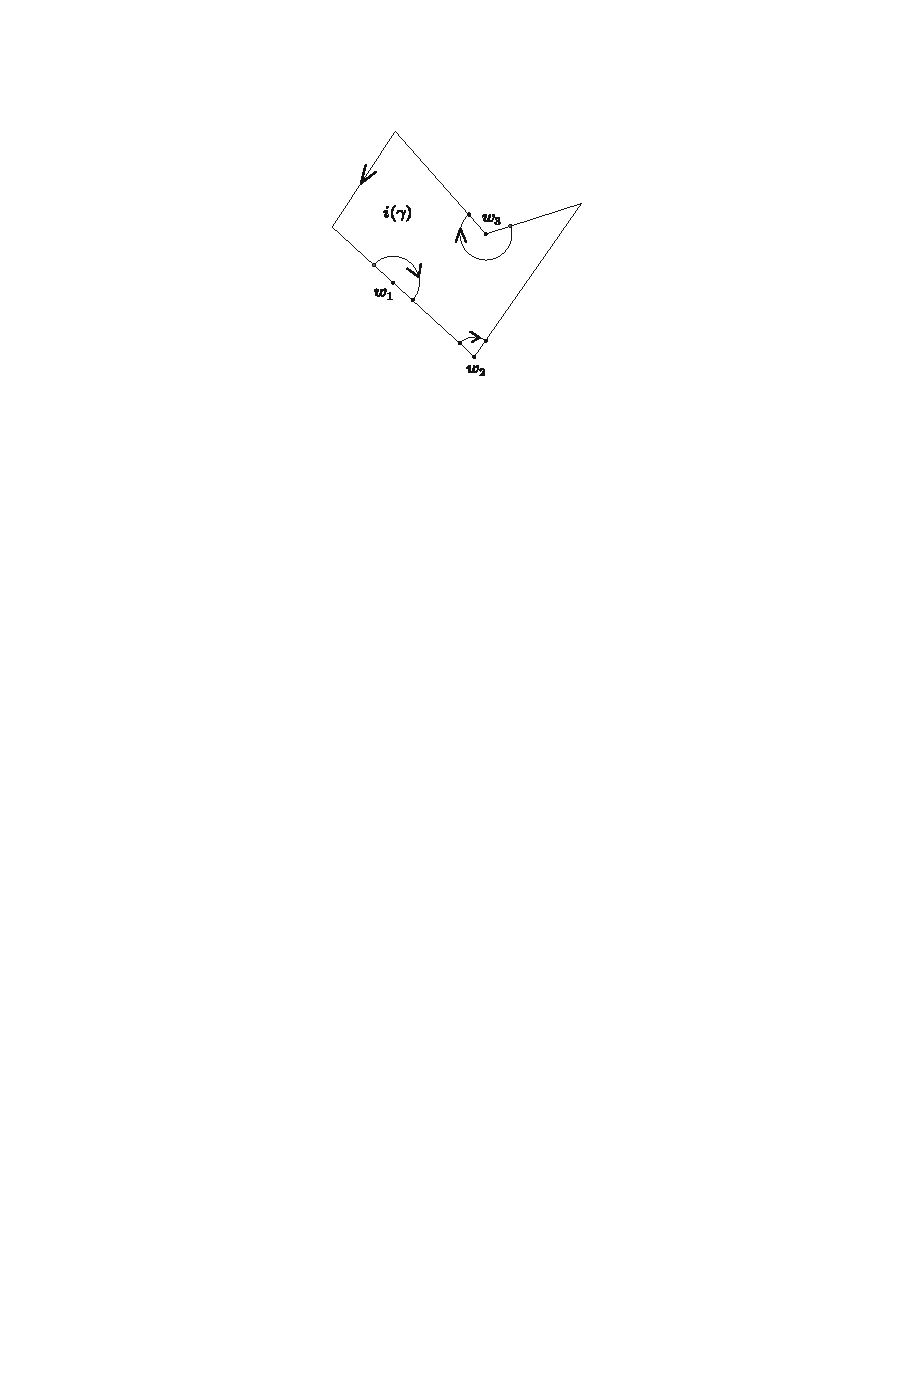
\includegraphics{pictures/modification}
\caption{A modification of a Jordan path.}
\end{figure}

We consider an oriented piecewise differentiable path $\gamma$ in $\C$, and a differential form $\omega=f(z)\dif z$ that is holomorphic in a neighborhood $D$ of $\gamma$ except for isolated singularities on the range of $\gamma$ that are simple poles. Because $\int_{\gamma}\omega$ is not defined, we want to introduce two paths $\gamma$ and $\gamma_{d,\delta}$, the second is disconnected, for which $\int_{\gamma_{\delta}}\omega$ and $\int_{\gamma_{d,\delta}}\omega$ are defined and finite. Let $w_1,\dots,w_m$ be the set of singularities of $\omega$ on $\gamma$. Let $\eps>0$ be the minimum of the finite set consisting of one half the distances between the various $w_k$ and the radii of the largest discs about these points contained in $D$. Let $0<\delta<\eps$. For each $k$, let $C_k$ be the positively oriented circle of radius $\delta$ and center $w_k$. This circle intersects $\gamma$ in a finite set of points. Let $a_{\delta,k}$ be the last point before $w_k$ in this intersection and $b_{\delta,k}$ the first point after $w_k$. These two points define two arcs on $C_k$. Choose one of these arcs; call it $\widetilde{\alpha_{\delta,k}}$, the arc \textbf{subtended at $\bm{w_k}$}, and give it the orientation consistent with that of $\gamma$. Let $-2\pi<\alpha_{\delta,k}<2\pi$ be the angle of this arc measured from $a_{\delta,k}$. The \textbf{$\bm{\delta}$-modification} $\gamma_{\delta}$ of the curve $\gamma$ is obtained by replacing for each $k$ the segment of $\gamma$ between $a_{\delta,k}$ and $b_{\delta,k}$ by the arc $\widetilde{\alpha}_{\delta,k}$. The \textbf{disconnected $\bm{\delta}$-modification} $\gamma_{d,\delta}$ of the curve $\gamma$ is obtained by removing for each $k$ the segment of $\gamma$ between $a_{\delta,k}$ and $b_{\delta,k}$. We define the \textbf{principal value}
\[\text{p.v.}\int_{\gamma}\omega=\lim_{\delta\to 0^+}\int_{\gamma_{d,\delta}}\omega,\]
provided the limit exists.\par
Each of the sets $\{a_{\delta,k}\}$, $\{b_{\delta,k}\}$ and $\{\alpha_{\delta,k}\}$ is bounded. Hence we can construct a sequence $\{\delta_n\}$ that converges to zero with the property that all three sequences have limits denoted by $a_k$, $b_k$, and $\alpha_k$, respectively. Once these limits are known to exist, it is easy to see that the three nets $\{a_{\delta,k}\}$, $\{b_{\delta,k}\}$ and $\{\alpha_{\delta,k}\}$ also converge to the appropriate limits.
\begin{lemma}
Under the hypothesis above, there exists a constant $M>0$ independent of $\delta$ such that
\[\int_{\gamma_{\delta}}\omega-\int_{\gamma_{d,\delta}}\omega=-i\sum_{k=1}^{m}\alpha_{\delta,k}\Res(f,w_k)+\delta\eps(\delta)\]
where $|\eps(\delta)|<M$. Hence
\begin{align}\label{Cauchy integral with sigularity on path}
\lim_{\delta\to 0^+}\Big(\int_{\gamma_{\delta}}\omega-\int_{\gamma_{d,\delta}}\omega\Big)=-i\sum_{k=1}^{n}\alpha_{k}\Res(f,w_k).
\end{align}
\end{lemma}
\begin{proof}
Only the first identity needs verification. Fix $k$. By a translation and rotation, we may assume that $w_k=0$ and $a_k<0$. Write
\[f(z)=\frac{\rho}{z}+g(z)\]
for $|z|<\delta$ with $M_0$ a bound for $|g|$ in $B_{\delta}(0)$. Hence
\[\int_{\widetilde{\alpha}_{\delta,k}}\omega=\int_{\pi}^{\pi-\alpha_{\delta,k}}\Big(\frac{\rho}{\delta e^{i\theta}}+g(\delta e^{i\theta})\Big)\dif(\delta e^{i\theta})=i\rho\int_{\pi}^{\pi-\alpha_{\delta,k}}\dif\theta+i\theta\int_{\pi}^{\pi-\alpha_{\delta,k}}e^{i\theta}g^{\delta e^{i\theta}}\dif\theta.\]
The first of the integrals in the last line is easily evaluated to yield $-\alpha_{\delta,k}$; the absolute value of the second is bounded by $2\pi M_0$. From this the lemma follows.
\end{proof}
\begin{theorem}[\textbf{Residue Theorem with Singularities}]\label{residue theorem with singularities}
Let $\gamma$ be a closed positively oriented Jordan curve in a domain $D$ with $\Int\gamma\sub D$. Let $f$ be a holomorphic function in the domain $D$ except for isolated singularities at $z_1,\dots,z_n$ in $\Int(\gamma)$ and simple poles $w_1,\dots,w_m$ on $\gamma$. Then
\[\mathrm{p.v.}\int_{\gamma}f(z)\dif z=2\pi i\sum_{i=1}^{n}\Res(f,z_i)+i\sum_{k=1}^{m}\alpha_k\Res(f,w_k).\]
\end{theorem}
\begin{proof}
As in previous arguments, $\delta$ is a small positive number, but in this case at most the minimum of the distances from any of the $w_k$ to the $z_i$. By introducing new line segments and thus integrating over a finite number of paths, rather than just a single path, it suffices to assume that $m=1$ and $n=0$. Thus we may take $\gamma$ to be a path in the closure of $\Int\gamma$ from $a_{\delta,1}$ to $w_1$ (where $f(z)\dif z$ has a simple pole) followed by a second one from $w_1$ to $b_{\delta,1}$ and a third from $b_{\delta,1}$ back to $a_{\delta,1}$. As before by translating and rotating the picture we may assume that $w_1=0$ and $a_{\delta,1}<0$. Note that
\[\int_{\gamma_{\delta}}f(z)\dif z=0.\]
From the lemma above,
\[\mathrm{p.v.}\int_{\gamma}f(z)\dif z=i\alpha_1\Res(f,w_1),\]
and this suffices to establish the theorem.
\end{proof}
\section{Sequences and series of holomorphic functions}
\subsection{Consequences of uniform convergence on compact sets}
We begin by recalling some notation and introducing some new symbols. Let $D$ be a domain in $\C$; we denote by $C(D)$ the vector space of continuous complex-valued functions of $D$, and recall that $\mathcal{H}(D)$ is the vector space of holomorphic functions on $D$. We say that a compact disc $\widebar{B_r(z)}$ has rational center if $z=x+iy$ with $x$ and $y$ in $\Q$.
\begin{proposition}
A necessary and sufficient condition for a sequence of functions $\{f_n\}\sub C(D)$ to converge uniformly on all compact subsets of $D$ is for the sequence to converge uniformly on all compact discs with rational centers and rational radii contained in $D$.
\end{proposition}
\begin{proof}
Every compact set contained in $D$ can be covered by finitely many such discs.
\end{proof}
We proceed to describe some consequences of uniform convergence on all compact subsets of $D$, also called locally uniform convergence, for $\mathcal{H}(D)$. The first of these is that $\mathcal{H}(D)$ is closed under locally uniform convergence.
\begin{proposition}\label{holomorphic locally uniform convergence is holomorphic}
If $\{f_n\}\sub\mathcal{H}(D)$ and $\{f_n\}$ converges uniformly on all compact subsets of $D$, then the limit function $f$ is holomorphic on $D$.
\end{proposition}
\begin{proof}
We already know that $f\in C(D)$. Let $\gamma$ be any closed curve null-homotopic in $D$. Then, by Cauchy's theorem,
\[\int_{\gamma}f_n(z)\dif z=0.\]
By uniform convergence it follows that
\[\int_{\gamma}f(z)\dif z=\lim_{n\to+\infty}\int_{\gamma}f_n(z)\dif z=0,\]
and then, by Morera's theorem, $f$ is holomorphic on $D$.
\end{proof}
\begin{corollary}
If $\{f_n\}\sub\mathcal{H}(D)$ and $f=\sum_nf_n$ converges uniformly on all compact subsets of $D$, then the function $f$ is holomorphic on $D$.
\end{corollary}
Theorem~\ref{holomorphic locally uniform convergence is holomorphic} has no analog in real variables: it is easy to see (at least pictorially) that the absolute value function on $\R$, which has no derivative at $0$, can be uniformly approximated by differentiable functions. A more extreme example was constructed by Weierstrass, that of a continuous function defined on $[0,1]$ which is nowhere differentiable and uniformly approximated by
polynomials.\par
We will shortly see that uniform convergence of a sequence of holomorphic functions on all compact subsets of their common domain of definition implies uniform convergence of the derivatives on the same sets. This is another feature of holomorphic functions not shared by real differentiable functions: it is easy to construct a sequence of differentiable functions converging uniformly on a closed interval with the property that the sequence of derivatives does not converge uniformly there.
\begin{theorem}\label{holomorphic locally uniform convergence derivative}
If $\{f_n\}\sub\mathcal{H}(D)$ and $\{f_n\}$ converges to $f$ uniformly on all compact subsets of $D$, then $\{f_n'\}$ converges to $f'$ uniformly on all compact subsets of $D$.
\end{theorem}
\begin{proof}
Since $f\in\mathcal{H}(D)$, it is enough to check uniform convergence of the derivatives on all compact subdiscs $K\sub D$, with $\partial K=\gamma$ positively oriented. For $z\in\Int\gamma$ we have
\[f'(z)=\frac{1}{2\pi i}\int_{\gamma}\frac{f(\zeta)\dif\zeta}{(\zeta-z)^2}=\lim_{n\to+\infty}\frac{1}{2\pi i}\int_{\gamma}\frac{f_n(\zeta)\dif\zeta}{(\zeta-z)^2}=\lim_{n\to+\infty}f_n'(z)\]
this convergence is uniform in any smaller compact subdisc, such as
\[\widetilde{K}=\{z\in\Int\gamma:|z-w|\geq\delta>0\text{ for all }w\in\im\gamma\}.\]
with $\delta$ sufficiently small.
\end{proof}
\begin{theorem}\label{holomorphic sequence no root}
Let $\{f_n\}$ be a sequence of holomorphic functions on $D$ such that $f_n$ converges to $f$ uniformly on all compact subsets of $D$. If $f_n$ has no root in $D$ for all $n>0$, then either
\begin{itemize}
\item $f$ is identically zero, or
\item $f$ has no root in $D$.
\end{itemize}
\end{theorem}
\begin{proof}
Assume that $z_0\in D$ is a root of $f$ and that $f$ is not identically zero. Then there exists a circle $\gamma$ with center $z_0$ such that $\Int\gamma\sub D$ and $f(z)\neq 0$ for all $z\in\widebar{\Int(\gamma)}\setminus\{z_0\}$. By the argument principle, the number $N$ of zeros of $f$ in $\Int(\gamma)$ is given by
\[N=\frac{1}{2\pi i}\int_{\gamma}\frac{f'(z)}{f(z)}\dif z=1.\]
But
\[\frac{1}{2\pi i}\int_{\gamma}\frac{f'(z)}{f(z)}\dif z=\lim_{n\to+\infty}\frac{1}{2\pi i}\int_{\gamma}\frac{f_n'(z)}{f_n(z)}\dif z=0.\]
This is a contradiction.
\end{proof}
An equivalent formulation for this theorem is the following, sometimes referred to as Hurwitz's theorem.
\begin{theorem}[\textbf{Hurwitz}]
Let $\{f_n\}$ be a sequence of holomorphic functions on $D$ such that $f_n$ converges to $f$ uniformly on all compact subsets of $D$, and assume $f$ is not identically zero on $D$. For every disc $U$ such that $\widebar{U}\sub D$ with the property that $f\neq 0$ on $\partial U$, there exists $N>0$ such that $f$ and $f_n$ have the same number of zeros in $U$ for all $n\geq N$.
\end{theorem}
\begin{proof}
This is proved by the equality
\[\frac{1}{2\pi i}\int_{\partial U}\frac{f'(z)}{f(z)}\dif z=\lim_{n\to+\infty}\frac{1}{2\pi i}\int_{\partial U}\frac{f_n'(z)}{f_n(z)}\dif z.\]
Note that both sides are integers.
\end{proof}
The Hurwitz's theorem is particularly useful for the injectivity of a limit function. More precisely, we introduce the following definition.
\begin{definition}
Let $f\in \mathcal{H}(D)$. We call $f$ \textbf{simple}, \textbf{univalent}, or \textbf{schlicht} if it is one-to-one (injective) on $D$; thus a homeomorphism onto $f(D)$.
\end{definition}
\begin{theorem}[\textbf{Hurwitz}]\label{holomorphic univalent sequence}
Assume $D$ is a domain in $\C$. If $\{f_n\}$ is a sequence in $\mathcal{H}(D)$ with $f_n\to f$ uniformly on all compact subsets of $D$ and $f_n$ is univalent for each $n$, then either $f$ is constant or univalent.
\end{theorem}
\begin{proof}
Assume that $f$ is neither constant nor univalent; thus, in particular, there exist $z_1$ and $z_2$ in $D$ with $z_1\neq z_2$ and $f(z_1)=f(z_2)$. For each $n>0$, set $g_n=f_n(z)-f_n(z_2)$ on the domain $D'=D\setminus\{z_2\}$. Then $g_n\in\mathcal{H}(D')$, $g_n$ never vanishes in $D'$ and $g_n\to f(z)-f(z_2)$ uniformly on all compact subsets of $D'$. But $g$ is not identically zero and vanishes at $z_1$; we have thus obtained a contradiction to Theorem~\ref{holomorphic sequence no root}.
\end{proof}
\subsection{A metric on the space of continuous functions}
We introduce, for use in the proof of the compactness theorem and in the proof of the Riemann mapping theorem, a metric on $C(D)$ for any domain $D$ in $\C$. The metric $d$ on $C(D)$ will have the property that convergence in this metric is equivalent to uniform convergence on all compact subsets of $D$.\par
For $K$ compact in $D$ and $f\in C(D)$, set
\[\|f\|_K=\max\{|f(z)|:z\in K\}.\]
Consider the set of compact (closed) discs contained in $D$ with rational radii and rational centers. There are countably many such discs and they cover $D$. Call this collection of discs $\{D_i\}$. For each $n>0$, let
\[K_n=\bigcup_{i=1}^{n}D_i\]
then $\{K_n\}$ is an exhaustion of $D$ by compact subsets. A crucial consequence that we will use often is that given an exhaustion $\{K_n\}$ of $D$, each compact subset $K$ of $D$ is contained in $K_n$ for some $n$.\par
With this preparation, we define a norm on $C(D)$ by letting
\[\|f\|=\sum_{n=1}^{\infty}2^{-n}\min\{1,\|f\|_{K_n}\}\]
for $f\in C(D)$.
\begin{lemma}\label{property of norm on C(D)}
For all $f$ and $g\in C(D)$:
\begin{itemize}
\item[(a)] $\|f\|\geq 0$, and $\|f\|=0$ if and only if $f\equiv 0$.
\item[(b)] $\|f+g\|\leq\|f\|+\|g\|$.
\item[(c)] For each $n$, $2^{-n}\|f\|_{K_n}\leq \|f\|$.
\item[(d)] For each $n$, $\|f\|\leq \|f\|_{K_n}+2^{-n}$.
\end{itemize}
\end{lemma}
\begin{proof}
We only prove (d):
\begin{align*}
\|f\|&=\sum_{i=1}^{n}2^{-i}\min\{1,\|f\|_{K_i}\}+\sum_{i=n+1}^{\infty}2^{-i}\min\{1,\|f\|_{K_i}\}\\
&\leq\sum_{i=1}^{n}2^{-i}\|f\|_{K_n}+\sum_{i=n+1}^{\infty}2^{-i}\\
&\leq\|f\|_{K_n}+2^{-n}.
\end{align*}
This completes the proof.
\end{proof}
With this norm, the metric $d$ is given by
\[d(f,g)=\|f-g\|.\]
We now establish some properties of the metric $d$.
\begin{lemma}
For all $f$, $g$, and $h$ in $C(D)$, the following hold:
\begin{itemize}
\item[(a)] $d(f,g)\geq 0$, and $d(f,g)=0$ if and only if $f=g$.
\item[(b)] $d(f,g)=d(g,f)$.
\item[(c)] $d(f,g)\leq d(f,h)+d(h,g)$.
\item[(d)] $d(f+h,g+h)=d(f,g)$, that is, $d$ is translation invariant.
\item[(e)] $d(f,g)\leq 1$; that is, $d$ is a bounded metric.
\end{itemize}
\end{lemma}
\begin{theorem}\label{comverge in C(D) metric iff locally uniform on compact}
Convergence in the $d$-metric in $C(D)$ is equivalent to uniform convergence on all compact subsets of $D$.
\end{theorem}
\begin{proof}
Let $\{f_n\}\sub C(D)$ and assume that $\{f_n\}$ is $d$-convergent. Since for every compact set $K\sub D$ there is an $i>0$ such that $K\sub K_i$, it suffices to show uniform convergence on $K_i$ for each $i$.\par
Given $0<\eps<1$, we can choose $N>0$ large so that
\[d(f_m,f_n)\leq d(f_m,f)+d(f_n,f)<2^{-i}\eps.\]
for $m,n\geq N$. This then implies $\|f_m-f_n\|_{K_i}<2^{-i}\eps$, so the sequence $\{f_n\}$ converges uniformly on $K_i$.\par
We have actually shown more than claimed: if $\{f_n\}$ is a $d$-Cauchy sequence in $C(D)$, then there exists an $f\in C(D)$ such that $f_n\to f$ uniformly on all compact subsets of $D$.\par
Conversely, assume that $f_n\to f$ uniformly on $K_n$ for all $n$. Thus for all $n>0$,
\[\lim_{i\to+\infty}\|f-f_i\|_{K_n}=0.\]
Given $\eps>0$, first choose $i$ such that $2^{-i}<\eps/2$ and next choose $N$ such that $\|f-f_n\|_{K_i}$ for all $n\geq N$. Then
\[\|f-f_n\|\leq\|f-f_n\|_{K_i}+2^{-i}<\eps/2+\eps/2=\eps.\]
Therefore $f_n\to f$ in $d$-metric.
\end{proof}
\begin{corollary}
The topology of the metric space $(C(D),d)$ is independent of the choice of exhaustion $\{K_n\}$ of $D$.
\end{corollary}
\begin{corollary}
$d$ is a complete metric on $C(D)$.
\end{corollary}
Because of Theorem~\ref{comverge in C(D) metric iff locally uniform on compact}, we can reformulate the results of the previous part in terms of the metric $d$. In particular, Theorems~\ref{holomorphic locally uniform convergence is holomorphic} and \ref{holomorphic locally uniform convergence derivative} can now be phrased as in the following corollary. We already remarked that $\mathcal{H}(D)\sub C(D)$, so $d$ restricts to a metric to $\mathcal{H}(D)$, also denoted by $d$.
\begin{corollary}
$\mathcal{H}(D)$ is a closed subspace of $C(D)$, thus a complete metric space. Furthermore, $f\mapsto f'$ is a continuous linear operator from $\mathcal{H}(D)$ to itself.
\end{corollary}
There is an alternate description of the topology induced by $d$, that is, the topology of the metric space $(C(D),d)$. Given $f\in C(D)$, $K\sub D$ compact and $\eps>0$, we define
\[V_f(K,\eps)=\{g\in C(D):\|g-f\|_{K}<\eps\}.\]
We will now show that the collection
\[\{V_f(K,\eps):K\sub D\text{ compact and }\eps>0\}\]
is a basis for the neighborhood system at $f$.
\begin{theorem}\label{basis for C(D)}
For any $f\in C(D)$, a basis for the neighborhood system at $f$ (with respect to the topology induced by $d$ on $C(D)$) is given by the sets $V_f(K,\eps)$.
\end{theorem}
\begin{proof}
It is enough to show that
\begin{itemize}
\item[(a)] Given $V_{f}(K,\eps)$, there exists an $B_{\delta}(f)\sub V_f(K,\eps)$.
\item[(b)] Given $B_\delta(f)$, there exists a $V_f(K,\eps)\sub B_\delta(f)$. 
\end{itemize}
To show (a), we assume without loss of generality that $0<\eps<1$. Choose $i$ such that $K\sub K_i$ and set $\delta=\eps/2^i$. If $g\in N_f(\delta)$, then $\|f-g\|<\eps/2^i$. Thus
\[2^{-i}\min\{1,\|g-f\|_{K_i}\}<\eps/2^i\]
and then $\|g-f\|_{K_i}<\eps$. But
\[\|g-f\|_K\leq\|g-f\|_{K_i};\]
that is, $g\in V_f(K,\eps)$.\par
To show (b), choose $i$ such that $2^{-i}<\delta/2$. For $g\in V_f(K_i,\delta/2)$, we have $\|g-f\|_{K_i}<\delta/2$. Hence
\[d(g,f)<\|g-f\|_{K_i}+2^{-i}<\delta.\]
that is, $g\in B_{\delta}(f)$.
\end{proof}
We can apply these concepts to convergence of series of meromorphic functions.
\begin{definition}
Let ffng be a sequence in $\mathcal{M}(D)$, the meromorphic functions on $D$. We say that $\sum_nf_n$ \textbf{converges uniformly (absolutely)} on a subset $A$ of $D$ if there exists an integer $N$ such that $f_n$ is holomorphic on $A$ for all $n>N$ and $\sum_{n=N+1}^{\infty}f_n$ converges uniformly (absolutely) on $A$.
\end{definition}
\begin{proposition}
Let $\{f_n\}\sub\mathcal{M}(D)$. If $\sum_nf_n$ converges uniformly on all compact subsets of $D$, then the series $f=\sum_nf_n$ is a meromorphic function on $D$, and $\sum_nf_n'$ converges uniformly on all compact subsets to $f'$.
\end{proposition}
\subsection{The cotangent function}
As an application of the ideas developed in the last two parts, we establish a series expansion formula for the cotangent function.
\begin{theorem}\label{cotangent function expansion}
For all $z$ in $\C\setminus\Z$ the following equalities hold:
\begin{align}\label{cotangent function expansion-1}
\pi\cot\pi z=\frac{1}{z}+\sum_{n\in\Z,n\neq 0}\Big(\frac{1}{z-n}-\frac{1}{n}\Big)=\frac{1}{z}+\sum_{n=1}^{\infty}\frac{2z}{z^2-n^2}.
\end{align}
\end{theorem}
First of all, we claim that
\[\sum_{n\in\Z,n\neq 0}\Big(\frac{1}{z-n}-\frac{1}{n}\Big)=\sum_{n\neq 0}^{\infty}\frac{z}{n(z-n)}\]
converges absolutely and uniformly on all compact subsets of $\C$. To verify this claim, assume that $|z|<R$ with $R>0$. Then
\[\sum_{|n|>2R}\frac{|z|}{|n||z-n|}\leq\sum_{n\geq 2R}\frac{|R|}{|n|(|n|-R)}\leq\sum_{|n|\geq 2R}\frac{2R}{|n|^2}<+\infty.\]
We can now verify the expansion $(\ref{cotangent function expansion-1})$ for $\pi\cot\pi z$.
\begin{proof}[Proof of Theorem~\ref{cotangent function expansion}]
For $N>0$, let $C_N$ be the positively oriented boundary of the square with vertices $(N+1/2)(\pm 1+\pm i)$. Then
\[\frac{1}{2\pi i}\int_{C_N}\frac{\cot\pi\zeta}{\zeta-z}\dif\zeta=\sum_{z\in\Int C_N}\Res\Big(\frac{\cot\pi\zeta}{\zeta-z},z\Big).\]
Here $z\in\C$ is fixed: we take $z\in\Int C_N$ and $z\notin\Z$. The poles of the function $H(\zeta)=\cos\pi\zeta/(\zeta-z)$ occur at $\zeta=z$ and at $\zeta=n\in\Z$, and they are all simple. Furthermore, we see that
\[\Res\Big(\frac{\cot\pi\zeta}{\zeta-z},z\Big)=\cot\pi z,\quad \Res\Big(\frac{\cot\pi\zeta}{\zeta-z},n\Big)=\lim_{\zeta\to n}(\zeta-n)\frac{\cos\pi\zeta}{\sin\pi\zeta}\frac{1}{\zeta-z}=\frac{1}{\pi(n-z)}.\]
Thus we have
\[\frac{1}{2\pi i}\int_{C_N}\frac{\cot\pi\zeta}{\zeta-z}\dif\zeta=\cos\pi z+\frac{1}{\pi}\sum_{n=-N}^{N}\frac{1}{\pi(n-z)}=\cos\pi z+\frac{1}{\pi}\sum_{|n|\leq N,n\neq 0}\Big(\frac{1}{n-z}-\frac{1}{n}\Big)+\frac{1}{\pi z}.\]
Hence it sufficies to prove
\begin{align}\label{cotangent function expansion-2}
\lim_{N\to+\infty}\frac{1}{2\pi i}\int_{C_N}\frac{\cot\pi\zeta}{\zeta-z}\dif\zeta=0.
\end{align}
We proceed in stages. We first note that
\begin{align*}
\frac{1}{2\pi i}\int_{C_N}\frac{\cot\pi\zeta}{\zeta}\dif\zeta&=\sum_{z\in\Int C_N}\Res\Big(\frac{\cot\pi\zeta}{\zeta},z\Big)=\Res\Big(\frac{\cot\pi\zeta}{\zeta},0\Big)+\sum_{|n|\leq N,n\neq 0}\Big(\frac{\cot\pi\zeta}{\zeta},n\Big)\\
&=\Res\Big(\frac{\cot\pi\zeta}{\zeta},0\Big)+\sum_{|n|\leq N,n\neq 0}\frac{1}{\pi n}=0.
\end{align*}
The last sum is clearly zero, and the residue of $\cos\pi\zeta/\zeta$ at zero is $0$ because it is an even function. With this observation, we have
\begin{align}\label{cotangent function expansion-3}
\int_{C_N}\frac{\cot\pi\zeta}{\zeta-z}\dif\zeta=\int_{C_N}\cot\pi\zeta\Big(\frac{1}{\zeta-z}-\frac{1}{\zeta}\Big)\dif\zeta=\int_{C_N}\frac{z\cot\pi\zeta}{\zeta(\zeta-z)}\dif\zeta.
\end{align}
We calim that there exists an $M>0$ (independent of $N$) such that $|\cos\pi\zeta|\leq M$ for all $z\in C_N$. In fact, write $\zeta=u+iv$, then
\begin{align*}
|\cot\pi\zeta|^2=\frac{\cos^2\pi u+\sinh^2\pi v}{\sin^2\pi u+\sinh^2\pi v}.
\end{align*}
On the vertical sides of $C_N$ we have $u=\pm N\pm 1/2$, so
\begin{align}\label{cot function bounded on vertical}
|\cot\pi\zeta|^2=\frac{\sinh^2\pi v}{1+\sinh^2\pi v}\leq 1.
\end{align}
On the horizontal sides of $C_N$, $v=\pm N\pm 1/2$ and hence
\begin{align}\label{cot function bounded on horizontal}
|\cot\pi\zeta|^2=\frac{\cos^2\pi u+\sinh^2\pi(\pm N\pm 1/2)}{\sin^2\pi u+\sinh^2\pi(\pm N\pm 1/2)}\leq\frac{1+\sinh^2\pi(\pm N\pm 1/2)}{\sinh^2\pi(\pm N\pm 1/2)}\to 1.
\end{align}
Thus there exists an $M>0$ such that $|\cot\pi\zeta|\leq M$ for $\zeta$ on the horizontal sides of $C_N$, and the claim is proved.\par
If we denote by $L(C_N)$ the length of $C_N$, then by $(\ref{cotangent function expansion-3})$,
\begin{align*}
\Big|\int_{C_N}\frac{\cot\pi\zeta}{\zeta-z}\dif\zeta\Big|&=\Big|\int_{C_N}\frac{z\cot\pi\zeta}{\zeta(\zeta-z)}\dif\zeta\Big|\leq\int_{C_N}\frac{M|z|}{|\zeta||\zeta-z|}\,|\mathrm{d}\zeta|\\
&\leq\frac{M|z|}{(N+1/2)(N+1/2-|z|)}L(C_N)=\frac{8M|z|}{(N+1/2-|z|)}\to 0.
\end{align*}
Thus $(\ref{cotangent function expansion-2})$ is proved.
\end{proof}
Differentiating the series $(\ref{cotangent function expansion})$ term by term, we obtain the following expansion.
\begin{corollary}
For all $z\in\C\setminus\Z$,
\[\frac{\pi^2}{\sin^2\pi z}=\sum_{n=-\infty}^{\infty}\frac{1}{(z-n)^2}.\]
\end{corollary}
As an application of the cotangent expansion. We give the special values of the Riemann zeta function at even numbers. First, recall that the \textbf{Bernoulli numbers} $B_n$ are given by the Taylor series
\[\frac{z}{e^z-1}=B_0+B_1z+\sum_{n=1}^{\infty}\frac{B_{2n}}{(2n)!}z^{2n}\]
and we already know that $B_0=1$ and $B_1=-1/2$.
\begin{theorem}
The values of the Riemann zeta function at the even natural numbers are given by the Euler formula:
\[\zeta(2k):=\sum_{n=1}^{\infty}\frac{1}{n^{2k}}=\frac{(-1)^{k+1}(2\pi)^{2k}}{2(2k)!}B_{2k}.\]
\end{theorem}
\begin{proof}
By the definition of $\cot z$, we have
\begin{align*}
z\cot z&=iz\frac{e^{iz}+e^{-iz}}{e^{iz}-e^{-iz}}=iz\frac{e^{2iz}+1}{e^{2iz}-1}=\frac{2iz}{e^{2iz}-1}+iz\\
&=iz+1-\frac{2iz}{2}+\sum_{k=1}^{\infty}\frac{B_{2k}}{(2k)!}(iz)^{2k}=1+\sum_{k=1}^{\infty}(-1)^k\frac{B_{2k}}{(2k)!}(z)^{2k}.
\end{align*}
We replace $z$ by $\pi z$, and obtain
\begin{align}\label{compute zeta(2k)}
\pi z\cot\pi z=1+\sum_{k=1}^{\infty}(-1)^k\frac{(2\pi)^{2k}}{(2k)!}B_{2k}z^{2k}
\end{align}
in a suitable neighborhood of $0$. On the other side, we already now that
\[\pi z\cot\pi z=1+\sum_{n=1}^{\infty}\frac{2z^2}{z^2-n^2}1+2z^2\sum_{n=1}^{\infty}\Big(-\frac{1}{n^2}\sum_{k=0}^{\infty}\Big(\frac{z^2}{n^2}\Big)^k\Big)=\pi z\cot\pi z=1-2\sum_{k=1}^{\infty}\Big(\sum_{n=1}^{\infty}\frac{1}{n^{2k}}\Big)z^{2k}.\]
Comparing with $(\ref{compute zeta(2k)})$ we can isolate the values of $\zeta(2k)$.
\end{proof}
\subsection{Compact sets in $\mathcal{H}(D)$}
We return to the study of $C(D)$ with the $d$-metric.
\begin{definition}
Let $\mathscr{F}\sub C(D)$. We say that $\mathscr{F}$ is \textbf{locally bounded} if $\mathscr{F}$ is uniformly bounded on compact subsets; that is, if for each compact $K\sub D$, there exists an $M(K)>0$ such that $\|f\|_K\leq M(K)$ for all $f\in\mathscr{F}$.
\end{definition}
The importance of locally boundedness is revealed in the following theorem.
\begin{theorem}\label{holomorphic locally bounded is equicontinuous}
Let $A\sub\mathcal{H}(D)$ be locally bounded. Then $A$ is equicontinuous. 
\end{theorem}
\begin{proof}
Let $K$ be a compact subset of $D$ and choose $r>0$ so small that $B_{3r}(z)$ is contained in $D$ for all $z\in K$. Let $z,w\in K$ with $|z-w|<r$, and let $\gamma$ denote the boundary circle of the disc $B_{2r}(w)$. Then, by Cauchy's integral formula, we have
\[f(z)-f(w)=\frac{1}{2\pi i}\int_{\gamma}f(\zeta)\Big[\frac{1}{\zeta-z}-\frac{1}{\zeta-w}\Big]\dif\zeta.\]
Observe that
\[\Big|\frac{1}{\zeta-z}-\frac{1}{\zeta-w}\Big|=\frac{|z-w|}{|\zeta-z||\zeta-w|}\leq\frac{|z-w|}{r^2}.\]
since $\zeta\in\gamma$ and $|z-w|<r$. Therefore
\[|f(z)-f(w)|\leq\frac{1}{2\pi}\frac{2\pi r}{r^2}M|z-w|=\frac{M}{r}|z-w|\]
where $M$ denotes the uniform bound for $A$ in the compact set consisting of all points in $D$ at a distance $\leq 2r$ from $K$. Therefore $|f(z)-f(w)|<C|z-w|$, and this estimate is true for all $z,w\in K$ with $|z-w|<r$ and $f\in\mathscr{F}$; thus this family is equicontinuous, as was to be shown.
\end{proof}
\begin{theorem}[\textbf{Compactness Theorem}]\label{holomorphic compact theorem}
Let $D$ be a domain in $\C$. Then every a subset $\mathscr{F}$ of $\mathcal{H}(D)$ is compact if and only if it is closed and locally bounded.
\end{theorem}
\begin{proof}
If $\mathscr{F}$ is closed and locally bounded, then it is equicontinuous by Theorem~\ref{holomorphic locally bounded is equicontinuous}, so it follows from Proposition~\ref{Arzela-Ascoli convergent subsequence} that $A$ is compact in $\mathcal{H}(D)$.\par
Conversely, if $\mathscr{F}$ is compact, then it is closed. Moreover, for each compact subset, the function $f\mapsto\|f\|_K$ is continuous on the compact set $\mathscr{F}$. Thus it is a bounded function, and hence $\mathscr{F}$ is locally bounded.
\end{proof}
\begin{corollary}[\textbf{Montel's Theorem}]
Every locally bounded subset in $\mathcal{H}(D)$ is precompact.
\end{corollary}
Note that the converse to Montel's theorem also holds.
\begin{theorem}[\textbf{Vitali's Theorem}]
Let $D$ be a domain in $\C$, and assume that the elements in a sequence $\{f_n\}$ are locally bounded in $\mathcal{H}(D)$. Let $S\sub D$ and assume that $S$ has a limit point in $D$. If $\lim_{n}f_n(z)$ exists for all $z\in S$, then the sequence $\{f_n\}$ converges in $\mathcal{H}(D)$.
\end{theorem}
\begin{proof}
The assumptions imply that the set $\{f_n\}$ is precompact, so $\{f_n\}$ has a limit point $f$ in $\mathcal{H}(D)$. If $f$ and $g$ are both limit points of $\{f_n\}$, then
\[f(z)=\lim_nf_n(z)=g(z)\]
for $z\in S$. Since $S$ has a limit point in $D$, this implies $f=g$. Therefore the set $\{f_n\}$ has a unique limit point $f$ in $\mathcal{H}(D)$, which means $f_N$ converges to $f$ in $\mathcal{H}(D)$.
\end{proof}
\subsection{Runge's Theorem}
We consider the problem of approximating holomorphic functions by rational
functions. We regard a nonconstant polynomial as a rational function whose only pole is at infinity. The ability to uniformly approximate a holomorphic function depends on the region where the function is being approximated, as well as upon the function itself. The strongest statement about uniform approximation of holomorphic functions that we prove is Runge's approximation theorem. A number of proofs appear in the literature; ours is a variant of these.\par
We have already proved a form of Runge's theorem for an open disc $D$: a holomorphic function on $D$ has a power series expansion at the center of the disc; for every positive integer $n$, we obtain a polynomial of degree $n$ by discarding all the higher order terms in the series. These polynomials converge to the function uniformly on any compact subset of the disc.\par
On the other hand, we also know that uniform polynomial approximation does not hold in general. For instance, consider a punctured disc $D=\{0<|z-z_0|<R\}$, with $R>0$ and $z_0$ arbitrary, and the analytic function on defined by $f(z)=1/(z-z_0)$ (we take advantage of the fact that it is a rational function whose only pole is at $z_0$); if $f$ were uniformly approximated by a sequence of polynomials $\{p_n\}$ in the closed annulus $K=\{0<r\leq|z-z_0|\leq\rho<R\}$, then by taking $\gamma(\theta)=(r+\rho)e^{i\theta}/2$ for $0\leq\theta\leq 2\pi$ we would obtain the contradiction that
\[0=\lim_{n\to+\infty}\int_{\gamma}p_n(z)\dif z=\int_{\gamma}f(z)\dif z=2\pi i.\]
However, truncation of the Laurent series expansion for $f$ on $f$ shows that $f$ is indeed uniformly approximated on $K$ by rational functions whose poles lie outside $D$. This fact is generalized to arbitrary open sets $D$.
\begin{theorem}[\textbf{Runge}]\label{Runge theorem}
Let $K$ be a compact subset of $\C$ and let $S$ be a subset of $\widehat{\C}\setminus K$ that intersects nontrivially each connected component of $\widehat{\C}\setminus K$. If $f$ is a holomorphic function on an open set $D$ containing $K$, then it can be uniformly approximated on $K$ by rational functions with simple poles lying on $S$; that is, for every $\eps>0$ there exists a rational function $R$ with possibly simple poles only in $S$ such that $|f(z)-R(z)|<\eps$ for all $z\in K$.
\end{theorem}
We can always choose for $S$ a smallest set consisting of one point from each connected component of $\widehat{\C}\setminus K$. For the important special case where $\widehat{\C}\setminus K$ is connected and $S$ is chosen as $S=\{\infty\}$, Runge's theorem asserts that each function that is analytic in an open neighborhood of $K$ can be uniformly approximated in $K$ by a sequence of polynomials.\par
Before we start the proof, let's establish an extension of Cauchy's integral formula, which will be used later.
\begin{proposition}\label{cauchy integral formula extended form}
Let $K$ be a compact subset of $\C$ and let $D$ be an open set containing $K$. Then there exists a finite collection of oriented line segments $\gamma_1,\dots,\gamma_n$ in $D\setminus K$ such that for every holomorphic function $f$ on $D$,
\begin{align}\label{cauchy integral formula extended form-1}
f(z)=\frac{1}{2\pi i}\sum_{i=1}^{n}\int_{\gamma_i}\frac{f(\zeta)}{\zeta-z}\dif\zeta
\end{align}
for all $z\in K$.
\end{proposition}
\begin{proof}
After enlarging $K$ if necessary, we may assume that $K=\overline{\Int K}$. For example, we enlarge $K$ if it consists of a single point. For any positive real number $\delta$ we consider a rectangular grid of horizontal and vertical lines in the plane $\C$ so that consecutive parallel lines are at distance $\delta$ apart. We let $R_1,\dots,R_m$ be the rectangles in the grid that have nonempty intersection with $K$. Since $K$ is compact, there are only a finite number of such rectangles. We can (and from now on do) choose $\delta$ such that $R_i\sub D$ for all $i$; if $D=\C$ any $\delta>0$ suffices, and otherwise it is enough to consider any $0<\delta<d(K,D^c)/2$, since $z\in R_i$ implies that $d(z,K)<\sqrt{2}\delta$. As usual, the boundary of $R_i$ is denoted by $\partial R_i$ and is oriented in the counterclockwise direction. The integrals of a continuous form along the common boundaries of any pair of contiguous $R_i$ and $R_j$ cancel out. This last observation implies that we can choose a set $\mathcal{S}$ of curves whose ranges are a subset of the sides in $\bigcup_{i=1}^{m}\partial R_i$, and such that the set $\mathcal{S}=\{\gamma_i:1\leq i\leq n\}$ satisfies
\begin{itemize}
\item[(a)] If $\gamma_i$ is in $\mathcal{S}$, it lies on a side of only one $R_i$.
\item[(b)] If $\gamma_i$ is in $\mathcal{S}$, then it is disjoint from $K$.
\item[(c)] For any continuous function $g$ on $\bigcup_{i=1}^{m}\partial R_i$, we have
\begin{align}\label{cauchy integral formula extended form-2}
\sum_{i=1}^{m}\int_{\partial R_i}g(z)\dif z=\sum_{i=1}^{n}\int_{\gamma_i}g(z)\dif z.
\end{align}
\end{itemize}
Each $\gamma_i$ is an oriented line segment in $D\setminus K$. It remains to prove that equation $(\ref{cauchy integral formula extended form-1})$ holds with these $\gamma_i$. If $z\in K$ and $z$ is not on the boundary of any of the rectangles, then the function
\[\zeta\mapsto g(\zeta)=\frac{1}{2\pi i}\frac{f(\zeta)}{\zeta-z},\quad \zeta\in\bigcup_{i=1}^{m}\partial R_i.\]
is continuous. Thus, we have, by $(\ref{cauchy integral formula extended form-2})$,
\[\frac{1}{2\pi i}\sum_{i=1}^{m}\int_{\partial R_i}\frac{f(\zeta)}{\zeta-z}\dif\zeta=\frac{1}{2\pi i}\sum_{i=1}^{n}\int_{\gamma_i}\frac{f(\zeta)}{\zeta-z}\dif\zeta.\]
Assume that $z$ belongs to the interior of exactly one of the $R_i$, call it $R_t$. If $i\neq t$, then $z\notin R_i$ and so
\[\frac{1}{2\pi i}\int_{\partial R_i}\frac{f(\zeta)}{\zeta-z}\dif\zeta=0,\]
also, since $z\in R_t$, by Cauchy's integral formula, we have
\[\frac{1}{2\pi i}\int_{\partial R_t}\frac{f(\zeta)}{\zeta-z}\dif\zeta=f(z).\]
Thus $(\ref{cauchy integral formula extended form-1})$ holds for all $z\in R_t$. Since range $\gamma_i$ does not intersect $K$, both sides of this equation are continuous functions of $z$ on $K$, and they agree on the set of points $z$ in $K$ that are not on the boundary of any rectangle $R_i$, a dense subset of $K$. Thus they agree for all $z\in K$.
\end{proof}
Let $K$ and $S$ be the sets described in the hypothesis of Runge's theorem, and define $B(K,S)$ be the closure in the space $C(K)$ of rational functions with poles only in $S$. Runge's theorem asserts that every holomorphic function on a neighborhood of $K$ belongs to $B(S,K)$. The main tool in proving Runge's Theorem is Proposition~\ref{pair annihilator prop} and Riesz's representation theorem. First, we need the following lemma.
\begin{lemma}\label{Runge lemma}
Let $\lambda$ be the Lebesgue measure on $\C$. If $\mu\in M(K)$, then the function
\[\hat{\mu}(z)=\int_K\frac{d\mu(\zeta)}{\zeta-z}\]
is in $L^1_{loc}(\lambda)$, analytic on $\widehat{\C}\setminus K$, and $\hat{\mu}(\infty)=0$.
\end{lemma}
\begin{proof}
Let $R>0$, we prove that $\hat{\mu}(z)$ is integrable on $B_r(0)$. To see this, note that
\begin{align*}
\int_{B_r(0)}\Big|\int_K\frac{d\mu(\zeta)}{\zeta-z}\Big|\,d\lambda(z)\leq\int_{B_r(0)}\int_K\frac{d|\mu|(\zeta)}{|\zeta-z|}\,d\lambda(z)=\int_K\int_{B_r(0)}\frac{d\lambda(z)}{|\zeta-z|}\,d|\mu|(\zeta).
\end{align*}
Choose $\rho>0$ such that $B_R(0)\sub B_\rho(z)$, for each $z\in K$. We then have
\[\int_{B_r(0)}\Big|\int_K\frac{d\mu(\zeta)}{\zeta-z}\Big|\,d\lambda(z)\leq\int_{K}\int_0^{2\pi}\int_0^\rho drd\theta d|\mu|(\zeta)=2\pi\rho\|\mu\|.\]
Thus $\hat{\mu}\in L^1_{loc}(\lambda)$, and $\hat{\mu}$ is well defined. To show that $\hat{\mu}$ is analytic on $\widehat{\C}\setminus K$, let $z,z_0\in K$ and note that
\[\frac{\hat{\mu}(z)-\hat{\mu}(z_0)}{z-z_0}=\int_K\frac{d\mu(\zeta)}{(\zeta-z)(\zeta-z_0)}.\]
Since $[(\zeta-z)(\zeta-z_0)]^{-1}\to(\zeta-z_0)^{-2}$ uniformly on $K$, as $z\to z_0$, $\hat{\mu}$ has a derivative and 
\[\frac{d}{dz}\hat{\mu}(z)=\int_K\frac{d\mu(\zeta)}{(\zeta-z)^2}.\]
So $\hat{\mu}$ is analytic on $\widehat{\C}\setminus K$. To show that it is analytic at infinity, note that $\hat{\mu}(z)\to 0$ as $z\to+\infty$, so infinity is a removable singularity.
\end{proof}
It is easy to see, with $\hat{\mu}$ defined in Lemma~\ref{Runge lemma},
\begin{align}\label{Runge theorem-1}
\frac{d^n}{dz^n}\hat{\mu}(z)=n!\int_K\frac{d\mu(\zeta)}{(\zeta-z)^{n+1}}.
\end{align}
Also, for $|z|$ so large such that $|\zeta/z|<1$, we have
\begin{align}\label{Runge theorem-2}
\hat{\mu}(z)=\int_K\frac{d\mu(\zeta)}{\zeta-z}=-\frac{1}{z}\int_K\frac{d\mu(\zeta)}{1-\zeta/z}=-\frac{1}{z}\int_K\sum_{n=0}^{\infty}\Big(\frac{\zeta}{z}\Big)^nd\mu(\zeta)=-\sum_{n=0}^{\infty}a_nz^{-(n+1)}
\end{align}
where $a_n=\int_K\zeta^n\,d\mu(\zeta)$. Now we can give the proof of Runge's theorem.
\begin{proof}[Proof of Theorem~\ref{Runge theorem}]
Assume that $\mu\in M(K)$ and $\int_Kf\,d\mu=0$ for every rational function $f$ with poles in $S$. Let $U$ be a component of $\widehat{\C}\setminus K$ and $z_0\in S\cap U$. If $z_0\neq\infty$, then the hypothesis and $(\ref{Runge theorem-1})$ imply that each derivative of $\hat{\mu}$ at $z_0$ vanishes. Since $\hat{\mu}$ is analytic in $U$ and $U$ is connected, this implies $\hat{\mu}=0$ on $U$. If $z_0=\infty$, then since each $z^n$ has pole at $\infty$, the hypothesis implies that $a_n=0$ for all $n\in\N$ in $(\ref{Runge theorem-2})$, which means $\hat{\mu}=0$ on $U$. In summary, $\hat{\mu}=0$ on $\widehat{\C}\setminus K$.\par
If $f$ is analytic on an open set $D$ containing $K$, let $\gamma_1,\dots,\gamma_n$ be given as in Proposition~\ref{cauchy integral formula extended form}. Then we have
\begin{align*}
\int_Kf(z)\,d\mu(z)=\frac{1}{2\pi i}\sum_{i=1}^{n}\int_{\gamma_i}f(\zeta)\int_K\frac{d\mu(z)}{\zeta-z}\dif\zeta=-\frac{1}{2\pi i}\sum_{i=1}^{n}\int_{\gamma_i}f(\zeta)\hat{\mu}(\zeta)\dif\zeta.
\end{align*}
by Fubini's Theorem. But $\hat{\mu}(\zeta)=0$ on $\gamma_i\sub\C\setminus K$, so $\int_Kf\,d\mu=0$. By Proposition~\ref{pair annihilator prop}, this implies $f\in B(K,S)^{\bot\bot}=B(K,S)$. This proves Runge's Theorem.
\end{proof}
An important special case is that $\widehat{\C}\setminus D$ is connected.
\begin{corollary}
If $K$ is compact and $\widehat{\C}\setminus K$ is connected and if $f$ is analytic in a neighborhood of $K$, then $f$ can be approximated uniformly on compact subsets of $D$ by polynomials.
\end{corollary}
\subsection{Mittag-Leffler's Theorem}
Observe that if an analytic function has an infinity of singularities in a bounded region, then there must exist at least one limit point of those singularities within or on the boundary of the region. For example, consider the function $f(z)=\sin(1/z)$ which has poles at $z=(k\pi)^{-1}$ for $k\in\Z$. The origin is the limit point of these poles. Similarly, the function $g(z)=f(f(z))$ has its singularities at all the roots of the equation $f(z)=(k\pi)^{-1}$, among which are all the points
\[z=\frac{1}{2k+\arcsin((k\pi)^{-1})}\]
where $k$, $k'$ are arbitrary integers. Note that all the points $(2k'\pi))^{-1}$ are limit points. For if, $k'$ be fixed and $k$ increases indefinitely, the last expression has $(2k'\pi)^{-1}$ for its limit.\par
Thus, we see that an analytic function may have an infinity of singularities and yet have only a finite number of singularities in every finite region of the complex plane.\par
Let us now consider the problem of constructing a meromorphic function with preassigned poles. If the function $f(z)$ is meromorphic in a region $D$, there corresponds to each pole $z_n$ a principal part of $f(z)$ consisting of the part of the Laurent's expressions, which contain the negative powers of $z-z_n$; it reduces to a polynomial $P_n((z-z_n)^{-1})$. We are tempted to subtract all principal parts in order to obtain a representation
\[f(z)=\sum_{n=1}^{\infty}P_n\Big(\frac{1}{z-z_n}\Big)+g(z).\]
where $g(z)$ would be analytic in $D$. However, the sum on the right-hand member is in general infinite, and there is no guarantee that series will converge, so the method needs to be modified. Notice that nothing essential is lost if we substract an analytic function $p_n(z)$ form each principal part $P_n$. By judicious choice of the function $p_n$ the series $\sum_n(P_n-p_n)$ can be made convergent. It is even possible to take the $p_n(z)$ to be polynomials.\par
If $D$ is the whole complex plane $\C$, we shall prove that every meromorphic function has a development in partial fractions and moreover, that the principal parts can be described arbitrarily. The theorem and its generalization to arbitrary regions are due to Mittag-Leffler.
\begin{theorem}[\textbf{Mittag-Leffler's Theorem}]
Let $\{z_n\}$ be a sequence of complex numbers with $\lim_n|z_n|=+\infty$, and let
\[P_n(z)=a_{n_1}z+a_{n_2}z+\cdots+a_{n_{k_n}}z^{k_n}\]
be arbitrary polynomials of degree at least $1$ and having no constant term. Then there are functions which are meromorphic in the whole plane with poles at the point $z_n$ and the corresponding principal parts
\[P_n\Big(\frac{1}{z-z_n}\Big)=\frac{a_{n_1}}{z-z_n}+\frac{a_{n_2}}{(z-z_n)^2}+\cdots+\frac{a_{k_n}}{(z-z_n)^{k_n}}.\]
Moreover, the most general meromorphic function of this kind can be written in the form
\begin{align}\label{Mittag-Leffler on C}
f(z)=\sum_{n=1}^{\infty}\Big[P_n\Big(\frac{1}{z-z_n}\Big)-p_n(z)\Big]+g(z)
\end{align}
where the $p_n(z)$ are suitably chosen polynomials and $g(z)$ is an entire function.
\end{theorem}
\begin{proof}
In case when $P=\{z_1,z_2,\dots,z_n\}$ is a finite subset of $\C$, there is nothing to discuss. Also, we can at our will, add (or delete) a finite number of points to (or from ) $P$ without changing the nature of the problem. In particular, without loss of generality we may assume that $0\notin P$ and $P$ is infinite. Since $P_n((z-z_n)^{-1})$ is analytic
for $|z|<|z_n|$, we can expand it in a Taylor's series about the origin. So let
\[P_n\Big(\frac{1}{z-z_n}\Big)=\sum_{i=0}^{\infty}d_{n_i}z^i.\]
Let $p_n(z)$ be the partial sum of this expansion up to degree $r_n$ so that
\[p_n(z)=\sum_{i=0}^{r_n}d_{n_i}z^i.\]
We chooser $r_n$ sufficiently large to suit our purpose. Consider the remainder term
\[f_n(z)=P_n\Big(\frac{1}{z-z_n}\Big)-p_n(z).\]
After a suitable truncation we can find polynomials $p_n$ such that
\[\Big|P_n\Big(\frac{1}{z-z_n}\Big)-p_n(z)\Big|\leq\frac{1}{n^2}\for |z|\leq|z_n|/2.\]
Then the power series
\[\sum_{k=n}^{\infty}\Big[P_k\Big(\frac{1}{z-z_k}\Big)-p_k(z)\Big]\]
converges locally uniformly in the region $|z|\leq|z_n|$, and so the expression
\[f(z):=\sum_{n=1}^{\infty}\Big[P_n\Big(\frac{1}{z-z_n}\Big)-p_n(z)\Big]\]
defines an analytic function in the domain $\C\setminus P$ having the prescribed singular behavior in $P$.
\end{proof}
\section{Conformal equivalence and hyperbolic geometry}
\begin{definition}
An injective meromorphic function is called a \textbf{conformal map}. A map $f$ is anti-conformal if its conjugate is conformal.
\end{definition}
Our definition of conformality is the correct notion of isomorphism in the
category of meromorphic mappings, since the inverse of a conformal map is also conformal. Thus the concept introduces a natural equivalence relation on the family of domains on the sphere, called \textbf{conformal equivalence}.
\begin{proposition}
If $f:D\to\C$ is holomorphic and injective, then $f'(z)\neq 0$ for all $z\in D$. In particular, the inverse of $f$ defined on its range is holomorphic, and thus the inverse of a conformal map is also holomorphic.
\end{proposition}
\begin{proof}
We argue by contradiction, and suppose that $f'(z_0)=0$ for some $z_0\in D$. Then by Proposition~\ref{holomorphic map local prop}, $f$ is not injective near $z_0$. This contraction means $f'(z)\neq 0$ on $D$.\par
Now let $g=f^{-1}$ be the inverse of $f$. If $f(z_0)=w_0$, then
\[\lim_{w\to w_0}\frac{g(w)-g(w_0)}{w-w_0}=\lim_{z\to z_0}\frac{f^{-1}(z)-f^{-1}(z_0)}{f(z)-f(z_0)}=\frac{1}{f'(z_0)}.\]
This implies $g$ is holomorphic and $g'(w)=1/f'(z)$.
\end{proof}
\begin{definition}
Let $D$ be a domain in $\widehat{\C}$. We define $\Aut(D)$ as the group (under composition) of \textbf{conformal automorphisms} (or conformal bijections) of $D$; that is, it consists of the conformal maps from $D$ onto itself.
\end{definition}
There are two naturally related problems:
\begin{itemize}
\item[(a)] Describe $\Aut(D)$ for a given $D$.
\item[(b)] Given two domains $D$ and $D'$, determine when they are conformally equivalent.
\end{itemize}
We solve Problem (a) for $D=\C$, $D=\C$, and $D=\D$, and Problem (b) for $D$ and $D'$ any pair of simply connected domains in $\widehat{\C}$.
\subsection{Fractional linear (M\"obius) transformations}
We describe the (orientation preserving) M\"obius group, and show that for the domains $D=\C$, $\C$, a disc or a half plane, the group $\Aut(D)$ is a subgroup of this group.
\begin{definition}
A \textbf{fractional linear transformation} (or M\"obius transformation) is a meromorphic function $f:\widehat{\C}\to\widehat{\C}$ of the form
\begin{align}\label{Mobius transformation}
f(z)=\frac{az+b}{cz+d}
\end{align}
where $a,b,c,d$ are complex numbers such that $ad-bc\neq 0$. The set of all M\"obius transformations is a group under composition, the \textbf{M\"obius group}.
\end{definition}
Without loss of generality we assume subsequently that $ad-bc=1$. Also, whenever convenient we will multiply each of the four constants $a,b,c$, and $d$ by $-1$, since this does not alter the M\"obius transformation's action on $\widehat{\C}$ nor the condition $ad-bc=1$. It is clear that
\begin{equation}\label{exact sequence of Mobious transform}
\begin{tikzcd}
1\ar[r]&\{\pm I_2\}\ar[r]&\SL_2(\C)\ar[r]&\Aut(\widehat{\C})
\end{tikzcd}
\end{equation}
is an exact sequence, where the first two arrows denote inclusion, and by the last arrow, a matrix in $\SL_2(\C)$ is sent to the element of $\Aut(\widehat{\C})$ given by $(\ref{Mobius transformation})$. It is also clear that the image of the last arrow in the sequence is precisely the M\"obius group, and, therefore, that it is isomorphic to $\PSL_2(\C)$, the quotient of $\SL_2(\C)$ by $\pm I_2$. It is natural to ask whether the last arrow is surjective; that is, whether the M\"obius group coincides with $\Aut(\widehat{\C})$. We will see that this is indeed the case.\par
Let $A$ be an element of $\PSL_2(\C)$. The square of the trace of a preimage of $A$ in $\SL_2(\C)$ is the same for both of the two preimages of $A$. Thus even though the trace of an element in the M\"obius group is not well defined, the \textbf{trace squared} of an element in $\PSL_2(\C)$ is.
\subsubsection{Fixed points of M\"obius transformations}
Let $A$ be any element of the M\"obius group different from the identity map. We are interested in the fixed points of $A$ in $\widehat{\C}$. If
\[A(z)=\frac{az+b}{cz+d}\]
with $ad-bc=1$, then for a fixed point $z$ of $A$ we have either $z=\infty$, or $z\in\C$ and $cz^2+(d-a)z-b=0$. We consider two cases:
\begin{itemize}
\item If $c=0$, then $\infty$ is a fixed point of $A$ and we have $ad=1$. If $d=a$ then $A(z)=z+b/a$ with $ab\neq 0$, and $A$ has no other fixed point. If $d\neq a$, then $A(z)=(az+b)/d$, and $A$ has one more fixed point $b/(d-a)$ in $\C$. We note that in this case $A$ has precisely one fixed point if and only if $\tr^2(A)=4$.
\item If $c\neq 0$, then $\infty$ is not a fixed point of $A$, and the fixed points of $A$ are given by
\[\frac{a-d\pm\sqrt{(a-d)^2+4bc}}{2c}=\frac{(a-d)\pm\sqrt{\tr^2(A)-4}}{2c}.\]
\end{itemize}
We have thus proved.
\begin{proposition}\label{Mobious transform fixed point}
If $A$ is a M\"obius transformation different from the identity map, then $A$ has either one or two fixed points in $\widehat{\C}$. It has exactly one if and only if $\tr^2(A)=4$.
\end{proposition}
\subsubsection{Cross ratios}
\begin{proposition}
Given three distinct points $z_2,z_3,z_4$ in $\widehat{\C}$, there exists a unique M\"obius transformation $S$ with $S(z_2)=1$, $S(z_3)=0$, and $S(z_4)=\infty$.
\end{proposition}
\begin{proof}
Uniqueness is clear: if $S_1$ and $S_2$ are M\"obius transformations that solve our problem, then $S_1\circ S_2^{-1}$ is a M\"obius transformation that fixes $1$, $0$ and $\infty$ and hence, by Proposition~\ref{Mobious transform fixed point}, it is the identity map.\par
Now we construct the map $S$. If the $z_i$ are complex numbers, then
\[S(z)=\frac{z-z_3}{z-z_4}:\frac{z_2-z_3}{z_2-z_4}\]
is the required map. If one of the $z_i$ equals $\infty$, use a limiting procedure to obtain
\[S(z)=\begin{cases}
\dfrac{z-z_3}{z-z_4}&\text{if $z_2=\infty$},\\[8pt]
\dfrac{z_2-z_4}{z-z_4}&\text{if $z_3=\infty$},\\[8pt]
\dfrac{z-z_3}{z_2-z_3}&\text{if $z_4=\infty$},
\end{cases}\]
respectively.
\end{proof}
\begin{corollary}
If $\{z_i\}$ and $\{w_i\}$ are two triples of distinct points in $\widehat{\C}$, then there exists a unique M\"obius transformation $S$ with $S(z_i)=w_i$; thus the M\"obius group is uniquely triply transitive on $\widehat{\C}$.
\end{corollary}
\begin{definition}
The \textbf{cross ratio} $(z_1,z_2,z_3,z_4)$ of four distinct points in $\widehat{\C}$ is the image of $z_1$ under the M\"obius transformation taking $z_2$ to $1$, $z_3$ to $0$, and $z_4$ to $\infty$; that is,
\[(z_1,z_2,z_3,z_4)=\frac{z_1-z_3}{z_1-z_4}:\frac{z_2-z_3}{z_2-z_4},\]
if the four points are finite, with the corresponding limiting values if one of the $z_i$ equals $\infty$.
\end{definition}
As we will see in the next proposition, it is useful to view the cross ratio as a M\"obius transformation (a function of $z_1$) $S=S_{z_2,z_3,z_4}$ that takes the four distinct ordered points $(z_1,z_2,z_3,z_4)$ to the four distinct ordered points $(w_1,w_2,w_3,w_4)$, where $w_1=(z_1,z_2,z_3,z_4)$, $w_2=1$, $w_3=0$ and $w_4=\infty$. It hence makes sense to allow one repetition among the four points $z_i$ and hence have $S$ defined on $\widehat{\C}$ and conclude that $(z_2,z_2,z_3,z_4)=1$, for example. This point of view will be used from now on when needed.
\begin{proposition}\label{Mobious transform cross ratio}
If $(z_1,z_2,z_3,z_4)$ are four distinct points in $\widehat{\C}$, and $T$ is any M\"obius transformation, then
\[(T(z_1),T(z_2),T(z_3),T(z_4))=(z_1,z_2,z_3,z_4).\]
\end{proposition}
\begin{proof}
If we define $S(z)=(z,z_2,z_3,z_4)$ for $z\in\C\setminus\{0,1\}$, then $S\circ T^{-1}$ is a M\"obius transformation taking $T(z_2)$ to $1$, $T(z_3)$ to $0$ and $T(z_4)$ to $\infty$. Therefore
\[(T(z_1),T(z_2),T(z_3),T(z_4))=(S\circ T^{-1})(T(z_1))=S(z_1)=(z_1,z_2,z_3,z_4),\]
so the claim follows.
\end{proof}
\begin{definition}
A \textbf{circle in $\widehat{\C}$} is either an Euclidean (ordinary) circle in $\C$, or a straight line in $\C$ together with $\infty$ (this is a circle passing through $\infty$).
\end{definition}
\begin{proposition}\label{four point on a circle iff cross ratio}
The cross ratio of four distinct points in $\widehat{\C}$ is a real number if and only if the four points lie on a circle in $\widehat{\C}$.
\end{proposition}
\begin{proof}
This is an elementary geometric argument that goes as follows. It is clear that
\[\arg(z_1,z_2,z_3,z_4)=\arg\frac{z_1-z_3}{z_1-z_4}-\arg\frac{z_2-z_3}{z_2-z_4}\]
It is also clear from the geometry of the situation that the two quantities on the right-hand side differ by $n\pi$, with $n\in\Z$, if and only if the four points lie on a circle in $\widehat{\C}$.
\end{proof}
\begin{theorem}
A M\"obius transformation maps circles in $\widehat{\C}$ to circles in $\widehat{\C}$.
\end{theorem}
\begin{proof}
This follows immediately from Propositions~\ref{Mobious transform cross ratio} and \ref{four point on a circle iff cross ratio}.
\end{proof}
We use the following standard notation in the rest of this chapter: $\D$ denotes the unit disc and $\mathbb{U}$ the upper half. Note that both $\D$ and $\mathbb{U}$ should be regarded as discs in $\widebar{\C}$, since they are bounded by circles in $\widehat{\C}$: the unit circle $S^1$ and the extended real line, respectively.\par
The next result shows that these two discs in $\widehat{\C}$ are conformally equivalent.
\begin{corollary}\label{conformal map from U to D eg}
The map
\[w(z)=\frac{z-i}{z+i}\]
is a conformal map of $\mathbb{U}$ onto $\D$.
\end{corollary}
\begin{proof}
All M\"obius transformations, in particular $w$, are conformal. A calculation shows that $w$ maps $\R$ onto $S^1$ (the unit circle centered at $0$) and $w(i)=0$. By connectivity considerations, it follows that $w(\mathbb{U})=\D$.
\end{proof}
\subsection{Automorphism group for $\widehat{\C}$, $\C$, $\mathbb{U}$ and $\D$}
\begin{theorem}\label{automorphism of C}
A function $f:\C\to\C$ belongs to $\Aut(\C)$ if and only if there exist $a$ and $b$ in $\C$ with $a\neq 0$ such that $f(z)=az+b$ for all $z\in\C$.
\end{theorem}
\begin{proof}
The if part is trivial. For the only if part, note that $f$ is an entire function, and we can use its Taylor series at zero to conclude that
\[f(z)=\sum_{n=0}^{\infty}a_nz^n\]
If1were an essential singularity of $f$, then $f(\D)$ would be dense in $\C$, which contradicts the injectivity of $f$. Thus $\infty$ is either a removable singularity or a pole of $f$; in any case, there is a nonnegative integer $N$ such that $a_n=0$ for all $n>N$ and $a_N\neq 0$; that is, $f$ is a polynomial of degree $N$. If $N$ were bigger than one or equal to zero, then $f$ would not be injective.
\end{proof}
\begin{theorem}\label{automorphism of widehat{C}}
$\Aut(\widehat{\C})\cong\PSL_2(\C)$. Thus the last arrow in the exact sequence $(\ref{exact sequence of Mobious transform})$ corresponds to a surjective map.
\end{theorem}
\begin{proof}
We need only show that $\Aut(\widehat{\C})$ is contained in the M\"obius group. Let $f$ be an element of $\Aut(\widehat{\C})$. If $f(\infty)=\infty$, then $f$ is a M\"obius transformation by Theorem~\ref{automorphism of C}. If $F(\infty)=z_0\neq\infty$, then consider the M\"obius transformation $A(z)=(z-z_0)^{-1}$ and conclude that $B=A\circ f$ in $\Aut(\widehat{\C})$ and fixes $\infty$; therefore $B$ is a M\"obius transformation. But then so is $f=A^{-1}\circ B$.
\end{proof}
We now provide a characterization of the elements of $\Aut(\D)$; it shows that they form a subgroup of $\Aut(\widehat{\C})$.
\begin{theorem}\label{automorphism of D}
A function $f$ defined on $\D$ is in $\Aut(\D)$ if and only if there exist $a\in\D$ and $\alpha\in\R$ such that
\[f(z)=e^{i\alpha}\frac{z-a}{1-z\widebar{a}}.\]
\end{theorem}
\begin{proof}
The if part is clear. For $f\in\Aut(\D)$. If $f(0)=0$, then it follows by the Schwarz's lemma applied first to $f$ and then to $f^{-1}$ that
\[|f(z)|\leq|z|=|f^{-1}(w)|\leq|w|=|f(z)|.\]
Therefore $|f(z)|=|z|$, and it follows from Schwarz's lemma that $f(z)=e^{i\alpha}z$ for some $\alpha\in\R$.\par
If $f(a)=0$ with $a\neq 0$, then $0<|a|<1$ and we set
\[g(z)=f\Big(\frac{z+a}{1+\widebar{a}z}\Big).\]
Then $g\in\Aut(\D)$ and $g(0)=0$, thus $g(z)=e^{i\alpha}$ and we get
\[f(z)=e^{i\theta}\frac{z-a}{1-\widebar{a}z}.\]
This proves the claim. 
\end{proof}
\begin{theorem}\label{automorphism of U}
$\Aut(\mathbb{U})\cong\PSL_2(\R)$.
\end{theorem}
\begin{proof}
Consider the conformal map $w:\mathbb{U}\to\D$ given in Corollary~\ref{conformal map from U to D eg}. Then
\[\Aut(\mathbb{U})=w^{-1}\Aut(\D)w.\]
By the preceding theorem, any element $f$ of $\Aut(\D)$ may be written as
\[f(z)=e^{i\alpha}\frac{z-a}{1-\widebar{a}z}.\]
Then we see $\Aut(\mathbb{U})\sub\Aut(\widehat{\C})$. Now it is easy to see a M\"obious transformation maps $\mathbb{U}$ to $\mathbb{U}$ if and only if $a,b,c,d\in\R$ and $ab-cd>1$, thus the claim follows.
\end{proof}
\subsection{The Riemann mapping theorem}
We now show that every simply connected domain $D$ in $\C$, other than $\C$ itself, is conformally equivalent to the unit disc; any conformal map from $D$ onto the unit disc $\D$ will be called a \textbf{Riemann map}.
\begin{theorem}[\textbf{Riemann Mapping Theorem}]
Let $D$ be a nonempty proper simply connected open subset of $\C$, then $D$ is conformally equivalent to $\D$. In fact, let $z_0\in D$, then there exists a unique conformal map $f:D\to\D$ with $f(z_0)=0$, $f'(z_0)>0$, and $f(D)=\D$.
\end{theorem}
\begin{proof}
The uniqueness of such $f$ is clear by Schwarz's lemma, so we only need to find a conformal map from $D$ onto $\D$. We first find such a map into $\D$. Then we will "maximize" all such $f$ to select the desired homeomorphism. We assume that $0\notin D$, so that there exists a branch of $\sqrt{\cdot}$ on $D$. Let $\widetilde{D}=\sqrt{D}$. Then $\sqrt{z}$ is one-to-one and if $w\in\widetilde{D}$, then $-w\notin\widetilde{D}$. Indeed, otherwise $\sqrt{z_1}=w=-\sqrt{z_2}$ with $z_1,z_2\in D$ would imply that $z_1=z_2$ or $w=-w=0$, contrary to $0\notin D$. Since $D$ is open, we deduce that $\widetilde{D}\cap B_{\delta}(w_0)=\emp$ for some $w_0\in\C$ and $\delta>0$. Now define $f(z):=\delta(\rho(z)-w_0)^{-1}$ and observe that $f$ is one-to-one and into $\D$. Henceforth, we assume that $D\sub\D$ and also that $0\in D$ (scale and translate).\par
Define
\[\mathscr{F}=\{f:D\to\D:f\in\mathcal{H}(D)\text{ is injective and }f(0)=0,f'(0)\geq 0\}\cup\{f:D\to\D:f(z)\equiv 0\}.\]
Next we show that $\mathscr{F}$ is compact using Theorem~\ref{holomorphic compact theorem}. First, $\mathscr{F}$ is locally bounded since we have $\|f\|_K\leq 1$ for any compact subset $K\sub D$. To see $\mathscr{F}$ is closed, let $\{f_n\}\sub\mathscr{F}$ be a sequence such that $f_n\to f$ uniformly on all compact subsets of $D$. Then $f\in\mathcal{H}(D)$, and since each $f_n$ vanishes at $0$, so does $f$. It is now convenient to consider two cases:
\begin{itemize}
\item $f_n\equiv 0$ for infinitely many distinct $n$. In this case $f\equiv 0$ and hence certainly $f\in\mathscr{F}$.
\item $f_n\equiv 0$ for only finitely many $n$. In this case we may assume that each $f_n$ is injective; then $f'(0)\geq 0$ for all $n$, and thus $f'(0)\geq 0$. Hurwitz's Theorem says that $f$ is either constant (hence identically zero) or univalent (that is, one-to-one). Since $|f_n(z)|<1$ for all $z\in D$, we conclude that $|f(z)|\leq 1$ for all $z\in D$. If $|f(z_0)|=1$ for some $z_0\in D$, then $f\equiv 1$ by the maximum modulus principle; this is a contradiction to $f(0)=0$. Thus $|f(z)|<1$ for all $z\in D$, and we conclude that $f\in\mathscr{F}$; thus $\mathscr{F}$ is closed, and therefore compact.
\end{itemize}
We now complete the proof of the existence part. If
\[S=\{f'(0):f\in\mathscr{F}\}\]
then $S\sub\R_+$. We claim that $S$ is bounded from above. Indeed, choose $\eps>0$ so that $\widebar{B_{\eps}(0)}\sub D$. Then for any $f\in\mathscr{F}$,
\[|f'(0)|=\Big|\frac{1}{2\pi i}\int_{|z|=\eps}\frac{f(z)}{z^2}\dif z\Big|\leq\frac{1}{2\pi}\frac{2\pi\eps}{\eps^2}=\frac{1}{\eps}.\]
If $s=\sup S$, then $s\geq 1$, because $1\in S$ as $\id\in\mathscr{F}$. Also, there exists a sequence $\{f_n\}\sub\mathscr{F}$ such that $\lim_{n}f_n'(0)=s$. Since $\mathscr{F}$ is compact, there exists a convergent subsequence $\{f_{n_k}\}$ with $\lim_kf_{n_k}=f\in\mathscr{F}$. Since $f'(0)=s>0$, $f$ is an injective map.\par
It remains to prove that $f$ is onto $\D$. Suppose not, and let $w_0\in\D\setminus f(D)$. Pick $\varphi\in\Aut(\D)$ (a M\"obius transform) such that $\varphi(w_0)=0$, and let $D_1=\varphi(f(D))$, which is simply-connected and does not contain the origin. It therefore admits a branch of the square root, denoted by $\sqrt{\cdot}$. Let $\psi\in\Aut(\D)$ take $\sqrt{\varphi(0)}$ onto $0$. By construction,
\[F(z)=\psi\circ\sqrt{\cdot}\circ\varphi\circ f\]
satisfies $e^{i\theta}F\in\mathscr{F}$ for suitable $\theta$. The inverse of $\psi\circ\sqrt{\cdot}\circ\varphi$ exists and equals the analytic function
\[h(z)=\varphi^{-1}\circ(\psi^{-1})^2:\D\to\D\]
w4ich takes $0$ to $0$ and is not an automorphism of $\D$. Hence by the Schwarz's lemma, one has $|f'(0)|<1$. Since $h\circ F=f$, we conclude that $h'(0)F'(0)=f'(0)$ and thus $|F'(0)|>|f'(0)|$. This yields a contradiction, by the maximality of $f'(0)$ in $\mathscr{F}$.
\end{proof}
\begin{corollary}
If $D$ is a nonempty simply connected domain in $\widehat{\C}$, then $D$ is conformally equivalent to one and only one of the following domains: $\widehat{\C}$, $\C$, or $\D$. The case occurs when the boundary of $D$ consists of no points, one point, or more than one point, respectively.
\end{corollary}
\begin{proof}
If $D\subsetneq\widehat{\C}$, we may first reduce to the case $D\sub\C$ by observing that if $D$ contains $\infty$, we can choose $z_0\in\widehat{\C}\setminus D$, and setting $F(z)=(z-z_0)^{-1}$ we have that $F(D)\sub\C$ is a nonempty simply connected domain not containing $\infty$ and conformally equivalent to $D$. If the result holds for $F(D)$, then it also holds for $D$. If $D$ is a proper subset of $\C$, the result follows from Riemann mapping theorem.\par
We need to prove that no two of the simply connected domains $\widehat{\C}$, $\C$, and $D$ are conformally equivalent. But $\widehat{\C}$ is compact, and hence cannot be conformally equivalent to either $\C$ or $D$. On the other hand, a conformal map from $\C$ onto $D$ would be a nonconstant entire bounded function, a contradiction to Liouville's theorem.
\end{proof}
Next, we address the boundary behavior of a conformal map from $D$ to $\D$.
\begin{theorem}[\textbf{Carath\'eodory}]
Let $f$ be a conformal mapping from the unit disc $\D$ onto a Jordan domain $D$. Then $f$ can be extended to a homeomorphism from $\widebar{\D}$ to $\widebar{D}$.
\end{theorem}
Note that for such a homeomorphism to exists, it is necessary that $\partial D$ is a Jordan curve.
\begin{proof}
We may assume $D$ is bounded. First we prove that $f$ is uniformly continuous on $\D$, so that we have a continuous extension of $f$ to $\widebar{\D}$. Suppose the converse, then there must exist $\eps>0$ and a point $\zeta$ on the unit circle and sequences $z_n$, $w_n$ tending to $\zeta$ with $|f(z_n)-f(w_n)|\geq 2\eps$. Let $0<r<1$ and set $\gamma_r=B_{r}(\zeta)\cap\D$. Then $f\circ\gamma_r$ is a Jordan arc whose length is controlled by the Cauchy-Schwarz inequality:
\[L(f\circ\gamma_r)^2=\Big(\int_{\gamma_r}|f'(z)||\mathrm{d}z|\Big)^2\leq\int_{\gamma_r}|\mathrm{d}z|\int_{\gamma_r}|f'(z)|^2|\mathrm{d}z|=\pi r\int_{\gamma_r}|f'(z)|^2|\mathrm{d}z|\]
Hence there is a "length-area estimate":
\begin{align*}
\int_{0}^{1}L(f\circ\gamma_r)^2\frac{\dif r}{r}\leq\iint_{\D\cap B_{r}(\zeta)}|f'(z)|^2\mathrm{d}z\mathrm{d}\widebar{z}=\pi\mathrm{Area}(f(\D\cap B_{r}(\zeta)))<+\infty.
\end{align*}
The finiteness of $L(f\circ\gamma_{r_n})$ implies that the curve has limiting points $\alpha_n$, $\beta_n$ at its two ends with $|\alpha_n-\beta_n|\leq\eps$, so their difference tends to $0$. These two limit points must lie on $\Gamma:=\partial D$, because $f$ is a homeomorphism between $\D$ and $D$ and thus a sequence converging in $D$ has to be the image under $f$ of a sequence converging in $\D$.\par
Let $\sigma_n$ be that closed subarc of $\Gamma$ having endpoints $\alpha_n$ and $\beta_n$ and having smaller diameter. Then $\diam(\sigma_n)\to 0$, because $\Gamma$ is homeomorphic to the circle. By the Jordan curve theorem the curve $\sigma_n\cup f(\gamma_{r_n})$ divides the plane into two regions, and one of these regions, say $U_n$, is bounded. Then $U_n\sub D$, because $\widebar{D}^c$ is arcwise connected. Since
\[\diam(\partial U_n)=\diam(\sigma_n\cup f(\gamma_{r_n}))\to 0,\]
we conclude that $\diam(U_n)\to 0$.\par
Now if $V_n$ denotes the intersection of $\D$ with the disk $B_{r_n}(\zeta)$, then the arc $\gamma_{r_n}$ divides $\D$ into $V_n$ and a complementary region; note that $U_n$ is a connected component of $D\setminus f(\gamma_{r_n})$, as it is connected and is both open and closed in this set, so under the conformal homeomorphism $f$ the curve $f(\gamma_{r_n})$ divides $D$ into $U_n$ and a complementary region $U'_n$, one of which equals $f(V_n)$. Since the areas of $f(V_n)$ and $U_n$ tend to $0$, while the sum of the areas of $U_n$ and $U'_n$ is fixed, it follows that $f(V_n)=U_n$. Thus the diameter of $f(V_n)$ tends to $0$. On the other hand, passing to subsequences of $(z_n)$ and $(w_n)$ if necessary, it may be assumed that $z_n$ and $w_n$ both lie in $V_n$. But this gives a contradiction since $|f(z_n)-f(w_n)|\geq\eps$. So $f$ must be uniformly continuous on $D$.\par
Let $f$ also denote the extension $f:\widebar{\D}\to\widebar{D}$. Since $f(\D)=D$, by compactness $f$ carries the closure of $\D$ onto the closure of $D$ and hence $\partial\D$ onto $\Gamma$. If $f$ is not one-one, there are distinct points $u,v$ on $\partial\D$ with $f(u)=f(v)$. Since $f$ is conformal on $\D$, we must have $u,v\in\partial\D$ and $f(u)=f(v)\in\Gamma$. The Jordan curve
\[\{f(ru):0\leq r\leq 1\}\cup\{f(rv):0\leq r\leq 1\}\]
bounds a domain $W\sub D$, and then $f^{-1}(W)$ is one of the two components of
\[\D\setminus(\{ru:0\leq r\leq 1\}\cup\{rv:0\leq r\leq 1\}).\]
But since $f(\partial\D)\sub\Gamma$,
\[f(\partial\D\cap\partial f^{-1}(W))\sub\partial W\cap\Gamma=\{f(u)\},\]
and $f$ is constant on an arc of $\partial\D$. By the Schwarz reflection principle, $f$ can be analytically continued by conformal reflection across the circular arc. Since $f$ is then constant on an interior arc, this forces $f$ to be constant, a contradiction. So $f$ is one-one and hence a homeomorphism on the closure of $\D$.
\end{proof}
The statement with which we given from now on implies that any two bounded simply connected domains are analytically isomorphic. However, homeomorphic domains, if they are not simply connected, do not have to be analytically isomorphic.
\begin{proposition}
For $R>1$. let $A(R)$ denote the annulus $A(R)=\{z\in\C:1<|z|<R\}$.
\begin{itemize}
\item[(a)] If $A(R_1)$ is conformally equivalent to $A(R_2)$, then $R_1=R_2$.
\item[(b)] The conformal automorphisms of $A(R)$ are the maps
\[z\mapsto Re^{i\theta}/z\quad \text{and}\quad z\mapsto e^{i\theta}z\]
where $\theta\in\R$. 
\end{itemize}
\end{proposition}
\begin{proof}
We begin with a topological remark. Let $f:A(R_1)\to A(R_2)$ be a homeomorphism. Then $|f(z)|$ has a limit as $|z|\to 1$, which is either $1$ or $R_2$; further $|f(z)|\to R_2$ as $|z|\to R_1$ if $\lim_{|z|\to 1}|f(z)|=1$, and $|f(z)|\to 1$ as $|z|\to R_1$ if $\lim_{|z|\to 1}|f(z)|=R_2$.\par
To prove this, define
\[K_n=\widebar{f(\{z\in A(R_1):1<|z|<1+1/n\})},\quad L_n=\widebar{f(\{z\in A(R_1):R_1-1/n<|z|<R_1\})}.\]
Then $K_n$, $L_n$ are nonempty connected compact sets, and $K_{n+1}\sub K_n$, $L_{n+1}\sub L_n$, so that
\[K:=\bigcap_nK_n,\quad L:=\bigcap_nL_n\]
are again connected compact sets. Note that $K$ is the set of all limit points of sequences $\{f(z_n)\}$ where $\{z_n\}$ runs over sequences of points of $A(R)$ with $|z_n|\to 1$; while $L$ is the set of limit points of sequences $\{f(w_n)\}$, where $\{w_n\}\sub A(R_1)$, $|w_n|\to R_1$. We have $K\cup L=\partial(A(R_2))=C_1\cup C_{R_2}$ where $C_\rho$ is the circle $\{z\in\C:|z|=\rho\}$. Since $K$ and $L$ are connected, we either have $K=C_1$ and $L=C_{R_2}$ or $K=C_{R_2}$ and $L=C_1$. This is equivalent to the statement above.\par
Now let $f:A(R_1)\to A(R_2)$ be a conformal map. Then $g(z)=R_2/f(z)$ is also a conformal map of $A(R_1)$ onto $A(R_2)$. Now $|f(z)|\to 1$ or $R_2$ as $|z|\to 1$. Let $F=f$ in the first case, $F=g$ in the second. We have $|F'(z)|=1$ as $|z|\to 1$ and $|F(z)|\to R_2$ as $|z|\to R$.\par
Let
\[u(z)=\log|z|\log R_2-\log|F(z)|\log R_1.\]
Then we see $\Delta u=0$ and $u$ tends to zero on the boundary of $A(R_1)$. Thus by the maximal modulus principle we conclude that $u\equiv 0$ on $A(R_1)$. Solving the equation $u\equiv 0$ for $F$ thus yields that
\[|F(z)|=|z|^{\alpha}\]
where $\alpha=\log R_2/\log R_1$. Let $D\sub A(R_1)$ be a disc. Then the function $\phi(z)=z^\alpha$ can be made well-defined and holomorphic on $D$ if we set $\phi(z)=e^{\alpha\log z}$. Also $F(z)/\phi(z)$ is holomorphic on $D$ and has unit modulus. By the open mapping theorem, $F(z)/\phi(z)$ is a constant of modulus $1$ on $D$. That is,
\[F=e^{i\theta}z^{\alpha}\]
for some $\theta\in\R$. Since this argument can be performed on any disk in $A(R_1)$ and since $F$ is continuous, it follows that $e^{-i\theta}F$ is a branch of $z^\alpha$ on the entire annulus. It follows then that $\alpha$ must be a (nonnegative) integer, since otherwise no such branch exists. Finally, the only possible nonnegative integer value for $\alpha$ is $1$; otherwise $F$ would not be one-to-one. Thus $F$ can only be a rotation and therefore $R_1=R_2$ follows.
\end{proof}
\subsection{Simply connected plane domains}
The results we have proved so far give various characterizations of simply connected domains in $\C$. We collect them together and complete them in this part. First, from the proof of Riemann mapping theorem, we get the following consequence.
\begin{theorem}\label{simply connected if squre root exist}
Let $D$ be a proper domain in $\C$. Suppose that for any $f\in\mathcal{H}(D)$ which is nowhere zero, there exists $g\in\mathcal{H}(D)$ such that $g^2=f$. Then $D$ is conformally equivalent to $\D$.
\end{theorem}
\begin{theorem}\label{simply connected domain in C iff}
Let $D$ be a domain in $\C$. The following statements are pairwise equivalent.
\begin{itemize}
\item[(1)] $D$ is simply connected.
\item[(2)] $\C\setminus D$ has no compact connected components.
\item[(3)] $\widehat{\C}\setminus D$ is connected.
\item[(4)] For any $z_0\in\C\setminus D$ and any closed curve $\gamma$ in $D$, the winding number $I(\gamma,z_0)=0$; i.e., any closed curve $\gamma$ in $D$ is null-homologous.
\item[(5)] Any $f\in\mathcal{H}(D)$ has a primitive.
\item[(6)] If $f\in\mathcal{H}(D)$ is nowhere zero, there exists $g\in\mathcal{H}(D)$ with $e^g=f$.
\item[(7)] If $f\in\mathcal{H}(D)$ is nowhere zero, there exists $g\in\mathcal{H}(D)$ with $g^2=f$.
\end{itemize}
\end{theorem}
\begin{proof}
We will prove the following implications:
\[(1)\Rightarrow(4)\Rightarrow(5)\Rightarrow(6)\Rightarrow(7)\Rightarrow(1)\And(1)\Leftrightarrow(2)\Leftrightarrow(3).\]
The first chain of implications are rather easy. First note that if $D$ is simply connected then any curve is null-homotopic, hence null-homologous, this proves $(1)\Rightarrow(4)$. The fact that $(4)\Rightarrow(5)$ comes from Runge's theorem, since any holomorphic function can be locally uniformly approximated by rational functions, and the integral of rational functions on closed curves is exactly the winding number. Moreover, if any holomorphic function on $D$ has a primitive, then the primitive $g$ of $f'/f$ can be easily seen to satisfy $(6)$, and thus $(7)$ also follows. Finnaly, the implication $(7)\Rightarrow(1)$ follows from Theorem~\ref{simply connected if squre root exist}.\par
We come now to the part of the equivalence of $(1)$, $(2)$ and $(3)$. We first prove $(2)\Leftrightarrow(3)$. Suppose that $\widehat{\C}\setminus D$ is not connected, and let $C$ be a connected component of $\widehat{\C}\setminus D$ that does not contain $\infty$. Then $C$ is contained in $\C$, and $C$ is compact since it is closed in $\widehat{\C}$. Therefore $C$ is a compact component of $\C\setminus D$, which contradicts $(2)$. Conversely, if $\C\setminus D$ has a compact connected component $C$, then $C$ will still be clopen in $\widehat{C}\setminus D$. Since $C$ can not be all of $\widehat{\C}\setminus D$, this means $\widehat{\C}\setminus D$ is not connected.\par
Now we show $(1)\Leftrightarrow(3)$. If $\widehat{\C}\setminus D$ is connected, then for any closed curve $\gamma$ in $D$, the function $I(\gamma,\cdot)$ is constant on $\widehat{\C}\setminus D$. Since $\infty\in\widehat{\C}\setminus D$ and $I(\gamma,z)$ tends to zero as $|z|\to+\infty$, we conclude that $I(\gamma,\cdot)$ is identically zero in $\widehat{\C}\setminus D$. As we have already proved, this implies that $D$ is simply connected. Conversely, assume that $\widehat{\C}\setminus D$ is not connected. We first note that any connected component $C$ of $\widehat{\C}\setminus D$ meets $\partial D$: in fact, if $C\cap\partial D=\emp$, then, any point of $C$ would have a connected open neighborhood not meeting $\widebar{D}$, so that $C$ would be open in $\widehat{\C}$. But $C$ is also closed in $\widehat{\C}$ and $C\neq\widehat{\C}$, so this is clearly a contradiction. Now let $\widehat{\C}\setminus D=C_1\cup C_2$, where $C_1$ and $C_2$ are nonempty disjoint compact sets. Then $K_1=C_1\cap\partial D$ and $K_2=C_2\cap\partial D$ forms a partition of $\partial D$. Since $\partial D$ is connected, this is impossible.
\end{proof}
\subsection{Hyperbolic geometry}
Let $D$ be a simply connected domain in the extended complex plane with two or more boundary points. In this part we establish that such a domain3 carries a conformally invariant metric, known as the Poincar\'e or hyperbolic metric. These domains are called hyperbolic; they are all conformally equivalent to the unit disc, by the Riemann mapping theorem.\par
We show that conformal equivalences between these domains preserve the hyperbolic metric; that is, they are isometries with respect to the hyperbolic metrics on the respective domains. Endowed with these equivalent metrics, the upper half-plane $\mathbb{U}$ and the unit disc $\D$ become models for hyperbolic geometry. As we have shown, the groups $\Aut(\mathbb{U})$ and $\Aut(\D)$ of conformal automorphisms of these domains consist of M\"obius transformations, a class of maps much easier to study than the group of conformal automorphisms of an arbitrary $D$. It is a remarkable fact that these M\"obius functions constitute the full group of orientation-preserving isometries of $\mathbb{U}$ and $\D$ with their respective hyperbolic metrics. We conclude this part using Schwarz's lemma and the hyperbolic metric to establish a deep connection between complex analysis and geometry. Namely, holomorphic maps between hyperbolic domains are either isometries or contractions with respect to their hyperbolic metrics.\par
We first define the Poincar\'e metric in a general setting; that is, on an arbitrary simply connected domain $D$ with two or more boundary points. We
subsequently study it in more detail on $\mathbb{U}$ and $\D$, where specific computations are most easily carried out. The results that follow from these computations transfer to the general setting because of the conformal equivalence established in the Riemann mapping theorem. Finally we establish the result about contractions.
\subsubsection{The Poincar\'e metric}
\begin{definition}
Let $D$ be a simply connected domain in the extended complex plane with two or more boundary points. We define the (infinitesimal form of the) Poincar\'e metric $\lambda_D|\mathrm{d}z|$ on $D$ as follows. First, in the unit disc, set
\[\lambda_{\D}=\frac{2}{1-|z|^2}.\]
Next, for arbitrary $D$, choose a Riemann map $\pi:D\to\D$ and define $\lambda_D$ by
\[\lambda_D(w)=\lambda_{\D}(\pi(w))|\pi'(w)|.\]
\end{definition}
Our first task is to show that $\lambda_D$ is well defined for all simply connected domain $D$ and all $w\in D$. Toward this end, let $A$ be a conformal automorphism of $D$. Recall that there exist $\alpha\in\R$ and $a\in\D$ such that
\[A(z)=e^{i\theta}\frac{z-a}{1-\widebar{a}z}.\]
An easy calculation now shows that
\begin{align*}
\lambda_{\D}(A(z))|A(z)'|=\frac{2}{1-\dfrac{|z-a|^2}{|1-\widebar{a}z|^2}}\dfrac{1-|a|^2}{|1-\widebar{a}z|^2}=\frac{2(1-|a|^2)}{|1-\widebar{a}z|^2-|z-a|^2}=\lambda_{\D}(z).
\end{align*}
Since any two conformal maps from $D$ to $\D$ differ by an automorphism of $\D$, this implies $\lambda_D$ is well-defined.\par
The important invariance property of our metric is described in our next result.
\begin{proposition}\label{Poincare metric preserved by conformal}
For every conformal map $f$ defined on $D$,
\[\lambda_{f(D)}(f(z))|f'(z)|=\lambda_D(z)\text{ for all $z\in D$}.\]
\end{proposition}
\begin{proof}
If $\pi$ is a Riemann map for $D$, then $\pi\circ f^{-1}$ is a Riemann map for $f(D)$.
\end{proof}
Any infinitesimal metric on $D$ allows us to define lengths of paths in $D$, and hence a distance function on the domain. We work, of course, with the length element
\[\dif s=\lambda_D|\mathrm{d}z|.\]
\begin{definition}
We define the hyperbolic length of a piecewise differentiable curve $\gamma$ in $D$ by
\[L_D(\gamma)=\int_{\gamma}\lambda_D(z)|\mathrm{d}z|\]
and if $z_1$ and $z_2$ are any two points in $D$, the hyperbolic (or Poincar\'e) distance between them by
\[d_D(z_1,z_2)=\inf\{L_D(\gamma):\text{$\gamma$ is a piecewise differentiable curve connecting $z_1$ and $z_2$}\}.\]
\end{definition}
An isometry from one metric space to another is a distance preserving map
between them. It follows from Proposition~\ref{Poincare metric preserved by conformal} that for every conformal map $f$ defined on $D$ and every piecewise differentiable curve $\gamma$ in $D$,
\[L_{f(D)}(f\circ\gamma)=L_D(\gamma)\]
and
\[d_{f(D)}(f(z_1),f(z_2))=d_{D}(z_1,z_2).\]
that is, $d$ is conformally invariant and $f$ is an isometry between $D$ and $f(D)$ with respect to the appropriate hyperbolic metrics. In particular, every element of $\Aut(D)$ is an isometry for the hyperbolic metric on $D$.
\subsubsection{Upper half-plane model}
Consider the conformal $w(z)=(z-i)/(z+i)$ from $\mathbb{U}$ to $\D$. By definition the Poincar\'e metric on $\mathbb{U}$ is given by
\[\lambda_{\mathbb{U}}(z)=\frac{2}{1-\dfrac{|z-i|^2}{|z+i|^2}}\frac{2}{|z+i|^2}=\frac{1}{\Im(z)}.\]
The hyperbolic length of an arbitrary curve $\gamma$ in $\mathbb{U}$ and the hyperbolic distance between two points in $\mathbb{U}$ may be hard to calculate directly from their definitions; an indirect approach is technically less complicated. We show that given any two distinct points in $\U$, they lie on either a unique Euclidean circle centered on the real axis or on a unique straight line perpendicular to the real axis. The corresponding portion of the circle or straight line lying in $\U$ is called a \textbf{hyperbolic line} or \textbf{geodesic}; the unique portion of the geodesic between the two points is called a geodesic path or geodesic segment. The name is justified by showing that the hyperbolic length of a geodesic segment realizes the hyperbolic distance between its two end points.\par
A straight line in $\C$ is a circle in $\widehat{\C}$ passing through infinity. It is not useful, in general, to assign centers to these circles. However, if such a line intersects $\R$ in one point and is perpendicular to $\R$ at that point, we consider that point to be the center of the circle. In the current context, we shall be interested only in lines perpendicular to $\R$ and use the related fact that a Euclidean circle with center on the real axis is perpendicular to the real axis.
\begin{definition}
For a circle $C$ in $\widehat{\C}$ centered on the real axis, the part of $C$ lying in the upper half plane is called a \textbf{hyperbolic line} or a \textbf{geodesic} in $\mathbb{U}$. The reason for the terminology will shortly become clear.
\end{definition}
The following lemma establishes the existence of a geodesic path between two points; the proof of its uniqueness follows.
\begin{lemma}
For every pair $z$ and $w$ of distinct points in $\mathbb{U}$, there exists a unique circle centered at the real axis passing through them, and a unique geodesic in $\mathbb{U}$ passing through them.
\end{lemma}
\begin{proof}
If $\Re(z)=\Re(w)$, take $C$ to be the Euclidean line through $z$ and $w$. Otherwise, let $L$ be the perpendicular bisector of the Euclidean line segment connecting $z$ and $w$. If $c$ is the point where $L$ intersects the real line, we take $C$ to be the circle with center $c$ passing through $z$ and $w$. The portion of $C$ in $\mathbb{U}$ gives the sought geodesic.
\end{proof}
\begin{definition}
Let $z$ and $w$ be two distinct points in $\mathbb{U}$. The arc of the unique geodesic determined by $z$ and $w$ between them is the \textbf{geodesic segment} or \textbf{geodesic path} joining $z$ and $w$.
\end{definition}
The next two lemmas compute the hyperbolic length of the geodesic segment between two points in $\mathbb{U}$.
\begin{lemma}
Let $P$ and $Q$ be two points in $\mathbb{U}$ lying on an Euclidean circle $C$ centered on the real axis, and let $\gamma$ be the arc of $C$ in $\mathbb{U}$ between $P$ and $Q$. Assume further that the radii from the center of $C$ to $P$ and $Q$ make respective angles $\alpha$ and $\theta$ with the positive real axis. Then
\[L_{\mathbb{U}}(\gamma)=\Big|\log\frac{\csc(\beta)-\cot(\beta)}{\csc(\alpha)-\cot(\alpha)}\Big|.\]
\end{lemma}
\begin{proof}
Assume the circle $C$ has radius $r$ and is centered at $c$. Let $z=x+iy$ be an arbitrary point on $\gamma$ and let $t$ be the angle that the radius from $z$ to the center of $C$ makes with the positive real axis; then $x=c+r\cos t$ and $y=r\sin t$. Thus
\begin{align*}
L_{\mathbb{U}}(\gamma)&=\int_{\gamma}\lambda_{\mathbb{U}}(z)|\mathrm{d}z|=\Big|\int_{\alpha}^{\beta}\frac{r\dif t}{r\sin t}\Big|=\Big|\log\frac{\csc(\beta)-\cot(\beta)}{\csc(\alpha)-\cot(\alpha)}\Big|
\end{align*}
where we use the fact that $\alpha,\beta\in(0,\pi)$.
\end{proof}
\begin{lemma}
Let $P=x+iy_P$ and $Q=x_iy_Q$ be two points in $\mathbb{U}$ lying on a straight line $C$ perpendicular to the real axis, and let $\gamma$ be the segment of $C$ in $\mathbb{U}$ between $P$ and $Q$. Then
\[L_{\mathbb{U}}(\gamma)=\Big|\log\frac{y_P}{y_Q}\Big|.\]
\end{lemma}
\begin{proof}
In this case, $\gamma$ is parameterized by $z=x+it$, so
\[L_{\mathbb{U}}(\gamma)=\Big|\int_{y_P}^{y_Q}\frac{dt}{t}\Big|=\Big|\log\frac{y_P}{y_Q}\Big|\]
so the claim follows.
\end{proof}
The next definition and the following two lemmas allow us to prove that the
hyperbolic length of a geodesic segment minimizes the hyperbolic lengths of all piecewise differentiable curves joining two distinct points in $\mathbb{U}$; they will also provide an explicit formula for the hyperbolic distance in $\mathbb{U}$.
\begin{definition}
We have shown that any two distinct points $z$ and $w$ in $\mathbb{U}$ lie on a unique circle $\widetilde{C}$ centered on the real axis, and on a unique geodesic $C$. If $\Re(z)\neq\Re(w)$, $C$ is the portion in $\mathbb{U}$ of an Euclidean circle $\widetilde{C}$ centered on the real axis; we let $z^*$ and $w^*$ denote the points on $C\cap\R$ closest to $z$ and $w$, respectively. If $\Re(z)=\Re(w)$, $C$ is the portion in $\mathbb{U}$ of a straight line perpendicular to $\R$; if $\Im(z)<\Im(w)$ we let $z^*=\Re(z)$ and $w^*=\infty$; otherwise we set $w^*=\Re(w)$ and $z^*=\infty$.
\end{definition}
\begin{figure}[htbp]
\centering
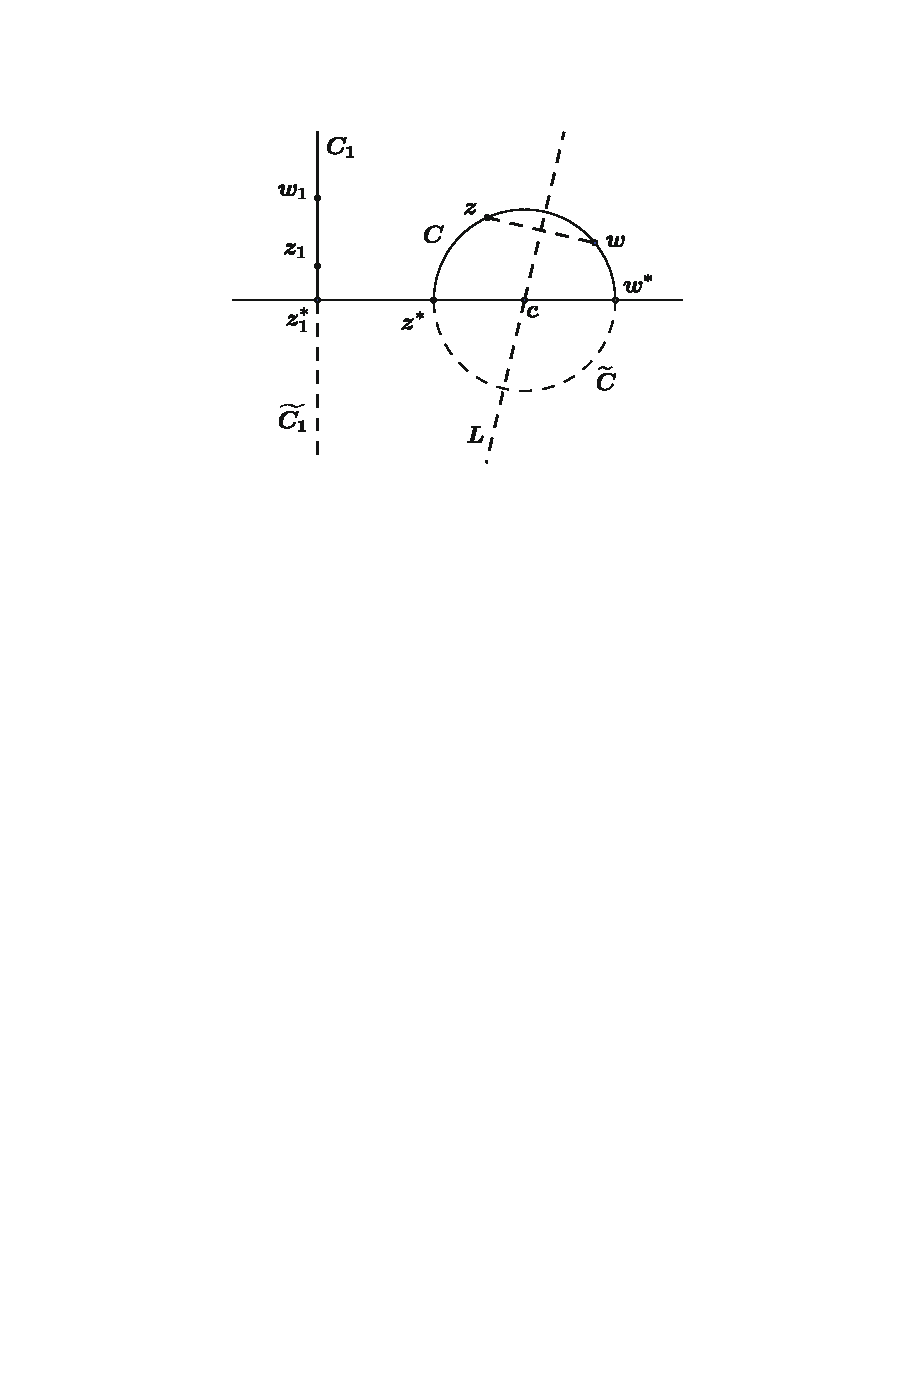
\includegraphics{pictures/upper-plane-conjugate}
\caption{Unique circles (in $\widehat{\C}$) perpendicular to $\R$ through two points in $\mathbb{U}$.}
\end{figure}
\begin{lemma}\label{upper plane change to same re}
Let $z$ and $w$ distinct points in $\mathbb{U}$. There exists a unique $T\in\Aut(\mathbb{U})$ such that $T(z^*)=0$, $T(z)=i$, $T(w)=iy$ with $y>1$, and $T^*(w)=\infty$.
\end{lemma}
\begin{proof}
Consider the unique circle $\widetilde{C}$ centered on the real axis and passing through $z$ and $w$. Since the M\"obius group is triply transitive, there exists a unique M\"obius transformation $T$ that maps $(z^*,w^*,z)$ to $(0,\infty,i)$, respectively. Since M\"obius transformations map circles to circles, $T$ maps $\widetilde{C}$ onto the imaginary axis union $\{\infty\}$, and hence $T(w)=iy$ for some real $y$. Since M\"obius transformations preserve orthogonality of curves, $T$ maps $\R\cup\{\infty\}$ onto itself. Since $T$ maps $z\in\mathbb{U}$ to $i\in\mathbb{U}$, $T$ is in $\Aut(\mathbb{U})$, and because it is orientation preserving, $y>1$.
\end{proof}
\begin{lemma}
If $z$ and $w$ are two distinct points in $\mathbb{U}$, then the hyperbolic length of the geodesic segment $\widetilde{\gamma}$ joining them is shorter than the hyperbolic length of any other piecewise differentiable curve in $\mathbb{U}$ joining them.
\end{lemma}
\begin{proof}
Write $z=x_z+iy_z$ and $w=x_w+iy_w$. First consider the case $x_z=x_w$. Assume the curve $\gamma$ is parameterized by the closed interval $[a,b]\sub\R$ and $\gamma(t)=x(t)+iy(t)$. Then $x$ and $y$ are differentiable functions except at finitely many points, and
\[L_{\mathbb{U}}(\gamma)=\int_{a}^{b}\frac{\sqrt{x'(t)^2+y'(t)^2}}{y(t)}\dif t\geq\int_{a}^{b}\frac{|y'(t)|}{y(t)}\dif t\geq\Big|\log\frac{y_w}{y_z}\Big|=L_{\mathbb{U}}(\widetilde{\gamma}).\]
Furthermore, equality of lengths is attained if and only if $x$ is constant and $y'$ does not change sign where it exists; that is, if and only if $\gamma$ is a reparametrization of $\widetilde{\gamma}$.\par
For the case $x_z\neq x_w$, by Lemma~\ref{upper plane change to same re} we can find a $T$ in $\Aut(\mathbb{U})$ such that $T(z^*)=0$ and $T(w^*)=\infty$. Furthermore, the image under $T$ of the geodesic segment between $z$ and $w$ is the segment on the imaginary axis between $T(z)$ and $T(w)$, and both segments have the same hyperbolic length. Similarly, $T\circ\gamma$ is a piecewise differentiable curve in $\mathbb{U}$ joining $T(z)$ and $T(w)$, with the same hyperbolic length as $\gamma$, and we are reduced to the previous case.
\end{proof}
\begin{theorem}
For any two distinct points $z$ and $w$ in $\mathbb{U}$, the geodesic segment joining $z$ to $w$ is the unique curve that achieves the infimum of $L_{\mathbb{U}}(\gamma)$.
\end{theorem}
Using cross ratios to simplify notation, a routine computation establishes the following result.
\begin{proposition}
For any two distinct points $z$ and $w$ in $\mathbb{U}$, the hyperbolic distance between $z$ and $w$ is equal to the length of the geodesic segment $\gamma$ joining $z$ and $w$, and is given by
\begin{equation}\label{upper plane distance-1}
\begin{aligned}
d_{\mathbb{U}}(z,w)=\log(z,w,w^*,z^*)=\log\frac{|z-\widebar{w}|+|z-w|}{|z-\widebar{w}|-|z-w|}=2\tanh^{-1}\Big(\frac{|z-w|}{|z-\widebar{w}|}\Big).
\end{aligned}
\end{equation}
\end{proposition}
\begin{proof}
We know that the M\"obius transform $T$ in Lemma~\ref{upper plane change to same re} preserve cross ratio, therefore
\[d_{\mathbb{U}}(z,w)=\log y=\log(i,iy,\infty,0)=\log(z,w,w^*,z^*).\]
To show that the cross ratio is given by $(\ref{upper plane distance-1})$, we note that if $\Re(z)=\Re(w)$, then $(\ref{upper plane distance-1})$ reduces to $|\log(y_z/y_w)|$, so in this case the claim is verified. Now we verify that $(\ref{upper plane distance-1})$ is invariant under M\"obious transformations. We only need to consider translation, homothety or inversion. The cases for homothety and translation are clear, and for inversion we have
\[\frac{|z^{-1}-\widebar{w^{-1}}|+|z^{-1}-w^{-1}|}{|z^{-1}-\widebar{w^{-1}}|-|z^{-1}-w^{-1}|}=\frac{\dfrac{|\widebar{w}-z|+|w-z|}{|w||z|}}{\dfrac{|\widebar{w}-z|-|w-z|}{|w||z|}}=\frac{|z-\widebar{w}|+|z-w|}{|z-\widebar{w}|-|z-w|}.\]
Since any pair of points can be send to the imaginary axis by a M\"obious transformation, this proves the claim.
\end{proof}
For interests, we give another formula for the hyperbolic distance of $\mathbb{U}$. This formula generalizes to higher dimensions.
\begin{proposition}
For any two distinct points $z=x_1+iy_1$ and $w=x_2+iy_2$ in $\mathbb{U}$, the hyperbolic distance between $z$ and $w$ is given by
\begin{align}\label{upper plane distance-2}
d_{\mathbb{U}}(z,w)=\cosh^{-1}\Big(1+\frac{(x_1-x_2)^2+(y_1-y_2)^2}{2y_1y_2}\Big).
\end{align}
\end{proposition}
\begin{proof}
Set $p=|z-w|$ and $q=|z-\widebar{w}|$, and let $d=d_{\mathbb{U}}(z,w)$. Then by $(\ref{upper plane distance-1})$ we have
\[\tanh\frac{d}{2}=\frac{p}{q}.\]
By the identity $\cosh^2-\sinh^2=1$, we have $1-\tanh^2=\cosh^{-2}$, therefore
\[\cosh^2\frac{d}{2}=\frac{1}{1-p^2/q^2}=\frac{q^2}{q^2-p^2}.\]
Now with the observation $\cosh(x)=2\cosh^2(x/2)-1$, we then conclude
\begin{align*}
\cosh d&=\frac{2q^2}{q^2-p^2}-1=\frac{q^2+p^2}{q^2-p^2}=\frac{(x_1-x_2)^2+(y_1+y_2)^2+(x_1-x_2)^2+(y_1-y_2)^2}{(x_1-x_2)^2+(y_1+y_2)^2-(x_1-x_2)^2-(y_1-y_2)^2}\\
&=\frac{2((x_1-x_2)^2+(y_1-y_2)^2)+4y_1y_2}{4y_1y_2}=1+\frac{(x_1-x_2)^2+(y_1-y_2)^2}{2y_1y_2}
\end{align*}
or
\[d=\cosh^{-1}\Big(1+\frac{(x_1-x_2)^2+(y_1-y_2)^2}{2y_1y_2}\Big).\]
This proves the claim.
\end{proof}
As mentioned at the end of the previous part, the set $\PSL_2(\R)$ of conformal automorphisms of $\mathbb{U}$ acts as a group of hyperbolic isometries of $\mathbb{U}$. This also follows from two facts: fractional linear transformations preserve the cross ratios and map circles to circles. We now proceed to establish the converse.
\begin{proposition}\label{upper plane isometry fix imaginary axis}
An orientation preserving isometry $f$ of $(\mathbb{U},d_{\mathbb{U}})$ that fixes the imaginary axis pointwise is the identity map.
\end{proposition}
\begin{proof}
Let $z=x+iy$ and $f=u+iv$. For all positive real numbers $t$ we have
\[d(z,it)=d(f(z),f(it))=d(u+iv,it)\]
We calculate using (8.10) that this is equivalent to
\[(x^2+(y-t)^2)(u^2+(v+t)^2)=(x^2+(y+t)^2)(u^2+(v-t)^2)\]
hence also equivalent to
\[(x^2+y^2)v-(u^2+v^2)y=(y-v)t^2\]
for all positive $t$. Since the LHS of the last equation is independent of $t$, the RHS must vanish identically. Hence $v(z)=y$, $u(z)^2=x^2$ and $f(z)=\pm x+iy$. Because $f$ is continuous, the same sign holds for all $z$; thus either $f(z)=z$ or $f(z)=-\widebar{z}$ for all $z$; since $f$ is orientation preserving, we conclude that $f$ is the identity map.
\end{proof}
\begin{theorem}
The set of orientation-preserving isometries of $\mathbb{U}$ with respect to the hyperbolic metric is precisely the set of fractional linear transformations mapping $\mathbb{U}$ to itself; that is, $\PSL_2(\R)$.
\end{theorem}
\begin{proof}
If $g$ is such an isometry of $\mathbb{U}$, it preserves geodesics. Thus there is a fractional linear transformation $f$ that preserves $\mathbb{U}$ and such that $f\circ g$ leaves invariant the imaginary axis. Following this map by an isometry of the form $z\mapsto kz$ with $k>0$ and then (if necessary) by $z\mapsto -z^{-1}$, we may assume that $f\circ g$ fixes $i$ and leaves invariant the intervals $(0,i)$ and $(i,\infty)$ on the imaginary axis. Then we see that $f\circ g$ is the identity on the imaginary axis and hence also on $\mathbb{U}$, by the previous proposition. We conclude that $g$ is a M\"obius transformation.
\end{proof}
\subsubsection{Unit disc model}
Statements about the hyperbolic metric on the upper half plane can be translated to the unit disc model, where the length differential is
\[\lambda_{\D}=\frac{2|\mathrm{d}z|}{1-|z|^2}.\]
We emphasize the following results.
\begin{proposition}
The geodesics in $\D$ are exactly the intersection of a circle with $\D$ whose center is on $\partial\D$.
\end{proposition}
\begin{proof}
The M\"obious transformation $w(z)=(z-i)/(z+i)$ maps the real axis to $\partial\D$, so the claim follows from that of $\mathbb{U}$.
\end{proof}
\begin{proposition}
The set of orientation-preserving isometries of $\D$ consists of the fractional linear transformations mapping $\D$ to itself, that is, $\Aut(\D)$.
\end{proposition}
\begin{proof}
This follows from the observation that if $f:\D\to\D$ is an orientation-preserving isometry, then $w^{-1}\circ f\circ w$ is an orientation-preserving isometry, where $w:\mathbb{U}\to\D$ is given in Corollary~\ref{conformal map from U to D eg}.
\end{proof}
\begin{proposition}
For all $z$ and $w$ in $\D$, the hyperbolic distance is given by
\begin{align}\label{unit disk hyperbolic distance-1}
d_{\D}(z,w)=2\tanh^{-1}\Big(\frac{|z-w|}{|1-\widebar{w}z|}\Big)=\log\frac{|1-\widebar{w}z|+|z-w|}{|1-\widebar{w}z|-|z-w|}.
\end{align}
In particular,
\begin{align}\label{unit disk hyperbolic distance-2}
d_{\D}(0,z)=2\tanh^{-1}(|z|)=\log\frac{1+|z|}{1-|z|}.
\end{align}
\end{proposition}
\begin{proof}
For any points $z_1,z_2\in\D$, we can choose an automorphism $\varphi_{z_1}$ such that $\varphi_{z_1}(z_1)=0$. Then
\[d_{\D}(z_1,z_2)=d_{\D}(0,f(z_2)).\]
Note that $\varphi_{z_1}$ is given by
\[\varphi_{z_1}(z)=\frac{z-z_1}{1-\widebar{z}_1z}.\]
Therefore we only need to check $(\ref{unit disk hyperbolic distance-2})$. We already pointed that the geodesic from $0$ to a point $z\in\D$ is a straight line in $\D$, so
\[d_{\D}(0,z)=\int_{0}^{|z|}\frac{2\dif r}{1-r^2}=\log\frac{1+|z|}{1-|z|}.\]
Thus the claim is proved.
\end{proof}
\subsubsection{Contractions and the Schwarz's lemma}
A deep connection between function theory and geometry is established through Schwarz's lemma. Recall that not every holomorphic self-map of $\D$ is a M\"obius transformation (for instance, $z\mapsto z^2$), only conformal automorphisms are, and, as we have seen, these are isometries in the hyperbolic metric. However, the following result holds.
\begin{theorem}\label{Schwarz lemma generalized}
Holomorphic self-maps of the unit disc do not increase distances with respect to the hyperbolic metric; that is, for all holomorphic self-maps $F$ of $\D$ and all $z$ and $w\in\D$,
\[d_{\D}(F(z),F(w))\leq d_{\D}(z,w)\]
and
\[\lambda_{\D}(F(z))|F'(z)|\leq\lambda_{\D}(z).\]
Furthermore, if for some distinct $z$ and $w$ in $\D$
\[d_{\D}(F(z),F(w))=d_{\D}(z,w)\]
or for some $z\in\D$,
\[\lambda_{\D}|F'(z)|=\lambda_{\D}(z)\]
then $F$ is a conformal self-map of $\D$.
\end{theorem}
\begin{proof}
The two inequalities certainly hold for constant maps $F$. So assume that $F:\D\to\D$ is holomorphic and nonconstant. Assume first that $F(0)=0$. By Schwarz's lemma we have
\[|f(w)|\leq|w|,\quad |f'(0)|\leq 1.\]
These are the Euclidean analogues of the two inequalities in the theorem for the points $z=0$ and arbitrary $w\in\D$. We intend to use equation $(\ref{unit disk hyperbolic distance-2})$ to translate these to the non-Euclidean setting. We start with
\begin{align*}
\frac{1+|F(w)|}{1-|F(w)|}=(1+|F(w)|)\sum_{n=0}^{\infty}|F(w)|^2\leq(1+|w|)\sum_{n=0}^{\infty}|w|^2=\frac{1+|w|}{1-|w|}
\end{align*}
and then apply $(\ref{unit disk hyperbolic distance-2})$ to obtain
\[d_{\D}(0,F(w))\leq d_{\D}(0,w).\]
Let $z_1$ and $z_2$ denote two different points in $\D$; choose conformal automorphisms $\varphi$ and $\psi$ of the unit disc such that $\psi(0)=z_1$ and $\varphi(F(z_1))=0$. Then $\varphi\circ F\circ\psi$ is a holomorphic self-map of the unit disc that fixes $0$. Hence, by what was already established,
\[d_{\D}((\varphi\circ F\circ\psi)(0),(\varphi\circ F\circ\psi)(z))\leq d_{\D}(0,z)\]
for all $z$ in $\D$. Since $\psi$ and $\varphi$ are isometries,
\[d_{\D}((\varphi\circ F\circ\psi)(0),(\varphi\circ F\circ\psi)(z))=d_{\D}((F\circ\psi)(0),(F\circ\psi)(z))\]
and
\[d_{\D}(0,z)=d_{\D}(\psi(0),\psi(z))=d_{\D}(z_1,\psi(z))\]
for all $z$ in $\D$, and we conclude that
\[d_{\D}(F(z_1),F(\psi(z)))\leq d_{\D}(z_1,\psi(z)).\]
Taking $\psi(z)=z_2$, we then get
\begin{align}\label{Schwarz lemma generalized-1}
d_{\D}(F(z_1),F(z_2))\leq d_{\D}(z_1,z_2).
\end{align}
If we multiply each side of the last equation by
\[\Big|\frac{1}{z_1-z_2}\Big|=\Big|\frac{1}{F(z_1)-F(z_2)}\cdot\frac{F(z_1)-F(z_2)}{z_1-z_2}\Big|\]
and take the limit as $z_1$ approaches $z_2$, we get the infinitesimal form of our required formula (the second inequality)
\begin{align}\label{Schwarz lemma generalized-2}
\lambda_{\D}(F(z_2))\leq|F'(z_2)|\lambda_{\D}(z_2).
\end{align}
If one of the equality in either $(\ref{Schwarz lemma generalized-1})$ or $(\ref{Schwarz lemma generalized-2})$ holds, then as in the proof of Schwarz lemma, we conclude that $\varphi\circ F\circ\psi$ is a rotation, so that $F$ is a conformal map.
\end{proof}
\begin{definition}
Let $X$ be a metric space with distance $d$. A self-map $f$ of $X$ is a \textbf{contraction} if $d(f(x),f(y))<d(x,y)$ for all $x$ and $y$ in $X$ with $x\neq y$.
\end{definition}
Theorem~\ref{Schwarz lemma generalized} can be restated as
\begin{theorem}
A holomorphic self-map of the unit disc is either an isometry or a contraction with respect to the hyperbolic metric.
\end{theorem}
\subsection{Finite Blaschke products}
For $a\in\D$, set
\[B_{a}(z)=-\frac{|a|}{a}\frac{z-a}{1-\widebar{a}z}\]
for $z\in\C$, with the understanding that $|a|/a=1$ if $a=0$.  Of course, $B_a$ is the Riemann map $f$ for $\D$ normalized (as before) by sending $a$ to $0$ but with (the change that) $\arg f'(0)=\pi-\arg a$; it is an automorphism of $\D$.\par
Let $A=\{a_0,a_1,\dots\}$ be a nonempty finite or countable sequence of complex numbers lying in the unit disc $\D$. Define
\[B(z)=B_A(z)=\prod_{i}B_{a_i}(z)\]
\begin{definition}
The function $B_A$ is the (finite or infinite) \textbf{Blaschke product} associated to $A$. In the infinite case there are, of course, convergence issues.
\end{definition}
For the rest we will study finite Blaschke products. It follows immediately from the definition that we have
\begin{proposition}
If $A=\{a_0,\dots,a_n\}$ is a nonempty finite sequence of points in $\D$, then
\begin{itemize}
\item[(a)] $B=B_A$ is a meromorphic function on $\widehat{\C}$, with zeros precisely at the $n+1$ points $\{a_i\}$ and poles at the $n+1$ points $\{1/\widebar{a}_i\}$.
\item[(b)] $B$ is a self-map of the closed unit disc, that maps the open unit disc holomorphically onto itself, and the unit circle onto itself, with $B(0)=\prod_i|a_i|$.
\end{itemize}
\end{proposition}
Blaschke products transform beautifully under automorphisms of $\D$, as shown next.
\begin{proposition}\label{Blaschke product compose auto of D}
Let $A=\{a_0,\dots,a_n\}$ be a nonempty finite sequence of points in $\D$, and let $T$ be any element of $\Aut(\D)$. Then
\[B_A\circ T=\lambda B_{T^{-1}(A)},\]
where $\lambda$ is a constant of absolute value $1$.
\end{proposition}
\begin{proof}
Since $T$ belongs to $\Aut(\D)$, there exist $\alpha\in\R$ and $a\in\D$ such that
\[T(z)=e^{i\alpha}\frac{z-a}{1-\widebar{a}z}\]
for all $z$ in $\D$. It suffices to compute the action of $T$ on the function $z\mapsto(z-c)/(1-\widebar{c}z)$, where $c\in\D$. A calculation shows that
\begin{align*}
\frac{T(z)-c}{1-\widebar{c}T(z)}&=\frac{e^{i\alpha}\frac{z-a}{1-\widebar{a}z}-c}{1-\widebar{c}e^{i\alpha}\frac{z-a}{1-\widebar{a}z}}=\frac{e^{i\alpha}(z-a)-c(1-\widebar{a}z)}{1-\widebar{a}z-\widebar{c}e^{i\alpha}(z-a)}=\frac{(\widebar{a}c+e^{i\alpha})z-(ae^{i\alpha}+c)}{(1+\widebar{c}e^{i\alpha}a)-(\widebar{a}+\widebar{c}e^{i\alpha}z)}\\
&=\frac{\widebar{a}c+e^{i\alpha}}{1+\widebar{c}e^{i\alpha}a}\cdot\frac{z-\frac{ae^{i\alpha}+c}{\widebar{a}c+e^{i\alpha}}}{1-\frac{\widebar{a}+\widebar{c}e^{i\alpha}}{1+\widebar{c}e^{i\alpha}a}z}=\frac{\widebar{a}c+e^{i\alpha}}{e^{i\alpha}(a\widebar{c}+e^{-i\alpha})}\cdot\frac{z-\frac{ae^{i\alpha}+c}{\widebar{a}c+e^{i\alpha}}}{1-\frac{\widebar{a}e^{-i\alpha}+\widebar{c}}{a\widebar{c}+e^{-i\alpha}}z}\\
&=\frac{\widebar{a}c+e^{i\alpha}}{e^{i\alpha}\widebar{(\widebar{a}c+e^{i\alpha})}}\cdot\frac{z-\frac{ae^{i\alpha}+c}{\widebar{a}c+e^{i\alpha}}}{1-\widebar{\Big(\frac{ae^{i\alpha}+c}{\widebar{a}c+e^{i\alpha}}\Big)}z}=\frac{\widebar{a}c+e^{i\alpha}}{e^{i\alpha}\widebar{(\widebar{a}c+e^{i\alpha})}}\cdot\frac{z-T^{-1}(c)}{1-\widebar{T^{-1}(c)}z}.
\end{align*}
The proof is completed by observing that $|(\widebar{a}c+e^{i\alpha})/(e^{i\alpha}\widebar{(\widebar{a}c+e^{i\alpha})})|=1$ and that
\[T^{-1}(w)=\frac{ae^{i\alpha}+w}{w\widebar{a}+e^{i\alpha}}.\]
Thus the claim follows.
\end{proof}
\begin{theorem}\label{Blaschke product prop}
Let $f$ be a holomorphic self-map of the open unit disc $\D$, $A=\{a_0,a_1,\dots,a_n\}$ a nonempty finite collection of points in $\D$ and $B=B_A$. Assume that $f(a_i)=0$ for each $a_i$ in $A$, with multiplicities; that is, $\nu_{a_i}(f)\geq\nu_{a_i}(B)$ for all $i$. Then
\begin{itemize}
\item[(a)] $|f(z)|\leq|B(z)|$ for all $z\in\D$, and $|f'(a_i)|\leq|B'(a_i)|$ for all $i=1,\dots,n$.
\item[(b)] If $|f(a)|=|B(a)|$ for some $a\in\D$ with $a\neq a_i$ for all $i$, then there is $\alpha\in\R$ such that $f(z)=e^{i\alpha}B(z)$.
\item[(c)] If $a_i$ appears $\nu$ times in the sequence $A$ and if
\[0=f(a_i)=\cdots=f^{(\nu-1)}(a_i)\quad\text{and}\quad|f^{(\nu)}(a_i)|=|B^{(\nu)}(a_i)|\]
then there exists $\alpha\in\R$ such that $f(z)=e^{i\alpha}B(z)$.
\end{itemize}
\end{theorem}
\begin{proof}
Consider the function
\[F(z)=\frac{f(z)}{B(z)}\]
on $\D$. Since $\nu_{a_i}(f)\geq\nu_{a_i}(B)$, the points $a_i$ in $A$ are all removable singularities of $F$, and we can extend $F$ to a holomorphic function on $\D$, which is still denoted by $F$. In view of the definition of $F(z)$, it suffices to show that $|F(z)|\leq 1$ for $z\in\D$. Fix such a point $z$. The restrictions of $|B|$ to circles of radius $r$, with $0\leq r\leq 1$, yield a family of functions that uniformly approach the constant function $1$ as $r$ approaches $1$. Hence, for all $\eps>0$, we can choose an $r$ such that $|B(w)|\geq 1-\eps$ for $|w|=r$. Without loss of generality we may assume that $r\geq|z|$. Hence, by the maximum principle for $|w|\leq r$, it follows that
\[|F(w)|=\frac{|f(w)|}{|B(w)|}\leq\frac{1}{(1-\eps)}.\]
Since $\eps$ is arbitrary and the inequality holds for all $|z|\leq r<1$, the claim is proved.\par
To prove (b) and (c), we first note that the function $F(z)=f(z)/B(z)$ is holomorphic on $\D$ with modulus as most $1$, and the value of $F$ on $A$ is obtained by defining
\[F(a_i):=\lim_{z\to a_i}\frac{f(z)}{B(z)}=\frac{f^{(\nu_i)}(a_i)}{B^{(\nu_i)}(a_i)}.\]
where $\nu_i=\nu_{a_i}(B)$. Thus if $|f(a)|/|B(a)|=1$ for some $a\in\D\setminus A$ or $|f^{(\nu_i)}(a_i)|=|B^{(\nu_i)}(a_i)|$, then the modulus of $f/B$ obtain its maximum in $\D$, and by maximal modulus principle $F$ is constant.
\end{proof}
The particular case when $A$ consists of one point leads to the following interesting result, a generalization of Schwarz's lemma.
\begin{corollary}[\textbf{Schwarz-Pick Lemma}]
Let $f$ be a holomorphic self-map of the open unit disc $\D$. If $a\in\D$, then for any $z\in\D$
\[\frac{f(z)-f(a)}{1-\widebar{f(a)}f(z)}\leq\frac{|z-a|}{|1-\widebar{a}z|}\quad\text{and}\quad|f'(a)|\leq\frac{1-|f(a)|^2}{1-|a|^2}.\]
Furthermore, equality for one $z\neq a$ in the first inequality or equality in the second inequality implies that $f$ is an automorphism of $\D$.
\end{corollary}
\begin{proof}
Apply the previous theorem to the function $B_{f(a)}\circ f$.
\end{proof}
This corollary may also be deduced by applying Schwarz's lemma to the function $B_{f(a)}\circ f\circ B_a^{-1}$ or, more interesting, is equivalent to Theorem~\ref{Schwarz lemma generalized}.
\section{Harmonic functions}
\subsection{Harmonic functions and the Laplacian}
We begin with the Laplace operator.
\begin{definition}
Let $D$ be a domain in $\C$ and $g\in C^2(D)$. We define $\Delta g$, the \textbf{Laplacian} of $g$, by
\[\Delta g=\frac{\partial^2g}{\partial x^2}+\frac{\partial^2g}{\partial y^2}.\]
The operator $\Delta$ is also called the \textbf{Laplacian} or the \textbf{Laplace operator}. If $D$ is a domain in $\C$ and $g\in C^2(D)$, we say that $g$ is harmonic in $D$ if it satisfies \textbf{Laplace's equation} $\Delta g=0$ in $D$.
\end{definition}
The last two definitions have a number of immediate consequences:
\begin{itemize}
\item It is obvious from the definition of the Laplacian as a linear operator on $C^2$ complex-valued functions that it preserves real-valued functions. It is useful to have equivalent formulae for it
\begin{align}\label{Laplacian in complex coordinate}
\Delta=\frac{\partial^2}{\partial x^2}+\frac{\partial^2}{\partial y^2}=4\frac{\partial^2}{\partial z\partial\widebar{z}}=4\frac{\partial^2}{\partial\widebar{z}\partial z}
\end{align}
and in polar coordinates
\begin{align}\label{Laplacian in polar coordinate}
\Delta=\frac{1}{r}\frac{\partial}{\partial r}\Big(r\frac{\partial}{\partial r}\Big)+\frac{1}{r}\frac{\partial}{\partial\theta}\Big(\frac{1}{r}\frac{\partial}{\partial\theta}\Big)=\frac{1}{r}\frac{\partial^2}{\partial r^2}+\frac{1}{r}\frac{\partial}{\partial r}+\frac{1}{r^2}\frac{\partial^2}{\partial\theta}.
\end{align}
\item Recall that for $f\in C^1(D)$, $f$ is holomorphic on $D$ if and only if $\partial f/\partial\widebar{z}=0$ in $D$. Thus, for $g\in C^2(D)$, $g$ is harmonic if and only if $\partial g/\partial z$ is holomorphic. In particular, holomorphic functions are harmonic and this gives an easy way to construct analytic functions from harmonic ones.
\item $f$ is harmonic if and only if $\widebar{f}$ is. In fact, we have
\[\Delta\widebar{f}=\widebar{\Delta f}.\]
\item $f$ is harmonic if and only if $\Re(f)$ and $\Im(f)$ are. This follows from the linearity of $\Delta$.
\item If $f$ is holomorphic on an open set $D$, then $f$, $\Re(f)$, $\Im(f)$, and $f$ are harmonic on $D$.
\item If $f$ is holomorphic or anti-holomorphic on $D$ and $g$ is harmonic on $f(D)$, then $g\circ f$ is harmonic on $D$. This follows from the chain rule: Assume that $f$ is holomorphic, and let $w=g(z)$, then
\[(g\circ f)_{z}=g_wf_z+g_{\widebar{w}}\widebar{f}_z=g_wf_z\]
and
\[(g\circ f)_{z\widebar{z}}=(g_wf_z)_{\widebar{z}}=g_{ww}f_{\widebar{z}}f_{z}+g_{w\widebar{w}}\widebar{f}_{\widebar{z}}f_z+g_{w}f_{z\widebar{z}}=0.\]
The argument in the anti-holomorphic case is similar.
\item If $f\in C^2(D)$ and $f$ is locally on $D$ the real part of an analytic function, then $f$ is harmonic on $D$.
\end{itemize}
\begin{example}
The function $\log|z|$ is harmonic on $D=\C^*$, since it belongs to $C^2(D)$, and it is locally the real part of $\log z$, a multi-valued but holomorphic function in $D$.
\end{example}
\begin{proposition}\label{harmonic function is real part}
If $g$ is real-valued and harmonic in $D$, then it is locally the real part of an analytic function. The analytic function is unique up to an additive constant.
\end{proposition}
\begin{proof}
Let $\Omega\sub D$ be a simply connected region. Since $g$ is harmonic in $\Omega$, it follows that $2g_{z}dz$ is closed on $\Omega$, and hence an exact form on $\Omega$. Choose a holomorphic function $f$ on $\Omega$ with $df=2g_z\dif z$. Then
\[d\widebar{f}=2g_{\widebar{z}}\dif\widebar{z}\]
and hence
\[\frac{1}{2}d(f+\widebar{f})=g.\]
This means $g=\Re(f)+\text{constant}$ on $\Omega$.
\end{proof}
\begin{corollary}
A real-valued harmonic function on a simply connected domain is
the real part of a holomorphic function on the same domain.
\end{corollary}
\begin{corollary}
A harmonic function is $C^\infty$.
\end{corollary}
\begin{corollary}
Harmonic functions have the MVP, and hence they satisfy the maximum modulus principle. Real-valued harmonic functions also satisfy the maximum and minimum principles.
\end{corollary}
\begin{remark}
The maximum (minimum) principle asserts that if $f$ is real-valued and harmonic on a domain $D$ and if $f$ has a relative maximum (minimum) at a point $z_0\in D$, then $f$ is constant in a neighborhood of $z_0$. Furthermore, if $D$ is bounded and if $f$ is also continuous on the closure of $D$, with $m\leq f\leq M$ on $\partial D$ for some real constants $m$ and $M$, then $m\leq f\leq M$ on $D$.
\end{remark}
\subsection{Integral representation of harmonic functions}
We apply the Cauchy theory towards our present main goal, which is to solve a boundary value problem. Given a harmonic function defined in a disc, we derive an integral formula for it, known as the Poisson formula; a major tool in the solution of our boundary value problem.
\begin{proposition}[\textbf{The Poisson Formula}]
If $g$ is a harmonic function on the domain $|z|<\rho$ for some $\rho>0$, then, for each $0<r<\rho$,
\begin{align}\label{Possion formula}
g(z)=\frac{1}{2\pi i}\int_{0}^{2\pi}g(re^{i\theta})\cdot\frac{r^2-|z|^2}{|re^{i\theta}-z|^2}\dif\theta\quad\text{for }|z|<r.
\end{align}
\end{proposition}
\begin{proof}
It suffices to assume that $g$ is real-valued. To establish this formula we can thus apply Proposition~\ref{harmonic function is real part} and choose the holomorphic function $f$ on this domain with $\Re(f)=g$ and $g(0)=f(0)$, noting that there is a unique such $f$.\par
Since $f$ is holomorphic in the disk $|z|<\rho$, it has a power series expansion $f(z)=\sum_{n=0}^{\infty}a_nz^n$, and therefore
\[g(z)=\frac{f(z)+\widebar{f(z)}}{2}=\frac{1}{2}\sum_{n=0}^{\infty}(a_nz^n+\widebar{a}_n\widebar{z}^n).\]
Now we determine the coefficients $a_n$. Set $z=re^{i\theta}$ in the above expression, we get
\[g(re^{i\theta})=a_0+\frac{1}{2}\sum_{n=1}^{\infty}r^n(a_ne^{in\theta}+\widebar{a}_ne^{-in\theta}).\]
Multiplying by $e^{-in\theta}$ and integrating along the curve $|z|=r$ yields
\[a_0=\frac{1}{2\pi}\int_{0}^{2\pi}g(re^{i\theta})\dif\theta,\quad a_n=\frac{1}{\pi}\int_{0}^{2\pi}\frac{g(re^{i\theta})}{(re^{i\theta})^n}\dif\theta.\]
Thus, for $|z|<r$, we obtain that
\begin{align*}
f(z)&=\frac{1}{2\pi}\int_{0}^{2\pi}g(re^{i\theta})\Big[1+2\sum_{n=1}^{\infty}\Big(\frac{w}{re^{i\theta}}\Big)^n\Big]\dif\theta=\frac{1}{2\pi}\int_{0}^{2\pi}g(re^{i\theta})\Big[1+2\sum_{n=1}^{\infty}\Big(\frac{z}{re^{i\theta}}\Big)^n\Big]\dif\theta\\
&=\frac{1}{2\pi}\int_{0}^{2\pi}g(re^{i\theta})\frac{re^{i\theta}+z}{re^{i\theta}-z}\dif\theta.
\end{align*}
The last formula gives a representation of a holomorphic function $f$ in terms of its real part $g$, when the function $f$ is real at $0$. Taking the real part of both sides we obtain equation $(\ref{Possion formula})$, the Poisson formula.
\end{proof}
The function
\[\Re\Big(\frac{re^{i\theta}-z}{re^{i\theta}+z}\Big)=\frac{r^2-|z|^2}{|re^{i\theta}-z|^2}\]
is known as the \textbf{Poisson kernel}.\par
The original derivation of formula $(\ref{Possion formula})$ assumed that $g$ was harmonic in the closed disc $\{z:|z|\leq r\}$. However, the result remains true for $|z|<r$ under the weaker assumption that $g$ is harmonic in the open disc $|z|<r$ and continuous on its closure. In this case, fix $t$ with $0<t<1$ and look at the function of $z$ given by $g(tz)$. It is harmonic on the closed disc $\{z:|z|\leq r\}$ and hence, by the already proven formula $(\ref{Possion formula})$,
\[g(tz)=\frac{1}{2\pi}\int_{0}^{2\pi}g(rte^{i\theta})\frac{r^2-|z|^2}{|rte^{i\theta}-z|^2}\dif\theta.\]
Since the function $g$ is uniformly continuous on the closed disc, we know that $g(tz)$ approaches $g(z)$ uniformly on the circle $\{z:|z|=r\}$ as $t$ approaches $1$. Hence both sides of the last equation converge to the expected quantities.\par
As a special case we apply the Poisson formula to the function $g$ which is identically $1$ and obtain
\[\frac{1}{2\pi}\int_{0}^{2\pi}\frac{r^2-|z|^2}{|re^{i\theta}-z|^2}\dif\theta=1.\]
\begin{definition}
A harmonic conjugate of a real-valued harmonic function $u$ is any real-valued function $v$ such that $u+iv$ is holomorphic.
\end{definition}
Harmonic conjugates always exist locally, and globally on simply connected domains. They are unique up to additive real constants. In fact, it is easy to see that they are given locally as follows.
\begin{proposition}
If $g$ is harmonic and real-valued in $|z|<\rho$ for some $\rho>0$, then the harmonic conjugate of $g$ vanishing at the origin is given by
\[\frac{1}{2\pi i}\int_{0}^{2\pi}g(re^{i\theta})\frac{re^{-i\theta}z-re^{i\theta}\widebar{z}}{|re^{i\theta}-z|^2}\dif\theta\]
for $0<r<\rho$.
\end{proposition}
The following result is interesting and useful.
\begin{theorem}[\textbf{Harnack's Inequalities}]
If $g$ is a positive harmonic function on $|z|<r$ that is continuous on $|z|<r$, then
\[\frac{r-|z|}{r+|z|}\cdot g(0)\leq g(z)\leq\frac{r+|z|}{r-|z|}\cdot g(0)\quad\text{for all $|z|<r$}.\]
\end{theorem}
\begin{proof}
Our starting point is $(\ref{Possion formula})$. We use elementary estimates for the Poisson kernel:
\[\frac{r-|z|}{r+|z|}=\frac{r^2-|z|^2}{(r+|z|)^2}\leq\frac{r^2-|z|^2}{|re^{i\theta}-z|^2}\leq\frac{r^2-|z|^2}{(r-|z|)^2}=\frac{r+|z|}{r-|z|}.\]
Multiplying these inequalities by the positive number $g(w)=g(re^{i\theta})$ and then averaging the resulting function over the circle $|w|=r$, we obtain
\begin{align*}
\frac{r-|z|}{r+|z|}\cdot\frac{1}{2\pi}\int_{0}^{2\pi}g(re^{i\theta})\dif\theta\leq\frac{1}{2\pi}\int_{0}^{2\pi}g(re^{i\theta})\frac{r^2-|z|^2}{|re^{i\theta}-z|^2}\dif\theta\leq\frac{r+|z|}{r-|z|}\cdot\frac{1}{2\pi}\int_{0}^{2\pi}g(re^{i\theta})\dif\theta.
\end{align*}
The middle term in the above inequalities is $g(z)$ as a consequence of $(\ref{Possion formula})$, while the extreme averages are equal to $g(0)$ by the MVP.
\end{proof}
\begin{corollary}\label{Harnack's Inequality compact set}
Let $K$ be a compact subset of a domain $D\sub\C$, and let $u$ be a positive harmonic function on $D$. Then there exists a constant $C>1$ that depends only on $K$ and $D$, but not on $u$, such that
\[C^{-1}\leq\frac{u(z_1)}{u(z_2)}\leq C\]
for all $z_1,z_2\in K$.
\end{corollary}
\begin{proof}
Since $u$ is positive, by Harnack's Inequality we have
\[\frac{(r-|z_1|)(r-|z_2|)}{(r+|z_1|)(r+|z_2|)}\leq\frac{u(z_1)}{u(z_2)}\leq\frac{(r+|z_1|)(r+|z_2|)}{(r+|z_1|)(r+|z_2|)}\]
for $z_1,z_2\in K\cap B_{r}(z_0)$, where $z_0$ is a fixed point in $K$. Since $K$ is compact, there exist a $\delta>0$ such that $B_{\delta}(z_0)\sub D$ for any $z_0\in K$. Then it is easy to see the claim.
\end{proof}
\begin{theorem}[\textbf{Harnack's Convergence Theorem}]
Let $D$ be a domain and let $\{u_n\}$ be a nondecreasing sequence of real-valued harmonic functions on $D$. Then
\begin{itemize}
\item[(a)] Either $\lim_nu_n(z)=+\infty$ for all $z\in D$, or
\item[(b)] The function on $D$ defined by $u(z)=\lim_nu_n(z)$ is harmonic in $D$.
\end{itemize}
\end{theorem}
\begin{proof}
Since a nondecreasing sequence of real numbers converges if and only if it is bounded, the assumption that $\lim_nu_n(z)$ is not $+\infty$ for all $z\in D$ allows us to conclude that there exist $z_0$ in $D$ and a real number $M$ such that $u(z_0)\leq M$ for all $n$. Then $\lim_nu_n(z_0)$ exists, and it equals the value of the series
\[u_1(z_0)+\sum_{n=1}^{\infty}[u_{n+1}(z_0)-u_n(z_0)].\]
which is therefore convergent.\par
Let $K$ denote a compact subset of $D$. By enlarging $K$ if necessary, we may assume that $z_0\in K$. It follows from Corollary~\ref{Harnack's Inequality compact set} that there exists a real constant $C$ such that
\[0\leq u_{n+1}(z)-u_n(z)\leq C[u_{n+1}(z)-u_n(z)]\]
for all $z$ in $K$ and all $n>0$. It follows immediately that the series $u_1(z)+\sum_{n}[u_{n+1}(z)-u_n(z)]$ converges uniformly on $K$; that is, $u_n$ converges uniformly to a function $u$ on compact subsets of $D$. It is noweasy to showthat $u$ is harmonic in $D$.
\end{proof}
\subsection{The Dirichlet problem}
Let $D$ be a bounded region in $\C$ and let $f\in C(\partial D)$. The Dirichlet problem is to find a continuous function $u$ defined on the closure of $D$ that agrees with $f$ on the boundary of $D$ and whose restriction to $D$ is harmonic. We will consider, for the moment, only the special case where $D$ is a disc; without loss of generality we may assume that the disc has radius one and center at zero.\par
For a piecewise continuous function $u$ on $S^1$ and $z\in\C$ with $|z|<1$, we define (compare with $(\ref{Possion formula})$)
\[P[u](z)=\frac{1}{2\pi}\int_{0}^{2\pi}u(e^{i\theta})\frac{1-|z|^2}{|e^{i\theta}-z|^2}\dif\theta.\]
The following properties of the operator $P$ are easily established.
\begin{itemize}
\item[(a)] $P[u]$ is a well-defined function on the open unit disc. Hence we view $P$ as an operator that assigns the function $P[u]$, on the open unit disc to each piecewise continuous function $u$ on the unit circle.
\item[(b)] $P[u+v]=P[u]+P[v]$ and $P[cU]=cP[u]$ for all piecewise continuous functions $u$ and $v$ on $S^1$ and every constant $c$.
\item[(c)] If $u$ is a real nonnegative piecewise continuous function on $S^1$, then $P[u]$ is a real-valued nonnegative function on the open unit disc.
\item[(d)] $P[u]$ is harmonic in the open unit disc.
\item[(e)] Any bound on $u$ yields the same bound on $P[u]$. For example, for real-valued function $u$ satisfying $m\leq u\leq M$ for some real constants $m$ and $M$, we have $m\leq P[u]\leq M$.
\end{itemize}
We now establish the solvability of the Dirichlet problem for discs.
\begin{theorem}[\textbf{H. A. Schwarz}]
If $u$ is a piecewise continuous function on the unit circle $S^1$, then the function $P[u]$ is harmonic on the unit disk; furthermore, for $\theta\in\R$, its limit as $z$ approaches $e^{i\theta}$ is $u(e^{i\theta})$ provided $u$ is continuous at $e^{i\theta}$. In particular, the Dirichlet problem is solvable for discs.
\end{theorem}
\begin{proof}
We only have to study the boundary values for $P[u]$. Let $C_1$ and $C_2$ be complementary arcs on the unit circle. Let $u_1$ be the function which coincides with $u$ on $C_1$ and vanishes on $C_2$; let $u_2$ be the corresponding function for $C_2$. Clearly $P[u]=P[u_1]+P[u_2]$. The function $P[u_1]$ can be regarded as an integral over the arc $C_1$; hence it is harmonic on $\C\setminus C_1$. The expression
\[\Re\Big(\frac{e^{i\theta}+z}{e^{i\theta}-z}\Big)=\frac{1-|z|^2}{|e^{i\theta}-z|^2}.\]
vanishes on $|z|=1$ for $z\neq e^{i\theta}$. It follows that $P[u_1]$ is zero on the one-dimensional interior of the arc $C_2$. By continuity $P[u_1]$ approaches zero as $z$ approaches a point in the interior of $C_2$.\par
In proving that $P[u]$ has limit $u(e^{i\theta_0})$ at $e^{i\theta_0}$, we may assume that $u(e^{i\theta_0})=0$. Under this assumption, given an $\eps>0$, we can find complementary arcs $C_1$ and $C_2$ on the unit circle such that $e^{i\theta}$ is an interior point of $C_2$ and $|u(e^{i\theta})|\leq\eps/2$ for $e^{i\theta}\in C_2$. This last condition implies that $|u_2(e^{i\theta})|<\eps/2$ for all $e^{i\theta}$, and hence $|P[u_2](z)|\leq\eps/2$ for all $|z|<1$.\par
But we also have that $u_1$ is continuous and vanishes at $e^{i\theta_0}$. Since $P[u_1]$ is continuous at $e^{i\theta_0}$ and agrees with $u_1$ there, there exists a $\delta>0$ such that $|P[u_1](z)|<\eps/2$ for $|z-e^{i\theta_0}|<\delta$. It follows that
\[|P[u](z)|\leq|P[u_1](z)|+|P[u_2](z)|<\eps.\]
as long as $|z|<1$ and $|z-e^{i\theta_0}|<\delta$. This is the required continuity statement.
\end{proof}
As an application, we use the solution of Dirichlet problem to prove the characterization of harmonic functions.
\begin{theorem}
A continuous complex-valued function that satisfies the MVP is harmonic.
\end{theorem}
\begin{proof}
Let $f$ be a continuous function on a domain $D$, let $z_0\in D$ and let $r_0>0$ be sufficiently small so that $\widebar{B_{r_0}(z_0)}\sub D$ and $f$ satisfies MVP for all $r<r_0$. It suffices to assume that $f$ is real-valued. Let $v$ be the continuous function on $\widebar{B_{r_0}(z_0)}$ that is harmonic on $B_{r_0}(z_0)$ and agrees with $f$ on $\partial B_{r_0}(z_0)$. Then $f-v$ has the MVP in $B_{r_0}(z_0)$, and thus attains its maximum and minimum on $\partial B_{r_0}(z_0)$. Since $f-v=0$ on $\partial B_{r_0}(z_0)$, we conclude that $f\equiv v$ on $B_{r_0}(z_0)$ and thus that $f$ is harmonic there.
\end{proof}
\subsubsection{Fourier series interpretation of the Poisson formula}
We again consider the case of the unit disc and proceed to compute the power series expansion of $P[u](z)$ at the origin. Noting that
\[P[u](z)=\frac{1}{2\pi}\int_{0}^{2\pi}\frac{1-z\widebar{z}}{(e^{i\theta}-z)(e^{-i\theta}-\widebar{z})}\dif\theta.\]
We start with an expansion of the Poisson kernel
\begin{align*}
\frac{1-z\widebar{z}}{(e^{i\theta}-z)(e^{-i\theta}-\widebar{z})}&=\frac{1-z\widebar{z}}{(1-e^{-i\theta}z)(1-e^{i\theta}\widebar{z})}=(1-z\widebar{z})\sum_{n,m=0}^{\infty}e^{-in\theta}z^n\cdot e^{im\theta}\widebar{z}^m\\
&=(1-z\widebar{z})\sum_{n,m=0}^{\infty}e^{i(m-n)\theta}z^n\widebar{z}^m\\
&=\sum_{n,m=0}^{\infty}e^{i(m-n)\theta}z^n\widebar{z}^m-\sum_{n,m=1}^{\infty}e^{i(m-n)\theta}z^n\widebar{z}^m\\
&=1+\sum_{n=1}^{\infty}e^{in\theta}z^n+\sum_{m=1}^{\infty}e^{-im\theta}\widebar{z}^m.
\end{align*}
and since the last two series converge uniformly and absolutely on all compact subsets of the unit disc, we conclude
\begin{align}\label{Possion formula fourier interpretation}
P[u](z)=a_0+\sum_{n=1}^{\infty}a_nz^n+\sum_{m=1}^{\infty}b_m\widebar{z}^m.
\end{align}
where, for $n>0$ and $m>0$,
\[a_n=\frac{1}{2\pi}\int_{0}^{2\pi}u(e^{i\theta})e^{-in\theta}d\dif\theta,\quad b_m=\frac{1}{2\pi}\int_{0}^{2\pi}u(e^{i\theta})e^{in\theta}\dif\theta.\]
We thus have the following procedure for extending a given continuous function $u$ on the unit circle to a continuous function on the closed unit disc that is harmonic on the interior of the disc. First compute the Fourier series of $u$:
\[u(e^{i\theta})=a_0+\sum_{n=1}^{\infty}a_ne^{in\theta}+\sum_{m=1}^{\infty}b_me^{-im\theta}.\]
In this series replace $e^{in\theta}$ by $z^n$ and $e^{-im\theta}$ by $\widebar{z}^m$.
\subsubsection{Classical reformulation of the Poisson formula}
For the next reformulation, we start with
\begin{definition}
If $\omega=P\dif x+Q\dif y$ is a differential form, we define $^{\ast}\omega$, the \textbf{conjugate differential} of $\omega$, by
\[^{\ast}\omega=-Q\dif x+P\dif y.\]
\end{definition}
It turns out that the conjugate differential has intense connection with conjugate harmonic functions.
\begin{proposition}\label{conjugate differential is harmonic conjugate}
Suppose that $D$ is a simply connected domain and $u\in C^2(D)$ is real-valued. If $u$ is harmonic and $v$ is harmonic conjugate of $u$, then
\[^{\ast}du=dv.\]
In particular, the conjugate differential $^{\ast}du$ is exact.
\end{proposition}
\begin{proof}
We know that $u$ is harmonic on $D$ if and only if $u$ is the real part of an analytic function $f$ on $D$. In this case,
\begin{align*}
df&=f'(z)\dif z=(u_x-iu_y)(\dif x+i\dif y)\\
&=(u_x\dif x+u_y\dif y)+i(-u_y\dif x+u_x\dif y)\\
&=du+i\,{^{\ast}du}.
\end{align*}
Thus the claim follows.
\end{proof}
In what follows we work with cycles rather than curves. In the general case, for a harmonic function $u$ on an arbitrary domain $D$, the form $du=u_x\dif x+u_y\dif y$ is clearly exact on $D$, and its conjugate differential $^{\ast}du=-u_y\dif x+u_x\dif y$ is closed since $u_{xx}+u_{yy}=0$. We conclude that
\begin{align}\label{integral of conjugate form}
\int_{\gamma}{^{\ast}du}=0
\end{align}
for all harmonic functions $u$ on $D$ and all cycles $\gamma$ in $D$ that are homologous to zero on that domain.\par
Assume that $\gamma$ is a regular curve with equation $z=z(t)$. The direction of the tangent line to the curve at $z(t)$ is determined by the angle $\alpha=\arg z'(t)$ and
\[\dif x=|\mathrm{d}z|\cos\alpha,\quad \dif y=|\mathrm{d}z|\sin\alpha.\]
The normal line at $z(t)$, which points to the right of the tangent line, has direction $\beta=\alpha-\pi/2$. The \textbf{normal derivative} of $u$ is the directional derivative of $u$ in the direction $\beta$:
\[\frac{\partial u}{\partial n}=u_x\cos\beta+u_y\sin\beta=u_x\sin\alpha-u_y\cos\alpha.\]
Thus we see that $^{\ast}du=(\partial u/\partial n)|\mathrm{d}z|$, and $(\ref{integral of conjugate form})$ can be rewritten as
\[\int_{\gamma}\frac{\partial u}{\partial n}|\mathrm{d}z|=0.\]
It is important to realize that if $\gamma$ is the circle $|z|=r$, then $\partial u/\partial n=\partial u/\partial r$.
\begin{theorem}
If $u_1$ and $u_2$ are harmonic functions on $D$, then
\[u_1{^{\ast}du_2}-u_2{^{\ast}du_1}\]
is a closed form on $D$.
\end{theorem}
\begin{proof}
To establish this assertion, it involves no loss of generality to assume that the functions are real-valued, and hence we may also assume (because the issue is local) that each function $u_i$ has a single-valued harmonic conjugate $v_i$; then by Proposition~\ref{conjugate differential is harmonic conjugate},
\[u_1{^{\ast}du_2}-u_2{^{\ast}du_1}=u_1\dif v_2-u_2\dif v_1=u_1\dif v_2+v_1\dif u_2-d(u_2v_1).\]
The last expression $d(u_2v_1)$ is, of course, exact, and
\[u_1\dif v_2+v_1\dif u_2=\Im((u_1+iv_1)(\dif u_2+i\dif v_2)).\]
Now $u_1+iv_1$ is an analytic function and $\dif u_2+i\dif v_2$ is the total differential of the analytic function $u_2+iv_2$. By Cauchy's theorem, their product is a closed form.
\end{proof}
\begin{corollary}
If $u_1$ and $u_2$ are harmonic functions on $D$, then
\[\int_{\gamma}u_1{^{\ast}du_2}-u_2{^{\ast}du_1}=0.\]
for all cycles $\gamma$ which are homologous to zero in $D$. In classical language the above formula reads
\[\int_{\gamma}\Big(u_1\frac{\partial u_2}{\partial n}-u_2\frac{\partial u_1}{\partial n}\Big)|\mathrm{d}z|=0.\]
\end{corollary}
Let us take for $D$ the annulus $\{z:R_1<|z|<R_2\}$ and apply the above formula to the functions $u_1=\log|z|$ and an arbitrary harmonic function $u_2=u$ on $D$. We take for $\gamma$ the cycle $C_1-C_2$ where $C_i$ is the circle $\{z:|z|=r_i\}$ oriented counter clockwise; where $R_1<r_1<r_2<R_2$. On any circle $\{z:|z|=r\}$ with $R_1<r<R_2$, we have
\[^{\ast}\dif u=\frac{\partial u}{\partial r}|\mathrm{d}z|=r\cdot\frac{\partial u}{\partial r}\dif\theta.\]
Hence we also see that
\[\log r_1\int_{C_1}r_1\cdot\frac{\partial u}{\partial r}\dif\theta-\int_{C_1}u\dif\theta=\log r_2\int_{C_2}r_2\cdot\frac{\partial u}{\partial r}\dif\theta-\int_{C_2}u\dif\theta\]
or
\[\log r\int_{|z|=r}r\cdot\frac{\partial u}{\partial r}\dif\theta-\int_{|z|=r}u\dif\theta\]
is a constant (independent of $r$).\par
Applying the same argument to the functions $u_1=1$ (constant function) and $u_2=u$, we obtain that
\[\int_{|z|=r}r\cdot\frac{\partial u}{\partial r}\dif\theta=A\]
is constant over the annulus $D$, and hence is equal to zero (let $r\to 0$) if $u$ is harmonic in the disc $\{z:0<|z|<R\}$. Thus, for a function $u$ harmonic in an annulus, the arithmetic mean over concentric circles $|z|=r$ is a linear function of $\log r$:
\[\frac{1}{2\pi}\int_{|z|=r}u=A\log r+B.\]
if $u$ is harmonic in the disc $|z|<R$ or bounded in the punctured disc $0<|z|<R$, then $A=0$ and the arithmetic mean is constant. In the latter case, if $u$ is harmonic in the disc, then $B=u(0)$ by continuity. The fact that $A$ may be $0$ in the above discussion has consequences:
\begin{proposition}
If $u$ is a bounded harmonic function on the punctured disc $0<|z|<R$, then $u$ extends to be harmonic on the disc $|z|<R$.
\end{proposition}
\subsection{The reflection principle}
We start with the simplest form of the general principle we are to establish. Let $\Omega$ be a nonempty region in the complex plane which is symmetric about the real axis; that is, $\widebar{z}\in\Omega$ if and only if $z\in\Omega$. Such a region must intersect the real axis nontrivially, and it is a disjoint union of three sets:
\[\Omega=\Omega^+\cup\Gamma\cup\Omega^-,\]
where
\[\Omega^+=\{z\in\Omega:\Im(z)>0\},\quad\Gamma=\Omega\cap\R,\quad\Omega^-=\{z\in\Omega:\Im(z)<0\}.\]
\begin{lemma}
A function $f(z)$ on a symmetric region $\Omega$ is harmonic (analytic) if and only if the function $\widebar{f(\widebar{z})}$ is.
\end{lemma}
We concentrate on the holomorphic case. Assume that $f\in\mathcal{H}(\Omega)$ and $f$ is real on at least one segment of $\Gamma$; then $f(z)=\widebar{f(\widebar{z})}$ for all $z\in\Omega$. In fact, the function $f(z)-\widebar{f(\widebar{z})}$ is analytic on $\Omega$ and vanishes on a subset of $\Gamma$ with a limit point in $\Gamma$; $g$ is thus identically zero on $\Omega$. The same conclusion holds if we merely assume that $f\in C(\Omega^+\cup\sigma)$, is analytic on $\Omega^+$ and real on $\sigma$, since in this case the extension of $f$ to $\Omega$ defined by $f(z)=\widebar{f(\widebar{z})}$ for $z\in\Omega^-$ satisfies the previous hypothesis. We now strengthen this statement considerably.
\begin{theorem}
Let $\Omega$ be a nonempty region in the complex plane that is symmetric
about the real axis. If $v$ is a real-valued and continuous function on $\Omega^+\cup\Gamma$, and it is harmonic on $\Omega^+$ and zero on $\Gamma$, then $v$ has a harmonic extension to $\Omega$ that satisfies the symmetry condition $v(z)=-v(\widebar{z})$.\par
Moreover, if $v$ is the imaginary part of an analytic function $f$ in $\mathcal{H}(\Omega^+)$, then $f$ has an analytic extension to $\Omega$ that satisfies the symmetry condition $f(z)=\widebar{f(\widebar{z})}$.
\end{theorem}
\begin{proof}
We use the symmetry to extend $v$ to all of $\Omega$. We show that the resulting extension (also called $v$) is continuous on $\Omega$, harmonic on $\Omega^+\cup\Omega^-$, and vanishes on $\Gamma$.\par
Harmonicity of $v$ in $\Omega$ is a local property; thereforewe only need to show that $v$ is harmonic in a neighborhood of each point $x\in\Omega$. For this, consider an open disc $D$ with center at $x$ whose closure is contained in $\Omega$. Let $V$ be the unique function that is continuous on $\widebar{D}$, harmonic on its interior, and agrees with $v$ on the boundary of $D$. Since $v$ restricted to $\partial D$ satisfies the symmetry condition $v(z)=-v(\widebar{z})$, so does the function $V$ (on $\widebar{D}$). Hence $V$ vanishes on $\widebar{D}^+\cap\R$. The function $V-v$ is continuous on $\widebar{D}^+$, harmonic on $D^+$, and vanishes on its boundary; hence it is identically zero on $\widebar{D}^+$. Similarly, $V-v=0$ on $\widebar{D}^-$. We conclude that $V-v$ on $D$, and we have shown that $v$ is harmonic on $\Omega$.\par
The function $f$ has a symmetric extension to $\Omega^+\cup\Omega^-$ (that satisfies $f(z)=\widebar{f(\widebar{z})})$. We only know that its imaginary part can be extended to all of $\Omega$ (and that the extension vanishes on $\Gamma$). We must use information on the imaginary part of $f$ to draw conclusions about its real part. Again, the problem is local, and we work with the disc $D$ defined above. The real-valued harmonic function $v$ on $D$ has a harmonic conjugate $-u$ on this disc. The fact that harmonic conjugates are unique up to addition of real constants allows us to normalize so that $u=\Re(f)$ in $D^+$. We study the function
\[U(z)=u(z)-u(\widebar{z}),\ z\in D.\]
This function vanishes on $D\cap\Gamma$; hence
\[\frac{\partial U}{\partial x}=0\for(x,0)\in D\cap\Gamma.\]
Also, from the definition of $U$ and the C-R equations for the analytic function $u+iv$ on $D$,
\[\frac{\partial U}{\partial y}=2\frac{\partial u}{\partial y}=-2\frac{\partial v}{\partial x}=0\for(x,0)\in D.\]
Thus the analytic function $2U_z=U_x-iU_y$ vanishes on $D\cap\Gamma$ and is hence identically zero on $D$; therefore $U$ is constant on $D$. Since it vanishes on $D\cap\Gamma$, this constant must be equal to zero. We have shown that on $D^+\cup D^-$ the functions $f$ and $u+iv$ agree. Since $u+iv$ is analytic on all of $D$, so is $f$.
\end{proof}
\subsection{Subharmonic functions}
\begin{definition}
Consider a domain $D$ in $\C$. A continuous real-valued function $u$ on $D$ is \textbf{subharmonic} if whenever $G$ is a bounded subdomain of $D$ such that $\partial G\sub D$ and $\varphi$ is a continuous real-valued function in $\widebar{G}$ such that
\begin{itemize}
\item[(a)] $\varphi$ is harmonic in $G$.
\item[(b)] $u(z)\leq\varphi(z)$ for all $z$ in $\partial G$.
\end{itemize}
then
\begin{align}
u(z)\leq\varphi(z)\quad\text{for all $z\in G$}.
\end{align}
A function $u$ is \textbf{superharmonic} if the function $-u$ is subharmonic.
\end{definition}
\begin{remark}
The analogous of subharmonic (superharmonic) functions in one real
variable are convex (concave) functions.
\end{remark}
We discuss a number of key properties of the class of subharmonic functions.
\begin{proposition}\label{subharmonic iff mean value inequality}
If $u$ is real-valued and continuous in $D$, then $u$ is subharmonic in $D$ if and only if for all $z_0\in D$ and all $r_0>0$ such that $B_{r_0}(z_0)\sub D$, $u$ satisfies the \textbf{mean value inequality}
\begin{align}\label{mean value inequality}
u(z_0)\leq\frac{1}{2\pi}\int_{0}^{2\pi}u(re^{i\theta})\dif\theta\for 0<r<r_0.
\end{align}
\end{proposition}
\begin{proof}
First assume $u$ is subharmonic in $D$, and consider $z_0$ and $r_0$ as above. Let $\varphi$ denote the function (solution to the Dirichlet problem) that is continuous in $\widebar{B_{r_0}(z_0)}$, harmonic in $B_{r_0}(z_0)$, and coincides with $u$ on $\partial B_{r_0}(z_0)$. Then $u(z)\leq\varphi(z)$ for all $z$ with $|z-z_0|<r_0$. In particular, $u(z_0)\leq\varphi(z_0)$, and $\varphi(z_0)$ is precisely the RHS of $(\ref{mean value inequality})$ by the MVP for harmonic functions.\par
We have established the "only if" part of the claim. To this end, assume $u$ is real-valued and continuous in $D$, and for all $z_0$ and $r_0$ as above, $u$ satisfies $(\ref{mean value inequality})$. Let $G$ be a bounded subdomain of $D$ such that $\partial G\sub D$, and let $\varphi$ denote a continuous real-valued function on $\widebar{G}$ such that $\varphi$ is harmonic in $G$, and $u(z)\leq\varphi(z)$ for all $z$ in $\partial G$. We need to show that $u(z)\leq\varphi(z)$ for all $z$ in $G$. If this were not so, then the function $v=u-\varphi$, being continuous in $\widebar{G}$, would attain a positive maximum $M$ at some point in $G$, and the set
\[S=\{z\in\widebar{G}:v(z)=M\}\]
would be a nonempty closed set contained in $G$. Since both $S$ and $\partial G$ are compact, there exists a point $z_0$ in $S$ minimizing the distance from $S$ to $\partial G$. Therefore, for small positive values of $r$, we have $v<M$ on $\{z:|z-z_0|=r\}$, and thus
\[\frac{1}{2\pi}\int_{0}^{2\pi}u(z_0+re^{i\theta})\dif\theta-\varphi(z_0)=\frac{1}{2\pi}\int_{0}^{2\pi}v(z_0+re^{i\theta})\dif\theta<M=u(z_0)-\varphi(z_0),\]
from which it follows that
\[\frac{1}{2\pi}\int_{0}^{2\pi}u(z_0+re^{i\theta})\dif\theta<u(z_0).\]
for all small positive values of $r$, a contradiction.
\end{proof}
\begin{corollary}
A subharmonic function also satisfies the maximum principle.
\end{corollary}
\begin{proposition}
Let $D$ be a domain in $\C$. If $\{u_n\}$ is a sequence of subharmonic functions on $D$ that converges to a function $u$ on $D$ uniformly on all compact subsets of $D$, then $u$ is subharmonic in $D$.
\end{proposition}
\begin{proof}
This follows from Proposition~\ref{subharmonic iff mean value inequality}.
\end{proof}
\begin{proposition}
If $u_1$ and $u_2$ are subharmonic functions in $D$, then $u=\max\{u_1,u_2\}$ is also subharmonic in $D$.
\end{proposition}
\begin{proof}
It is clear that $u$ is continuous in $D$. Let $z_0\in D$. Without loss of generality we assume $u_1(z_0)\geq u_2(z_0)$. Then
\[u_1(z_0)=\frac{1}{2\pi}\int_{0}^{2\pi}u_1(z_0+re^{i\theta})\dif\theta\leq\frac{1}{2\pi}\int_{0}^{2\pi}u(z_0+re^{i\theta})\dif\theta\]
for all small positive values of $r$, and the result follows.
\end{proof}
This result provides many examples of subharmonic functions (that are not harmonic): If $h$ is a real-valued harmonic function, then so is $-h$, and therefore $h^+$ and $|h|$ are subharmonic. In particular, $u(z)=|z|^2$ is an example of a subharmonic function in $\C$ (that is not harmonic).\par
We already know that harmonic functions are smooth, and they are characterized by the vanishing of their Laplacian. We have also seen above that subharmonic functions need not be differentiable. However, we have the following result.
\begin{proposition}
Let $D$ be a domain in $\C$. Then a real-valued function $u$ of class $C^2$ is subharmonic if and only if $\Delta u\geq 0$ in $D$.
\end{proposition}
\begin{proof}
First assume that $u\in C^2(D)$ and $\Delta u>0$ for all $z$ in $D$. Let $G$ be a bounded subdomain of $D$ such that $\widebar{G}\sub D$, and let $\varphi$ be a continuous realvalued function in $\widebar{G}$ such that $\varphi$ is harmonic in $G$, and $u(z)\leq\varphi(z)$ for all $z$ in $\partial G$. Assume $u(z)\not\leq\varphi(z)$ for all $z$ in $G$. Then $v=u-\varphi$ is a continuous function in $\widebar{G}$, and it attains its maximum at a point $z_0$ in $G$. But $v$ is of class $C^2$ in $G$, and hence $\Delta n(z_0)\leq 0$; but $\Delta v=\Delta u-\Delta\varphi=\Delta u$ and we have obtained a contradiction. Therefore $u$ is subharmonic.\par
In the general case $u\in C^2(D)$ and $\Delta u\geq 0$ for all $z$ in $D$, set $u_{\eps}(z)=u(z)+\eps|z|^2$ for each positive $\eps$ and all $z$ in $D$. Then $u_{\eps}$ is of class $C^2$ in $D$, with $\Delta u_{\eps}>0$ in $D$, and hence subharmonic in $D$ for each positive $\eps$. It is also clear that $u_{\eps}$ converges uniformly to $u$ on compact subsets of $D$ as $\eps$ goes to zero, and therefore $u$ is subharmonic in $D$. For the converse assume $u\in C^2(D)$ and $u$ is subharmonic in $D$. Suppose that there exists $z_0$ in $D$ such that $\Delta u(z_0)<0$. Then $u$ is superharmonic in a neighborhood of $z_0$, and hence harmonic in that neighborhood, from where it follows that $\Delta u(z_0)=0$, a contradiction.
\end{proof}
Now we give some theorems concerning the behavior of a subharmonic function on the boundary.
\begin{theorem}[\textbf{Phragm\'en-Lindel\"of}]\label{Phragmen-Lindelof principle}
Let $D$ be a connected open set in $\C$ having $\infty$ on its boundary and $u$ be a subharmonic function on $D$. Suppose that for all $\zeta\in\partial D\setminus\{\infty\}$ we have
\[\varlimsup_{z\to\zeta}u(z)\leq 0\]
and suppose that there exists a superharmonic $v$ on $D$ such that
\[\varliminf_{z\to \infty}v(z)>0\And\varlimsup_{z\to\infty}\frac{u(z)}{v(z)}\leq 0.\]
Then $u\leq 0$ on $D$.
\end{theorem}
\begin{proof}
Suppose first that $v>0$ on $D$ and for $\eps>0$, let $u_{\eps}=u-\eps v$, which is subharmonic in $D$. Since $v>0$, for each $\zeta\in\partial D\setminus\{\infty\}$ we have
\[\varlimsup_{z\to\zeta}u_{\eps}(z)\leq\varlimsup_{z\to\zeta}u_{\eps}(z)\leq 0.\]
Also, since $v(z)$ is positive for $|z|$ sufficiently large, we have
\[\varlimsup_{z\to\infty}u_\eps(z)=\varlimsup_{z\to\infty}v(z)\Big(\frac{u(z)}{v(z)}-\eps\Big)\leq 0.\]
By the maximum principle, $u_{\eps}\leq 0$ on $D$ and letting $\eps\to 0$ we are finished.\par
In the general case, let $R>0$ be such that $|z|>R$ implies $v(z)>0$, and let $m$ be the minimum of $v$ on the disk $\{z:|z|\leq R\}$. If we set $\widetilde{v}=v+m+1$, then $\widetilde{v}$ is superharmonic and satisfies
\[\varliminf_{z\to\infty}v_{\widetilde{v}}(z)>\delta,\quad\varlimsup_{z\to\infty}\frac{u(z)}{\widetilde{v}_{\delta}(z)}\leq 0.\]
Thus the argument in the first paragraph implies $u\leq 0$ on $D$, thus the theorem is proved.
\end{proof}
Note that the function $\log |z|$ is harmonic on $\C$ and positive when $|z|$ is sufficiently large. Thus the above theorem has the following consequence.
\begin{corollary}\label{subharmonic on unbounded domain}
Let $D\sub\C$ be an unbounded domain and let $u$ be subharmonic in $D$. If for $\zeta\in\partial D\setminus\{\infty\}$ we have
\[\varlimsup_{z\to\zeta}u(z)\leq 0\And \varlimsup_{z\to\infty}\frac{u(z)}{\log|z|}\leq 0.\]
Then $u\leq 0$ on $D$.
\end{corollary}
\begin{theorem}[\textbf{Liouville}]
Let $u$ be subharmonic in $\C$ and suppose that
\[\varlimsup_{z\to\infty}\frac{u(z)}{\log|z|}\leq 0.\]
Then, $u$ is constant in $\C$.
\end{theorem}
\begin{proof}
Let $w\in\C$ and consider the subharmonic function $u_1=u-u(w)$ on $\C\setminus\{w\}$. Since $\varlimsup_{z\to w}u_1(z)=0$, Corollary~\ref{subharmonic on unbounded domain} implies $u_1\leq 0$ on $\C\setminus\{\infty\}$. That is, $u(w)$ is a maximum of $u$. By the maximum principle, $u$ must be constant.
\end{proof}
In particular, the above theorem implies that the complex plane does not carry any nonconstant subharmonic function that is bounded above. Whether a domain does or does not carry any nonconstant subharmonic function that is bounded above is an important distinguishing characteristic. It classifies domains in $\widehat{\C}$ into three types, and serves as the basis for the next definition.
\begin{definition}
The Riemann sphere is called \textbf{elliptic}. A proper domain $D\sub\widehat{\C}$ is called \textbf{parabolic} if it does not carry a nonconstant bounded from above subharmonic function; otherwise it is called \textbf{hyperbolic}.
\end{definition}
\section{Zeros of holomorphic functions}
\subsection{Infinite products}
We begin with some language needed to discuss infinite products.
\begin{definition}
Let $u_n\in\C$ for each $n>0$ and set
\[p_n=(1+u_1)(1+u_2)\cdots(1+u_n).\]
If $\lim_np_n$ exists and equals $p$, we write
\[p=\prod_{n=1}^{\infty}(1+u_n).\]
We call pn the partial product of the infinite product $p$. We say that the infinite product $\prod_{n=1}^{\infty}(1+u_n)$ converges if $\{p_n\}$ does.
\end{definition}
\begin{lemma}\label{infinite product lemma}
Let $\{u_n\}$ be a sequence of complex numbers and set
\[p_n=\prod_{i=1}^{n}(1+u_i)\quad p_n^*=\prod_{i=1}^{n}(1+|u_i|).\]
Then
\[p_n^*\leq\exp\Big(\sum_{i=1}^{n}|u_i|\Big)\And|p_n-1|\leq p_n^*-1.\]
\end{lemma}
\begin{proof}
We know that $x>0$ implies that $e^x\geq 1+x$. Therefore, $1+|u_i|\leq e^{|u_i|}$ so that $p_n\leq\exp(\sum_{i=1}^{n}|u_i|)$.\par
The second statement is proved by induction on $n$. For $n=1$, $|p_1-1|=|u_1|=p_1^*-1$. For $n\geq 1$,
\begin{align*}
|p_{n+1}-1|&=|p_n(1+u_{n+1})-1|=|(p_n-1)(1+u_{n+1})+u_{n+1}|\\
&\leq|p_n-1|\cdot|1+u_{n+1}|+|u_{n+1}|\leq(p_n^*-1)(1+|u_{n+1}|)+|u_{n+1}|=p_{n+1}^*-1.
\end{align*}
Thus the claim is proved.
\end{proof}
\begin{theorem}\label{infinite product uniformly convergence}
If $\{f_n\}$ is a sequence of bounded functions on a set $S$ such that $\sum_{n}|f_n|$ converges uniformly on $S$, then:
\begin{itemize}
\item[(a)] $f(z)=\prod_{n=1}^{\infty}(1+f_n(z))$ converges uniformly on $S$.
\item[(b)] If $\alpha:\N\to\N$ is any bijection, then
\[f(z)=\prod_{n=1}^{\infty}(1+f_{\alpha(n)}(z)).\]
\item[(c)] $f(z_0)=0$ if and only if $1+f_n(z_0)=0$ for some $n>0$.
\end{itemize}
\end{theorem}
\begin{proof}
By uniform convergence of $\sum_n|u_n|$ on $S$, there exists $a>0$ such that
\[\sup_{z\in S}\sum_n|u_n|\leq a.\]
Let
\[p_n(z)=\prod_{i=1}^{n}(1+f_n(z))\quad q_m^*(z)=\prod_{j=1}^{m}(1+f_{\alpha(j)}(z)).\]
We know from Lemma~\ref{infinite product lemma} that
\[|p_n|\leq|p_n^*-1|+1\leq p_n^*\leq\exp\Big(\sum_{i=1}^{n}|u_i|\Big)\leq e^a.\]
Choose $0<\eps<1/4$. Then there exists an $N>0$ such that
\[\sum_{n=N+1}|f_n(z)|<\eps\for z\in S.\]
in particular, $|f_n(z)|<\eps$ for all $z\in S$ and all $n>N$. Choose $M>0$ such that
\[\{1,2,\dots,N\}\sub\{\alpha(1),\dots,\alpha(M)\}.\]
If $m,n\geq\max\{M,N\}$, then we can write
\begin{align*}
q_m(z)-p_n(z)&=p_n(z)\Big(\frac{\prod_{j=1}^{m}(1+f_{\alpha(j)(z)})}{\prod_{i=1}^{n}(1+f_n(z))}-1\Big)=:p_n(z)\Big(\frac{\prod_1(1+f_n(z))}{\prod_{2}(1+f_n(z))}-1\Big)
\end{align*}
where $\prod_1/\prod_2$ denote the quotient above after eliminating common terms. From our condition on $M$ and $N$, we note that only
indices $n>N$ appear and that the indices that appear in the two products are disjoint.\par
Define $\widetilde{f}_n(z)$ by 
\[1+\widetilde{f}(z)=\begin{cases}
1+f_n(z)&\text{if $n$ appears in $\prod_1$},\\
\dfrac{1}{1+f_n(z)}&\text{if $n$ appears in $\prod_2$}
\end{cases}\]
and let $I$ be the union of the indexing sets in $\prod_1$ and $\prod_2$. Note that if $1+\widetilde{f}_n(z)=(1+f_n(z))^{-1}$, then
\[|\widetilde{f}_n(z)|=\Big|\frac{1}{1+f_n(z)}-1\Big|=\frac{|f_n(z)|}{|1+f_n(z)|}\leq 2|f_n(z)|.\]
Therefore we have
\begin{align*}
|q_m(z)-p_n(z)|&=|p_n(z)|\cdot\Big|\prod_{n\in I}(1+\widetilde{f}_n(z))-1\Big|\leq|p_n(z)|\Big(\sum_{n\in I}(1+|\widetilde{f}_n(z)|)-1\Big)\\
&\leq |p_n(z)|\Big(\exp\Big(\sum_{n=N+1}^{\infty}|\widetilde{f}_n(z)|\Big)-1\Big)\leq|p_n(z)|\Big(\exp\Big(\sum_{n=N+1}^{\infty}|f_n(z)|\Big)-1\Big)\\
&\leq(e^{2\eps}-1)|p_n|\leq 2\eps|p_n|\leq 2e^{a}\eps
\end{align*}
for all $z\in S$. From this result, by taking $\alpha=\id$, we can conclude claims (a) and (b). For (c), note that
\begin{align*}
|p_N|\leq|p_n|+|p_n-p_N|\leq |p_n|+(e^{2\eps}-1)|p_N|\leq|p_n|+4\eps|p_N|,
\end{align*}
or, equivalently, that
\[|p_n(z)|\geq(1-4\eps)|p_N(z)|.\]
Therefore $f(z_0)=0$ if and only $p_N(z_0)=0$.
\end{proof}
\begin{theorem}\label{infinite product 0<u<1}
Assume that $0\leq u_n<1$.
\begin{itemize}
\item[(a)] If $\sum_nu_n<+\infty$, then $0<\prod_n(1-u_n)<+\infty$.
\item[(b)] If $\sum_nu_n=+\infty$, then $\prod_{n}(1-u_n)=0$.
\end{itemize}
\end{theorem}
\begin{proof}
The first claim is a consequence of the previous theorem. To prove the second claim, we start with the observation that
\[1-x\leq e^{-x}\for x\in[0,1].\]
Let $p_n=\prod_{i=1}^{n}(1-u_i)$. Since $\{p_n\}$ is decreasing and positive, $\lim_np_n$ exists. We call it $p$. Now
\[0\leq p\leq p_n=\prod_{i=1}^{n}(1-u_i)\leq\exp\Big(-\sum_{i=1}^{n}u_i\Big).\]
Since the right hand tends to zero as $n\to\infty$, the theorem follows.
\end{proof}
Finally, we can establish when an infinite product is holomorphic.
\begin{theorem}\label{infinite product of holomorphic function}
Let $D$ be a domain in $\C$ and suppose that $\{f_n\}$ is a sequence in $\mathcal{H}(D)$ with $f_n$ not identically $0$ for all $n$.
\begin{itemize}
\item[(a)] If $\sum_{n}|1-f_n|$ converges uniformly on compact subsets of $D$, then $\prod_{n}f_n$ converges uniformly on compact subsets of $D$ to a function $f$ in $\mathcal{H}(D)$ and
\[\nu_{z}(f)=\sum_{n=1}^{\infty}\nu_z(f_n)\for z\in D.\]
Moreover, if $f_n$ does not vanish for any $n$, then we have
\[\frac{f'}{f}=\sum_{n=1}^{\infty}\frac{f_n'}{f_n}.\]
\item[(b)] If $\sum_{n}|1-f_n|$ diconverges pointwisely in $D$, then $\prod_{n}f_n$ converges to $0$ on $D$.
\end{itemize}
\end{theorem}
\begin{proof}
For part (a), we first verify the formula for the order of $z$. We note that the sum in that formula is finite (i.e., all but finitely many summands are zero). Let $z_0\in D$ and let $K\sub D$ be a compact set containing a neighborhood of $z_0$. There is an $N>0$ such that $|1-f_n|<1/2$ for all $z\in K$ and all $n>N$. Therefore, $f_n(z)\neq 0$ for all $z\in K$ and for all $n>N$. Thus
\[\nu_{z_0}(f)=\nu_{z_0}\Big(\prod_{n=1}^{N}f_n\Big)+\nu_{z_0}\Big(\prod_{n=N+1}^{\infty}f_n\Big)=\nu_{z_0}\Big(\prod_{n=1}^{N}f_n\Big).\]
For the second equality. Assume that $f_n$ does not vanish on $D$ for all $n$, then let
\[p_n(z)=\prod_{i=1}^{n}f_i(z).\]
Since the sequence $\{p_n\}$ converges locally uniformly to $f$, by Theorem~\ref{holomorphic locally uniform convergence derivative} the sequence $\{p_n'\}$ converges locally uniformly to $f'$. Since $p_n$ is uniformly bounded from below on $K$, we conclude that $p_n'/p_n$ converges locally uniformly to $f'/f$. But for finite product we have
\[\frac{p_n'}{p_n}=\sum_{i=1}^{n}\frac{f_n'}{f_n}.\]
Thus the claim in (a) is proved. Since part (b) is easily verified, the theorem is proved.
\end{proof}
\subsection{Holomorphic functions with prescribed zeros}
Our goal is to construct a holomorphic function with arbitrarily prescribed zeros (at a discrete set of points in any given domain). To this end we begin by defining the elementary functions, first introduced by Weierstrass. We investigate some of their properties and then use them to construct the required holomorphic functions.
\begin{definition}
The \textbf{Weierstrass elementary functions} are the entire functions $E_p$, for $p\geq 0$, defined as follows. Let $z\in\C$ and set
\[E_p(z)=\begin{cases}
1-z&p=0,\\
(1-z)\exp\Big(\displaystyle{z+\frac{z}{2}+\cdots+\frac{z^p}{p}}\Big)&p>0.
\end{cases}\]
\end{definition}
Note that, for all nonnegative integers $p$, $E_p(0)=1$ and $E_p(z)=0$ if and only if $z=1$. Furthermore, the unique zero of $E_p$ is simple.
\begin{lemma}\label{Weierstrass elementary function growth}
If $|z|\leq 1$, then for all nonnegative integers $p$ we have
\[|E_p(z)-1|\leq|z|^{p+1}.\]
\end{lemma}
\begin{proof}
The statement is clearly true for $p=0$. If $p>0$, we have
\begin{align*}
E_p'(z)&=(1-z)\exp\Big(z+\frac{z}{2}+\cdots+\frac{z^p}{p}\Big)\Big(1+z+\cdots+z^{p-1}\Big)-\exp\Big(z+\frac{z}{2}+\cdots+\frac{z^p}{p}\Big)\\
&=-z^p\exp\Big(z+\frac{z}{2}+\cdots+\frac{z^p}{p}\Big).
\end{align*}
We therefore conclude that $\nu_0(E_p)=p$. Further,
\[-E_p'(z)=z^p\exp\Big(z+\frac{z}{2}+\cdots+\frac{z^p}{p}\Big)=z^p\sum_{n=0}^{\infty}\Big(z+\frac{z}{2}+\cdots+\frac{z^p}{p}\Big)^n=\sum_{n\geq p}b_nz^n,\]
with $b_p=1$ and $b_n>0$ for all $n>p$. Therefore
\[1-E_p(z)=\sum_{n\geq p}\frac{b_n}{n+1}z^{n+1}.\]
Set
\[\phi(z)=\frac{1-E_p(z)}{z^{p+1}}\]
and observe that $\phi$ is holomorphic and that $\phi(z)=\sum_{n=0}^{\infty}a_nz^n$ with $a_n>0$ for all $n\geq 0$. For $|z|<1$, we have
\[|\phi(z)|=\Big|\sum_{n=0}^{\infty}a_nz^n\Big|\leq \sum_{n=0}^{\infty}a_nz^n\leq\sum_{n=0}^{\infty}a_n=\phi(1)=1.\]
Thus the claim follows.
\end{proof}
\begin{theorem}[\textbf{Weierstrass Theorem}]
Assume that $\{z_n\}$ is a sequence of nonzero complex numbers with $\lim_n|z_n|=+\infty$. If $\{p_n\}$ is a sequence of nonnegative integers with the property that for all positive real numbers $r$ we have
\begin{align}\label{Weierstrass Theorem-1}
\sum_{n=1}^{\infty}\Big(\frac{r}{|z_n|}\Big)^{1+p_n}<\infty,
\end{align}
then the infinite product
\begin{align}\label{Weierstrass Theorem-2}
P(z)=\prod_{n=1}^{\infty}E_{p_n}(z/z_n)
\end{align}
defines an entire function whose zero set is $\{z_n\}$. More precisely, if $z=z_0$ appears $\nu\geq 0$ times in the above sequence of zeros, then $\nu_{z_0}(P)=\nu$.\par
Furthermore, condition $(\ref{Weierstrass Theorem-1})$ is always satisfied for $p_n=n-1$. Thus any discrete set in $\C$ is the zero set of an entire function.
\end{theorem}
\begin{proof}
We first verify the condition $(\ref{Weierstrass Theorem-1})$ for $p_n=n-1$. In this case we have to show convergence of the series $\sum_na_n$, with $a_n=(r/|z_n|)^{n}$. But $|a_n|^{1/n}\to 0$ as $n\to\infty$, and the root test allows us to conclude that
\[\sum_{n=1}^{\infty}\Big(\frac{r}{|z_n|}\Big)^n<\infty.\]
Now let $\{p_n\}$ be any sequence of nonnegative integers satisfying condition $(\ref{Weierstrass Theorem-1})$ for all $r>0$; fix $r>0$ and assume that $|z|\leq r$. From Lemma~\ref{infinite product lemma} we conclude that
\[1-E_{p_n}(z/z_n)|\leq\frac{|z|^{p_n+1}}{|z_n|^{p_n+1}}\leq\Big(\frac{r}{|z_n|}\Big)^{1+p_n}.\]
Therefore we can apply Theorem~\ref{infinite product uniformly convergence} to conclude that $\prod E_{p_n}(z/z_n)$ converges uniformly on all compact subsets of $\C$ to an entire function that has the required zero set.
\end{proof}
We next prove a generalization of two consequences of the fundamental theorem of algebra, which has been proven previously. The first of these algebraic consequences is that for every finite sequence $\{z_1,\dots,z_n\}$ of points in the complex plane (that may contain repeated points) there is a polynomial vanishing precisely at the points of that sequence. The second is that every nonzero complex polynomial $p$ has a factorization
\[p(z)=a\prod_{i=1}^{n}(z-z_i)\]
where $c$ is a nonzero constant and $\{z_i\}$ are the zeros of $p$, repeated according to their multiplicity. We need the analytic tools that were developed to handle infinite sequences.
\begin{theorem}[\textbf{Weierstrass Factorization Theorem}]
Let $f$ be a nonzero entire function on $\C$, and set $k=\nu_0(f)$. Let $\{z_n:n\in I\}$ denote the zeros of $f$ in $\C\setminus\{0\}$, listed according to their multiplicities. There exist a $g\in\mathcal{H}(\C)$ and a sequence of nonnegative integers $\{p_n\}$ such that
\[f(z)=z^ke^{g(z)}\prod_{n\in I}E_{p_n}(z/z_n)\]
for all $z$ in $\C$.
\end{theorem}
\begin{proof}
We can choose any sequence $\{p_n:n\in I\}$ of nonnegative integers such that $(\ref{Weierstrass Theorem-1})$ holds for all $r>0$ and set
\[P(z)=\prod_{n=1}^{\infty}E_{p_n}(z/z_n)\And G(z)=\frac{f(z)}{z^kP(z)}\]
Then $G\in\mathcal{H}(\C)$ and $G(z)\neq 0$ for all $z\in\C$. Since $G$ is a nonvanishing entire function, there is a $g\in\mathcal{H}(\C)$ with $e^{g(z)}=G(z)$ for all $z\in\C$.
\end{proof}
\begin{theorem}\label{holomorphic prescribed zero}
Let $D$ be a proper subdomain of $\widehat{\C}$. Let $A$ be a subset of $D$ that has no limit point in $D$, and let $\nu$ be a function mapping $A$ to $\N$. Then there exists a function $f\in\mathcal{H}(D)$ with $\nu_z(f)=\nu(z)$ for all $z\in A$, whose restriction to $D\setminus A$ has no zeros.
\end{theorem}
\begin{proof}
To begin, we observe that $A$ is either finite or countable. Without loss of generality, we may assume that $\infty\in D\setminus A$ and that $A$ is nonempty. If $A$ is finite, let $A=\{z_1,\dots,z_n\}$. Set $\nu_i=\nu(z_i)$, for all $1\leq i\leq n$, and choose $z_0\in\C\setminus D$. In this case we set
\[f(z)=\frac{(z-z_1)^{\nu_1}\cdots(z-z_n)^{\nu_n}}{(z-z_0)^{\nu_1+\cdots+\nu_n}},\]
and note that $f$ is holomorphic on $D$, and does not vanish on $\widehat{\C}\setminus\{z_1,\dots,z_n\}$ since $f(\infty)=1$. Since $D\setminus
A\sub\widehat{\C}\setminus\{z_1,\dots,z_n\}$, we have thus established the theorem for finite sets $A$.\par
To prove the theorem for infinite sets $A$, let $K=\widehat{\C}\setminus D$. Note that $K$ is a nonempty compact subset of $\C$. Let $\{\alpha_n\}$ be a sequence whose terms consist of all $\alpha\in A$, where each $\alpha$ is repeated $\nu(\alpha)$ times. We first claim that, for each positive integer $n$, we can choose a $\beta_n\in K$ such that $|\beta_n-\alpha_n|\leq|\beta-\alpha_n|$ for all $\beta\in K$. To see that this can be done, note that, for each positive integer $n$, the function $z\mapsto l_n(z)=|z-\alpha_n|$ is continuous on $K$ and, therefore, achieves a minimum at some $\beta_n\in K$. The function $f$ we are seeking (whose existence must be established) is
\[f(z)=\prod_{n=1}^{\infty}E_n\Big(\frac{\alpha_n-\beta_n}{z-\beta_n}\Big).\]
We show next that the product on the RHS converges in $D$, by proving that 
\[\sum_n\Big|1-E_n\Big(\frac{\alpha_n-\beta_n}{z-\beta_n}\Big)\Big|\]
converges uniformly on compact subsets of $D$. For this we first prove that $\lim_n|\beta_n-\alpha_n|=0$. If we assume $|\beta_n-\alpha_n|\geq\delta$ for some $\delta>0$ and infinitely many $n$, then for some subsequence $\{\alpha_{n_i}\}$ of $\{\alpha_n\}$, 
\[|a-\alpha_{n_i}|\geq\delta\for z\in K.\]
But a subsequence of this subsequence converges to some point $\alpha$ in $\widehat{\C}$. From the inequality above we conclude that $\alpha\notin K$. Thus we arrive at the contradiction that $\alpha\in D$ and $\alpha$ is a limit point of $A$. Next, we put $r_n=2|\alpha_n-\beta_n|$ and observe that $\{r_n\}$ converges to zero. Let $K_0$ be any nonempty compact subset of $D$; since $K$ and $K_0$ are disjoint compact subsets of $\widehat{\C}$, the distance between them must be positive. Therefore, the fact that $r_n\to 0$ implies there is an $N>0$ such that $|z-\beta_n|\geq r_n$ for all $z\in K_0$ and all $n>N$. Thus
\[\Big|\frac{\alpha_n-\beta_n}{z-\beta_n}\Big|\leq\frac{r_n}{2r_n}=\frac{1}{2}\ \ \text{for all $z\in K_0$ and $n>N$}\]
and hence
\[\Big|1-E_n\Big(\frac{\alpha_n-\beta_n}{z-\beta_n}\Big)\Big|\leq\Big|\frac{\alpha_n-\beta_n}{z-\beta_n}\Big|^{n+1}\leq\frac{1}{2^{n+1}}.\]
for all $n>N$ and all $z\in K_0$, where the first inequality follows from Lemma~\ref{Weierstrass elementary function growth}. By Theorem~\ref{infinite product of holomorphic function}, the infinite product defining $f$ converges and $f\in\mathcal{H}(D)$. Finally, it follows from Lemma~\ref{infinite product uniformly convergence} that $f(z)=0$ if and only if $E_n((\alpha_n-\beta_n)/(z-\beta_n))=0$ for some $n>0$ if and only if $z=\alpha_n$ for some $n$.
\end{proof}
As an immediate corollary we obtain the following result.
\begin{theorem}
If $D$ is a nonempty proper subdomain of $\widehat{\C}$, then $\mathcal{M}(D)$ is the field of fractions of the integral domain $\mathcal{H}(D)$; that is, for every $f\in\mathcal{M}(D)$ there exist $g$ in $\mathcal{H}(D)$ and $h\in\mathcal{H}(D)\setminus\{0\}$ such that $f=g/h$.
\end{theorem}
\begin{proof}
Let $f\in\mathcal{M}(D)$ be a meromorphic function and $A=\{z_n\}$ be the set of poles of $f$. Then by Weierstrass Factorization Theorem, there exists a holomorphic function $h\in\mathcal{H}(D)$ such that $-\nu_{z_i}(f)=\nu_{z_i}(g)$ and $h$ has no zeros on $D\setminus A$. Then it is easy to see $fg$ is a holomorphic function on $D$, so it suffices to take $g=fh$.
\end{proof}
\subsection{Euler's $\Gamma$-Function}
\subsubsection{Basic Properties}
We want to construct a entire function on $\C$ with simple zeros on each negative integers. From the Weierstrass Factorization Theorem, we need to consider the infinite product
\[G(z)=\prod_{n=1}^{\infty}E_1\Big(\frac{z}{-n}\Big)=\prod_{n=1}^{\infty}\Big(1+\frac{z}{n}\Big)e^{-z/n}.\]
We note that the entire function $h$ defined by $h(z)=zG(z)G(-z)$ satisfies
\begin{align}\label{Gamma function h(z)}
h(z)=\frac{\sin\pi z}{\pi}.
\end{align}
In fact, simple calculations show that
\[h(z)=z\prod_{n=1}^{\infty}\Big(1-\frac{z}{n^2}\Big),\]
and hence, using the expansion for cotangent function, we get
\[\frac{h'(z)}{h(z)}=\frac{d(\log h(z))}{dz}=\frac{1}{z}-\sum_{n=1}^{\infty}\frac{2z}{n^2-z^2}=\pi\cot\pi z.\]
It follows that $h(z)=\lambda\sin\pi z$ for some nonzero constant $\lambda$. To evaluate $\lambda$, we note that
\[\lim_{z\to 0}\frac{\sin\pi z}{z}=\pi,\quad\lim_{z\to 0}\frac{h(z)}{z}=1\]
and thus we conclude that $\lambda=1/\pi$.\par
Now the function $z\mapsto G(z-1)$ is entire and has a simple zero at each nonpositive integer and no other zeros. It follows that
\begin{align}\label{Gamma function G(z)}
G(z-1)=ze^{\gamma(z)}G(z)
\end{align}
for some entire function $\gamma(z)$. We proceed to determine this function. Differentiating logarithmically both sides of the last equation, we obtain
\[\sum_{n=1}^{\infty}\Big(\frac{1}{z-1+n}-\frac{1}{n}\Big)=\frac{1}{z}+\gamma'(z)+\sum_{n=1}^{\infty}\Big(\frac{1}{z+n}-\frac{1}{n}\Big).\]
Since
\begin{align*}
\sum_{n=1}^{\infty}\Big(\frac{1}{z-1+n}-\frac{1}{n}\Big)=\sum_{n=0}^{\infty}\Big(\frac{1}{z+n}-\frac{1}{n+1}\Big)=\frac{1}{z}-1+\sum_{n=1}^{\infty}\Big(\frac{1}{z+n}-\frac{1}{n+1}\Big)
\end{align*}
we conclude that
\[\gamma'(z)=\sum_{n=1}^{\infty}\Big(\frac{1}{n}-\frac{1}{n+1}\Big)-1=0.\]
Hence the function $\gamma$ is constant; it is known as Euler's constant. To determine $\gamma$ we return to our function $G$ and observe that if we set $z=1$ in $(\ref{Gamma function G(z)})$ we obtain that $1=G(0)=e^{\gamma}G(1)$, and hence
\[e^{-\gamma}=G(1)=\prod_{n=1}^{\infty}\Big(1+\frac{1}{n}\Big)e^{-1/n}=\lim_{n\to\infty}(n+1)e^{-1-\frac{1}{2}-\cdots-\frac{1}{n}}.\]
Taking logarithm, we get
\[\gamma=\lim_{n\to+\infty}\Big(1+\frac{1}{2}+\cdots+\frac{1}{n}-\log(n+1)\Big)=\lim_{n\to+\infty}\Big(1+\frac{1}{2}+\cdots+\frac{1}{n}-\log n\Big).\]
Next set, for $z\in\C$, that $H(z)=e^{\gamma z}G(z)$, then
\[H(z-1)=e^{\gamma z}e^{-\gamma}G(z-1)=e^{\gamma z}zG(z)=zH(z).\]
We can now introduce the $\Gamma$-function.
\begin{definition}
The Euler's $\Gamma$-function is defined by
\begin{align}\label{Gamma function product form}
\Gamma(z)=\frac{1}{zH(z)}=\frac{e^{-\gamma z}}{z}\prod_{n=1}^{\infty}\Big(1+\frac{z}{n}\Big)^{-1}e^{z/n}.
\end{align}
\end{definition}
Note that $\Gamma$ is a meromorphic function on $\C$ with simple poles at nonpositive integers, and that it has no zeros. The $\Gamma$ function satisfies a number of useful functional equations. We derive some of these.\begin{proposition}
The $\Gamma$ function satisfies the following properties.
\begin{itemize}
\item[(a)] The functional equation
\begin{align}\label{Gamma function functional equation}
\Gamma(z+1)=z\Gamma(z).
\end{align}
\item[(b)] The reflection formula
\begin{align}\label{Gamma function reflection formula}
\Gamma(z)\Gamma(1-z)=\frac{\pi}{\sin\pi z}.
\end{align}
\item[(c)] For $n\in\N$ we have
\[\Gamma(n+1)=n!.\] 
\end{itemize}
\end{proposition}
\begin{proof}
First, we see that
\[\Gamma(z+1)=\frac{1}{(z+1)H(z+1)}=\frac{1}{H(z)}=z\Gamma(z)\]
so (a) follows. To prove (b), we note that
\begin{small}
\begin{align*}
\Gamma(z)\Gamma(1-z)&=\frac{1}{ze^{\gamma z}G(z)}\cdot\frac{1}{(1-z)e^{\gamma(1-z)}G(1-z)}=\frac{1}{zG(z)}\cdot\frac{1}{(1-z)e^{\gamma}G(1-z)}=\frac{1}{zG(z)}\cdot\frac{1}{G(-z)}=\frac{\pi}{\sin\pi z}
\end{align*}
\end{small}
where we have used $(\ref{Gamma function G(z)})$ and $(\ref{Gamma function h(z)})$. This prove (b). As for (c), we first see
\[\Gamma(1)=e^{-\gamma}\prod_{n=1}^{\infty}\Big(1+\frac{1}{n}\Big)^{-1}e^{1/n}=1.\]
Together with (a), this implies that (c).
\end{proof}
We derive some other properties of $\Gamma$-function that we will need.
\begin{theorem}
Legendre's Duplication Formula holds:
\[\Gamma(2z)=\frac{2^{2z-1}}{\sqrt{\pi}}\Gamma(z)\Gamma\Big(z+\frac{1}{2}\Big).\]
\end{theorem}
\begin{proof}
We start with a calculation, from $(\ref{Gamma function product form})$:
\begin{align*}
\frac{\Gamma'(z)}{\Gamma(z)}=-\gamma-\frac{1}{z}-\sum_{n=1}^{\infty}\Big(\frac{1}{z+n}-\frac{1}{n}\Big)
\end{align*}
and thus
\begin{align}\label{log Gamma sum expression}
\frac{d}{dz}\Big(\frac{\Gamma'(z)}{\Gamma(z)}\Big)=\frac{1}{z^2}+\sum_{n=1}^{\infty}\frac{1}{(z+n)^2}=\sum_{n=0}^{\infty}\frac{1}{(z+n)^2}.
\end{align}
Both functions $\Gamma(2z)$ and $\Gamma(z)\Gamma(z+1/2)$ have simple poles precisely at the points nonpositive integers and $\{-(2n-1)/2:n\in\N\}$, thus the ratio of the two functions is entire without zeros. The next calculation will show more:
\begin{align*}
\frac{d}{dz}\Big(\frac{\Gamma'(z)}{\Gamma(z)}\Big)+\frac{d}{dz}\Big(\frac{\Gamma'(z+1/2)}{\Gamma(z+1/2)}\Big)&=\sum_{n=0}^{\infty}\frac{1}{(z+n)^2}+\sum_{n=0}^{\infty}\frac{1}{(z+n+1/2)^2}\\
&=4\Big(\sum_{n=0}^{\infty}\frac{1}{(2z+2n)^2}+\sum_{n=0}^{\infty}\frac{1}{(2z+2n+1)^2}\Big)\\
&=4\sum_{n=1}^{\infty}\frac{1}{(2z+n)^2}=2\frac{d}{dz}\Big(\frac{\Gamma'(2z)}{\Gamma(2z)}\Big).
\end{align*}
Therefore, there exists a constant $\alpha$ such that
\[2\frac{\Gamma'(2z)}{\Gamma(2z)}=\frac{\Gamma'(z)}{\Gamma(z)}+\frac{\Gamma'(z+1/2)}{\Gamma(z+1/2)}+\alpha\]
or equivalently
\[\frac{d}{dz}\log\Gamma(2z)=\frac{d}{dz}\log\Gamma(z)\Gamma(z+1/2)+\alpha.\]
Thus there exists a constant $\beta$ such that
\[\log\Gamma(2z)=\log\Gamma(z)\Gamma(z+1/2)-\alpha z-\beta\]
or equivalently
\begin{align}\label{Gamma function duplication formula-1}
\Gamma(2z)=e^{\alpha z+\beta}\Gamma(z)\Gamma(z+1/2).
\end{align}
Next work backward to determine $\alpha$ and $\beta$. Setting $z=1/2$ in $(\ref{Gamma function duplication formula-1})$, we get
\[1=\Gamma(1)=e^{\alpha/2+\beta}\Gamma(1/2)\Gamma(1)=\sqrt{\pi}e^{\alpha/2+\beta}.\]
On the other hand, setting $z=1$ in $(\ref{Gamma function duplication formula-1})$, we get
\[1=\Gamma(2)=e^{\alpha+\beta}\Gamma(2)\Gamma(3/2)=\frac{\sqrt{\pi}}{2}e^{\alpha+\beta}.\]
Thus $e^{\alpha}=4$ and $e^{\beta}=(2\sqrt{\pi})^{-1}$, and we are done.
\end{proof}
\subsubsection{Estimates for $\Gamma(z)$}
The estimate of $\Gamma(z)$ for large values of $|z|$ is known as Stirling's formula. To derive this formula, we first express the partial sums $(\ref{log Gamma sum expression})$ as a convenient line integral. View $z=x+iy$ as a (fixed) parameter and $\zeta=\xi+i\eta$ as a variable, and define
\[\Phi(\zeta)=\frac{\pi\cot\pi\zeta}{(z+\zeta)^2}\]
for $\zeta\in\C$. The function $\Phi$ has singularities at $-z$ and at $\zeta\in\Z$; if $z\notin\Z$, $\Phi$ has a double pole at $-z$ and simple poles at the integers. Let $n$ be a nonnegative integer, and $K$ be the rectangle in the $\zeta$-plane described by $K=\{\zeta:-n\leq\Im(\zeta)\leq n,0\leq\Re(\zeta)\leq n+1/2\}$. Then the residue theorem (Proposition~\ref{residue theorem with singularities}) yields the next result.
\begin{proposition}
If $\Re(z)>0$, then
\[\frac{1}{2\pi i}\,\mathrm{ p.v.}\int_{\partial K}\Phi(\zeta)\dif\zeta=-\frac{1}{2z^2}+\sum_{\nu=0}^{n}\frac{1}{(z+\nu)^2}.\]
\end{proposition}
\begin{proof}
Note that $\Phi(z)$ has a singularity on $\partial K$, so we need to consider the principal value of the integral. Since $\Re(z)>0$, $-z$ is not in $K$, so by Proposition~\ref{residue theorem with singularities},
\[\mathrm{ p.v.}\int_{\partial K}\Phi(\zeta)\dif\zeta=2\pi i\sum_{\nu=1}^{n}\Res(\Phi(\zeta),\nu)+i\pi\Res(\Phi(\zeta),0).\]
It is easy to compute that
\[\Res(\Phi(\zeta),\nu)=\lim_{\zeta\to\nu}(\zeta-\nu)\Phi(\zeta)=\frac{1}{(z+\nu)^2},\]
thus
\[\mathrm{ p.v.}\int_{\partial K}\Phi(\zeta)\dif\zeta=2\pi i\sum_{\nu=1}^{n}\frac{1}{(z+\nu)^2}+i\pi\frac{1}{z^2}=-\frac{i\pi}{z^2}+2\pi i\sum_{\nu=0}^{n}\frac{1}{(z+\nu)^2}.\]
This implies the claim.
\end{proof}
Now we plan to let $n\to+\infty$. We thus have to study several line integrals, as follows.\par
On the horizontal sides $\Im(\zeta)=\pm n$, recall that by $(\ref{cot function bounded on horizontal})$ the function $\cot\pi z$ is bounded, thus
\[\lim_{n\to+\infty}\int_{0}^{n+\frac{1}{2}}\frac{\pi\cot\pi(\xi\pm in)}{(z+\xi\pm in)}\dif\xi=0.\]
On the vertical line $\Re(\zeta)=n+1/2$, $\cot\pi\zeta$ is bounded by $1$ by $(\ref{cot function bounded on vertical})$. We conclude that 
\begin{small}
\begin{align*}
\Big|\int_{-n}^{n}\frac{\pi\cot\pi\zeta}{(z+\zeta)^2}\dif\zeta\Big|&\leq\pi\int_{-n}^{n}\frac{\dif t}{(x+n+1/2)^2+(y+t)^2}=\frac{1}{x+n+1/2}\Big(\arctan\frac{y+n}{x+n+1/2}-\arctan\frac{y-n}{x+n+1/2}\Big).
\end{align*}
\end{small}
Letting $n\to+\infty$, we see the right-side goes to zero.\par
Over the imaginary axis, the integral can be written as follows
\begin{small}
\begin{align*}
\lim_{n\to+\infty}\frac{1}{2\pi i}\int_{n}^{-n}\frac{\pi\cot\pi i\eta\dif(i\eta)}{(z+i\eta)^2}&=\frac{1}{2}\int_{0}^{+\infty}\cot\pi i\eta\Big[\frac{1}{(z-i\eta)}-\frac{1}{(z+i\eta)^2}\Big]\dif\eta=\int_{0}^{+\infty}\cot i\pi\eta\frac{2i\eta z}{(z^2+\eta^2)^2}\dif\eta\\
&=\int_{0}^{+\infty}i\frac{e^{-\pi\eta}+e^{\pi\eta}}{e^{-\pi\eta}-e^{\pi\eta}}\frac{2i\eta z}{(z^2+\eta^2)^2}\dif\eta=\int_{0}^{+\infty}\frac{e^{2\pi\eta}+1}{e^{2\pi\eta}-1}\frac{2\eta z}{(z^2+\eta^2)^2}\dif\eta.
\end{align*}
\end{small}
Note that
\[\int_{0}^{+\infty}\frac{2\eta z}{(\eta^2+z^2)^2}\dif\eta=\frac{1}{z}.\]
Thus we obtain
\[\lim_{n\to+\infty}\frac{1}{2\pi i}\int_{n}^{-n}\frac{\pi\cot\pi i\eta\dif(i\eta)}{(z+i\eta)^2}=\frac{1}{z}+\int_{0}^{+\infty}\frac{2}{e^{2\pi\eta}-1}\frac{2\eta z}{(z^2+\eta^2)^2}\dif\eta.\]
We now return to the main task. Let $n\to+\infty$, we then have
\begin{small}
\begin{align*}
\frac{d}{dz}\frac{\Gamma'(z)}{\Gamma(z)}=\sum_{n=0}^{+\infty}\frac{1}{(z+n)^2}=\frac{1}{2z^2}+\lim_{n\to+\infty}\frac{1}{2\pi i}\,\mathrm{ p.v.}\int_{\partial K}\Phi(\zeta)\dif\zeta=\frac{1}{2z^2}+\frac{1}{z}+\int_{0}^{+\infty}\frac{4\eta z}{(z^2+\eta^2)^2}\frac{\dif\eta}{e^{2\pi\eta}-1}.
\end{align*}
\end{small}
Note that we have restricted our study to values of $z$ with positive real parts. We can integrate with respect to $z$ and change the order of integration in the last integral to conclude that
\begin{small}
\begin{align*}
\frac{\Gamma'(z)}{\Gamma(z)}=C+\log z-\frac{1}{2z}-\int_{0}^{+\infty}\frac{2\eta}{z^2+\eta^2}\frac{\dif\eta}{e^{2\pi\eta}-1}.
\end{align*}
\end{small}
Therefore,
\begin{align}\label{log Gamma expression}
\log\Gamma(z)=C'+Cz+(z-1/2)\log z+J(z),
\end{align}
where
\[J(z)=\frac{1}{\pi}\int_{0}^{+\infty}\frac{2\arctan(\eta/z)}{e^{2\pi\eta}-1}\dif\eta.\]
If $z\to+\infty$ and $z$ stays away from the imaginary axis, then $J(z)\to 0$. We have almost established the next result.
\begin{theorem}[\textbf{Stirling's Formula}]
For $\Re(z)>0$, we have
\begin{align}\label{Stirling's formula}
\Gamma(z)=\sqrt{2\pi}z^{z-\frac{1}{2}}e^{-z}e^{J(z)}.
\end{align}
\end{theorem}
\begin{proof}
We know from $(\ref{log Gamma expression})$ that
\begin{align}\label{Stirling-1}
\Gamma(z)=e^{C'+Cz}z^{z-\frac{1}{2}}e^{J(z)}
\end{align}
and we only need to determine the constants $C'$ and $C$, which we do using the two functional equations $(\ref{Gamma function reflection formula})$ and $(\ref{Gamma function functional equation})$ already derived for $\Gamma$. Replacing $\Gamma(z)$ by the RHS of $(\ref{Stirling-1})$ (and also $\Gamma(z+1)$ by the corresponding value) in $z\Gamma(z)=\Gamma(z+1)$, we obtain
\[C=-(z+\frac{1}{2})\log(1+\frac{1}{z})+J(z)-J(z+1),\]
and letting $z$ tend to $\infty$ we conclude that $C=-1$.\par
To obtain $C'$, we replace $\Gamma(z)$ and $\Gamma(1-z)$ by the corresponding RHS of $(\ref{Stirling-1})$ in $\Gamma(z)\Gamma(1-z)=\pi/\sin\pi z$. Then we get
\[e^{2C'-1+J(z)+J(1-z)}\Big(\frac{z}{1-z}\Big)^{z-\frac{1}{2}}=\frac{\pi}{\sin\pi z}.\]
Setting $z=1/2+iy$ in this equation yields
\[e^{2C'-1+J(z)+J(1-z)}=\frac{2\pi e^{2y\arctan(2y)}}{e^{\pi y}+e^{-\pi y}}.\]
Let $y\to+\infty$, since $J(1/2+iy)\to 0$, this gives
\[e^{2C'-1}=\lim_{y\to+\infty}\frac{2\pi}{1+e^{-2\pi y}}e^{2y(\arctan(2y)-\frac{\pi}{2})}=\lim_{y\to+\infty}\frac{2\pi}{1+e^{-2\pi y}}e^{-2y\arctan\frac{1}{2y}}=2\pi e^{-1}.\]
Thus $e^{C'}=2\pi$, so the claim follows. 
\end{proof}
\begin{corollary}
\[\lim_{n\to+\infty}\frac{n!}{\sqrt{2\pi n}(\frac{n}{e})^n}=1.\]
\end{corollary}
\begin{proof}
Apply Stirling's formula for $\Gamma(n+1)=n!$, we get
\[n!=\sqrt{2\pi n}n^ne^{-n}e^{J(n+1)}.\]
Since $J(n+1)\to 0$ as $n\to+\infty$, this proves the claim.
\end{proof}
We conclude this part by the following integral expression for the $\Gamma$-function.
\begin{proposition}
For $\Re(z)>0$, we have
\begin{align}\label{Gamma function integral expression}
\Gamma(z)=\int_{0}^{+\infty}t^{z-1}e^{-t}\dif t.
\end{align}
\end{proposition}
\begin{proof}
Denote the RHS of $(\ref{Gamma function integral expression})$ by $F(Z)$. It certainly defines a holomorphic function whenever the integral converges, that is, in the right half-plane $\Re(z)>0$. Since $F(z+1)=zF(z)$ for $\Re(z)>0$, we see that $F$ and $\Gamma$ satisfy the same functional equation $(\ref{Gamma function functional equation})$. Thus
\[\frac{F(z+1)}{\Gamma(z+1)}=\frac{F(z)}{\Gamma(z)}\for\Re(z)>0,\]
and the function $F$ can be extended to be defined on all of $\C$. For $z$ with $1\leq\Re(z)\leq 2$,
\[|F(z)|\leq\int_{0}^{+\infty}t^{\Re(z)-1}e^{-t}\dif t=F(\Re(z)),\]
and since $F$ is a continuous function on the closed interval $[0,1]$, it is bounded there. Thus $F$ is bounded on the strip $1\leq\Re(z)\leq 2$. On the other hand, from $(\ref{log Gamma expression})$, we see that
\[\log|\Gamma(z)|=\frac{1}{2}\log 2\pi-\Re(z)+(\Re(z)-\frac{1}{2})\log|z|-\Im(z)\arg z+\Re(J(z)).\]
Thus we conclude that (with $z=x+iy$)
\[|\Gamma(z)|\leq C|y^2+4|e^{-\frac{\pi}{2}y}\for 1\leq\Re(z)\leq 2,\]
and so $\Gamma$ is also bounded on $1\leq\Re(z)\leq 2$. Since $F$ and $\Gamma$ do not have zeros on this region, we conclude that $F/\Gamma$ is bounded, hence is constant. Since $F(1)=1$, it follows that $F(z)=\Gamma(z)$. 
\end{proof}
\subsection{The ring $\mathcal{H}(D)$}
Let $D_1$ and $D_2$ be nonempty proper subdomains of $\widehat{\C}$, and assume there exists a holomorphic map $\phi:D_1\to D_2$ between these domains. The map $\phi$ induces a ring homomorphism $\phi^*:\mathcal{H}(D_2)\to\mathcal{H}(D_1)$ defined by
\[\phi^*(f)(z)=f(\phi(z))\for f\in\mathcal{H}(D_2),z\in D_1.\]
Similarly, an anti-holomorphic map $\phi:D_1\to D_2$ induces a ring homomorphism defined by
\[\phi^*(f)(z)=\widebar{f(\phi(z))}\for f\in\mathcal{H}(D_2),z\in D_1.\]
We have thus defined a map $\ast$ that sends a holomorphic or anti-holomorphic map $\phi$ between two domains in the extended complex plane to an homomorphism $\phi^*$ between their rings of holomorphic functions. It should be observed that for the identity map, $\id^*$ is also the identity, and for any $\phi$, we have $(\phi^{-1})^*=(\phi^*)^{-1}$. While if $J:D\to J(D)=\widebar{D}$ is the anti-holomorphic conjugation map $J(z)=\widebar{z}$, then $J^*:\mathcal{H}(\widebar{D})\to\mathcal{H}(D)$ is defined by $J^*(f)(z)=\widebar{f(\widebar{z})}$, and $z\in D$. We also observe that for any two such maps
\[(\phi\circ\psi)^*=\psi^*\circ\phi^*.\]
A theorem due to Bers states the converse to these facts; essentially that the map $\ast$ is an isomorphism between appropriate categories.
\begin{theorem}
Let $D_1$ and $D_2$ be proper subdomains of $\widehat{\C}$. If $\varphi:\mathcal{H}(D_2)\to\mathcal{H}(D_1)$ is a ring homomorphism, then $\varphi(i)=\pm i$. Furthermore:
\begin{itemize}
\item[(a)] If $\varphi(i)=i$, then there exists a unique holomorphic map $\phi$ of $D_1$ onto $D_2$ such that $\varphi=\phi^*$.
\item[(b)] If $\varphi(i)=-i$, then there exists a unique anti-holomorphic map $\phi$ of $D_1$ onto $D_2$ such that $\varphi=\phi^*$.
\end{itemize}
\end{theorem}
\begin{proof}
It is immediate that $\varphi(i)=\pm i$, since the two constant functions $\pm i$ are the only elements of the two rings whose squares are the constant function $-1$. We now show that we may assume that neither $D_1$ nor $D_2$ contain the point $\infty$. If $D\sub\widehat{\C}$ is any proper domain in the sphere and $\infty\in D$, then there exists some $z_0\in\C$ that is not in $D$. The conformal map $T_{z_0}:z\mapsto(z-z_0)^{-1}$ maps $D$ onto a subdomain of $\C$. Let us assume for the moment that both domains $D_1$ and $D_2$ contain $\infty$ and that $z_0\notin D_1$ and $w_0\notin D_2$. In this case,
\[(T^*_{z_0})^{-1}\circ\varphi\circ(T_{w_0}):\mathcal{H}(T_{w_0}(D_2))\to\mathcal{H}(T_{z_0}(D_1))\]
is a ring homomorphism preserving $i$. If we can establish the existence of a conformal map $\psi:T_{z_0}(D_1)\to T_{w_0}(D_2)$ such that $\psi^*=(T^*_{z_0})^{-1}\circ\varphi\circ(T_{w_0})$, then $\varphi=(T_{w_0}^{-1}\circ\psi\circ T_{z_0})$.\par
We start by proving (a). Let $z_0\in D_1$ and let $\m_{z_0}=\{f\in\mathcal{H}(D_1):f(z_0)=0\}$. Then $\m_{z_0}$ is an ideal in $\mathcal{H}(D_1)$. Further, the evaluation map
\[\mathrm{eva}:\mathcal{H}(D_1)\to\C,\quad f\mapsto f(z_0)\]
is onto $\C$ and has $\m_{z_0}$ as its kernel, so that it induces an isomorphism $\mathcal{H}(D_1)/\m_{z_0}\cong\C$. Let $\n=\varphi^{-1}(\m_{z_0})$. Then $\n$ is a proper ideal of $\mathcal{H}(D_2)$ since $1\notin\m_{z_0}$ (otherwise, we would have $\varphi(1)=1\in\m_{z_0}$). Let
\[\varphi_{z_0}:\mathcal{H}(D_2)/\n\to\mathcal{H}(D_1)/\m_{z_0}\]
be the map induced by $\varphi$, and let $\iota$ be the map seding $\lambda$ to the constant function $\lambda$, and let $\widetilde{\iota}$ be the induced map on quotient, then we have
\begin{equation}\label{homomorphism of H(D)-1}
\begin{tikzcd}
\C\ar[d,"\widetilde{\iota}"]&\C\ar[d,"\widetilde{\iota}"]\\
\mathcal{H}(D_2)/\n\ar[r,"\varphi_{z_0}"]&\mathcal{H}(D_1)/\m_{z_0}\ar[d,"\mathrm{eva}"]\\
&\C
\end{tikzcd}
\end{equation}
Since $\varphi$ leaves constants invariant, we see that $\mathrm{eva}\circ\varphi_{z_0}\circ\widetilde{\iota}$ is the identity map of $\C$. Also, for any $f\in\mathcal{H}(D_1)$ with $f(z_0)=\lambda$, we have
\[\varphi_{z_0}(\widetilde{\iota}(\lambda))=\lambda\equiv f\mod\m_{z_0}.\]
Thus $\varphi_{z_0}$ is surjective. Since it is clearly injective by definition of $\n$, we conclude that $\varphi_{z_0}$ is an isomorphism, and hence the maps in $(\ref{homomorphism of H(D)-1})$ are all isomorphisms.\par
Let $w_0\in\C$ be such that $\widetilde{\iota}(w_0)\equiv z$ mod $\n$. We claim that $w_0\in D_2$. To see this, note that the function $z-w_0$ lies in $\n$, by the definition of $w_0$. If $w_0\notin D_2$, then $z-w_0$ is invertible in $\mathcal{H}(D_2)$, and we would have $\n=\mathcal{H}(D_2)$, which is a contradiction.\par
Now we claim that $\n=\n_{w_0}=\{f\in\mathcal{H}(D_2):f(w_0)=0\}$. In fact, we have mentioned that $\m_{w_0}$ is a maximal ideal. Note that any $f\in\mathcal{H}(D_2)$ with $f(w_0)=0$ has a factor $z-w_0$, so is contained in the principal ideal $(z-w_0)$, and hence in $\n$. This means $\m_{w_0}\sub\n$, and by the maximality $\m_{w_0}=\n$.\par
It is clear that for distince $w_1$ and $w_2$ we have $\n_{w_1}\neq\n_{w_2}$, thus we can define a map $\phi:D_1\to D_2$ by
\[\phi(z_0)=\text{the unique point $w_0\in D_2$ such that $\varphi^{-1}(\m_{z_0})=\n_{w_0}$}.\]
Now, $\varphi(f)=f\circ\phi$ for all $f\in\mathcal{H}(D_2)$; in fact, for any $w_0\in D_2$ we have $f-f(w_0)\in\n_{w_0}$, so
\[\varphi(f-f(w_0))=\varphi(f)-\varphi(f(w_0))=\varphi(f)-f(w_0)\in\m_{z_0}\]
and hence $\varphi(f)(z_0)=f(w_0)=f(\phi(z_0))$. Since $z_0$ is arbitrary, this implies the claim.\par
Finally, it remains to show $\phi$ is holomorphic. But this is clear: if we take $f=\id$, then $\varphi(\id)=\id\circ\phi=\phi$. Since $\varphi(\id)\in\mathcal{H}(D_1)$, we conclude that $\phi$ is holomorphic.\par
To establish (b), we follow $\varphi$ by the map
\[(J^*)^{-1}:\mathcal{H}(D_1)\to\mathcal{H}(J(D_1)).\]
where $J$ is the anti-conformal involution, observe that
\[((J^*)^{-1}\circ\varphi)(i)=i\]
and apply the previous case we get (b).
\end{proof}
\begin{corollary}
Let $D_1$ and $D_2$ be proper subdomains of $\widehat{\C}$, and let $\varphi:\mathcal{H}(D_2)\to\mathcal{H}(D_1)$ be a ring homomorphism. Then $\varphi$ is either a $\C$-linear or a conjugate $\C$-linear algebra homomorphism.
\end{corollary}
\begin{proposition}
Let $D$ be a domian in $\C$ and let $f,g\in\mathcal{H}(D)$. Suppose that $f$ and $g$ do not both vanish at any point of $D$. Then, there exist $\alpha,\beta\in\mathcal{H}(D)$ such that
\[\alpha f+\beta g\equiv 1\]
in $\mathcal{H}(D)$.
\end{proposition}
\subsection{Infinite Blaschke products}
\begin{definition}
Let $D$ be a nonempty plane domain. A \textbf{divisor} on $D$ is a formal expression:
\[\mathcal{D}=\prod_iz_i^{\nu_i}\]
where the $\{z_i\}$ form a discrete set in $D$ and the $\nu_i$ are integers. We will also write a divisor $D$ as
\[\mathcal{D}=\prod_{z\in D}z^{\nu_z(\mathcal{D})}.\]
with the understanding that $\nu_z(\mathcal{D})\in\Z$ for all $z\in D$ and $\nu_z(\mathcal{D})=0$ for all $z$ not in a discrete subset of $D$ (that depends on the divisor, of course). If $\nu_z=0$ for all $z\in D$, the divisor is denoted by $\mathsf{1}$.
\end{definition}
There is a commutative multiplication law for divisors, where $\mathsf{1}$ is the unit element, and if $\mathcal{D}_1=\prod_{z\in D}z^{\nu_z(\mathcal{D}_1)}$ and $\mathcal{D}_2=\prod_{z\in D}z^{\nu(\mathcal{D}_2)}$ are two divisors, then
\[\mathcal{D}_1\cdot \mathcal{D}_2=\prod_{z\in D}z^{\nu_z(\mathcal{D}_1)+\nu_z(\mathcal{D}_2)}.\]
The set of all divisors on $D$ with this operation becomes a commutative group, denoted by $\Div(D)$.\par
An interesting and important subset of $\Div(D)$ is obtained from the divisors naturally associated to meromorphic functions on $D$. To each not identically zero meromorphic function $f$ on $D$ we can associate its divisor (f) defined by
\[(f)=\prod_{z\in D}z^{\nu_z(f)}\]
where $\nu_z(f)$ denotes the order of the function $f$ at the point $z$ in $D$. In particular, to any constant (nonzero) function in $D$, we associate the divisor $\mathsf{1}$. A divisor of a nonzero meromorphic function in $D$ is called a \textbf{principal divisor}. The set of principal divisors is a subgroup of $\Div(D)$, and the function $(\cdot)$ that associates to each nonzero meromorphic function $f$ on $D$ its divisor (f) is a homomorphism from the multiplicative group $\mathcal{M}(D)^{\times}$ to $\Div(D)$, whose image is the subgroup of principal divisors.\par
A divisor $\mathcal{D}$ on a domain $D$ is \textbf{integral} if $\nu_z(\mathcal{D})=0$ for all $z\in D$. From Theorem~\ref{holomorphic prescribed zero}, it is clear that integral divisors are contained in the image of $(\cdot)$.
\begin{definition}
Let $\mathcal{D}_1$ and $\mathcal{D}_2$ be divisors on a domain $D$, we say $\mathcal{D}_1$ \textbf{divides} $\mathcal{D}_2$, written $\mathcal{D}_1\mid\mathcal{D}_2$, if $\nu_z(\mathcal{D}_1)\leq\mu_z(\mathcal{D}_2)$ for all $z\in D$. The \textbf{greatest common divisor} $\gcd(\mathcal{D}_1,\mathcal{D}_2)$ and the least common multiple $\lcm(\mathcal{D}_1,\mathcal{D}_2)$ are defined by
\[\gcd(\mathcal{D}_1,\mathcal{D}_2)=\prod_{z\in D}z^{\min\{\nu_{z}(\mathcal{D}_1),\nu_{z}(\mathcal{D}_2)\}},\quad\lcm(\mathcal{D}_1,\mathcal{D}_2)=\prod_{z\in D}z^{\max\{\nu_{z}(\mathcal{D}_1),\nu_{z}(\mathcal{D}_2)\}}.\]The integral divisors $\mathcal{D}_1$ and $\mathcal{D}_2$ is called \textbf{relatively prime} if their $\gcd$ is equal to $\mathsf{1}$.
\end{definition}
\begin{theorem}
Let $D$ be a nonempty domain in $\C$. The map  
\[(\cdot):\mathcal{M}(D)^{\times}\to\Div(D)\]
is a surjective homomorphism, whose kernel is the set of nowhere vanishing
holomorphic functions on $D$.
\end{theorem}
\begin{proof}
Let $\mathcal{D}\in\Div(D)$. Since $\mathrm{1}$ is clearly in the image of the map $(\cdot)$, we assume $\mathcal{D}\neq\mathsf{1}$. Then we can then write $\mathcal{D}_1\mathcal{D}_2^{-1}$, where $D_1$ and $D_2$ are relatively prime integral divisors, and use Theorem~\ref{holomorphic prescribed zero} to conclude the proof.
\end{proof}
Let $\mathcal{D}=\prod_iz^{\nu_i}$ be an integral divisor on the unit disc $\D$. We can associate a Blaschke product $B_{\mathcal{D}}$ to the divisor $\mathcal{D}$. We conclude this part with some applications of Blaschke products to the study of bounded analytic functions on $\D$.
\begin{theorem}\label{Blaschke product infinite converge nonzero iff}
Let $\mathcal{D}=\prod_ia_i^{\nu_i}$ be an integral divisor on the unit disc $\D$. The Blaschke product $B_{\mathcal{D}}=\prod_iB_{a_i}^{\nu_i}$ converges to a nonconstant bounded analytic function on $\D$ if and only if
\begin{align}\label{Blaschke product infinite converge nonzero iff-1}
\sum_{i}\nu_i(1-|a_i|)<+\infty
\end{align}
If $\sum_i\nu_i(1-|a_i|)=+\infty$, then the Blaschke product converges to the constant zero function on the disc.
\end{theorem}
\begin{proof}
Without loss of generality, we assume that $a_i\neq 0$ for all $i$. It is convenient to write the divisor $\mathcal{D}=\prod_{i}a_i$, with each $a_i$ appearing in this product $\nu_i$ times. Assume $(\ref{Blaschke product infinite converge nonzero iff-1})$ translated to $\sum_i(1-|a_i|)<+\infty$. By Theorem~\ref{infinite product of holomorphic function}, it suffices to show that
\[\sum_i\Big|1+\frac{|a_i|}{a_i}\frac{z-a_i}{1-\widebar{a}_iz}\Big|\]
converges uniformly on compact subsets of $\D$. For $|z|=r<1$, we estimate
\begin{align*}
\Big|1+\frac{|a_i|}{a_i}\frac{z-a_i}{1-\widebar{a}_iz}\Big|&=\Big|\frac{a_i-|a_i|^2z+|a_i|z-|a_i|a_i}{a_i(1-\widebar{a}_iz)}\Big|=\Big|\frac{a_i(1-|a_i|)+|a_i|z(1-|a_i|)}{a_i(1-\widebar{a}_iz)}\Big|\\
&=\Big|\frac{(1+|a_i|z/a_i)(1-|a_i|)}{1-\widebar{a}_iz}\Big|\leq\frac{(1-|a_i|)(1+r)}{1-r}.
\end{align*}
By the maximum principle for holomorphic functions, the same estimate is valid for $|z|\leq r$. Hence on this compact set
\begin{align*}
\sum_i\Big|1+\frac{|a_i|}{a_i}\frac{z-a_i}{1-\widebar{a}_iz}\Big|\leq\frac{1-r}{1+r}\sum_i(1-|a_i|)
\end{align*}
is finite, and the infinite Blaschke product converges there. The infinite product
\[B_{\mathcal{D}}=\prod_iB_{a_i}^{\nu_i}\]
is bounded by $1$ on $\D$, because each factor is. We already know that this bounded analytic function is nonconstant, since $\nu_{a_i}(B_{\mathcal{D}})=\nu_i$.\par
If $\sum_i(1-|a_i|)=+\infty$, the infinite product converges to the zero function by the second part of Theorem~\ref{infinite product 0<u<1}.
\end{proof}
Let $f$ be a nowhere vanishing holomorphic function defined on a neighborhood of $\D$. Then $\log|f|$ is harmonic there, and themean value property for such functions tells us that
\begin{align}\label{MVP for log|f|}
\log|f(0)|=\frac{1}{2\pi}\int_{0}^{2\pi}\log|f(re^{i\theta})|\dif\theta
\end{align}
for $0\leq r\leq 1$. An important generalization of this simple formula that relates the values of $f$ on the boundary of $\D$ to its value at the origin is the next result.
\begin{theorem}[\textbf{Jensen's Formula}]
Let $f$ be a holomorphic function in a neighborhood $V$ of $D$, and assume that $f(0)\neq 0$. For fixed $0<r<1$, let $\{a_1,\dots,a_n\}$ denote the zeros of $f$ in the disc $B_r(0)$ listed with multiplicity, and assume that $f$ does not vanish on the circle $\{z:|z|=r\}$. Then
\begin{align}\label{Jensen's Formula}
\log|f(0)|+\sum_{i=1}^{n}\log\Big|\frac{r}{a_i}\Big|=\frac{1}{2\pi}\int_{0}^{2\pi}\log|f(re^{i\theta})|\dif\theta.
\end{align}
\end{theorem}
\begin{proof}
For $a\in D$, the modified Blaschke factor
\[\widehat{B}(z)=\frac{z-a}{1-\widebar{a}z}\]
has been encountered many times before. Its properties readily imply that
\[F(z)=\frac{f(z)}{\prod_{i=1}^{n}\widehat{B}_{a_i/r}(z/r)}\]
defines a function that is holomorphic and free of zeros in $V$. Thus, by $(\ref{MVP for log|f|})$,
\begin{align*}
\log|f(0)|-\sum_{i=1}^{n}\log\Big|\widehat{B}_{a_i/r}(0)\Big|=\frac{1}{2\pi}\int_{0}^{2\pi}\Big(\log|f(re^{i\theta})|-\sum_{i=1}^{n}\log|\widehat{B}_{a_i/r}(e^{i\theta})|\Big)\dif\theta.
\end{align*}
Evaluating
\[\widehat{B}_{a_i/r}(0)=-\frac{a_i}{r}\And|\widehat{B}_{a_i/r}(e^{i\theta})|=1\]
leads us to the required formula.
\end{proof}
As a consequence we have the following reflection of the subharmonicity of $\log|f|$.
\begin{corollary}[\textbf{Jensen's Inequality}]
Under the hypothesis of the theorem,
\[\log|f(0)|\leq\frac{1}{2\pi}\int_{0}^{2\pi}\log|f(re^{i\theta})|\dif\theta.\]
\end{corollary}
\begin{proof}
For each $i$, since $|a_i|<r$, we have $\log|r/a_i|\geq 0$.
\end{proof}
\begin{theorem}
Let $\mathcal{D}=\prod_ia_i^{\nu_i}$ be an integral divisor on the unit disc $\D$. There exists a bounded analytic function $f$ on $\D$ with divisor equal to $\mathcal{D}$ if and only if $\sum_i\nu_i(1-|a_i|)<+\infty$. Furthermore, the function $f$ is then of the form $f=B_{\mathcal{D}}F$, with $F$ holomorphic, free of zeros, and bounded on $\D$.
\end{theorem}
\begin{proof}
Let $f\in\mathcal{H}(\D)$ be a bounded function with $(f)=\mathcal{D}$; choose $M>0$ such that $|f|\leq M$. Assume for the moment that $a_j\neq 0$ for all $j$. We can certainly find a sequence of numbers $0<r_i<1$ with $\lim_ir_i=1$ and $|a_j|\neq r_i$ for all $i$ and $j$. By Jensen's formula applied with $r=r_i$,
\[\log|f(0)|+\sum_{|a_j|<r}\nu_j\log\Big|\frac{r}{a_j}\Big|=\frac{1}{2\pi}\int_{0}^{2\pi}\log|f(re^{i\theta})|\dif\theta\leq\log M.\]
Letting $i\to\infty$ (thus $r_i\to 1$), we conclude that
\[\sum_j\nu_j(1-|a_j|)\leq\sum_j\nu_j\log\Big|\frac{1}{a_j}\Big|\leq\log M-\log|f(0)|.\]
If $\nu=\nu_{0}(\mathcal{D})>0$ (i.e., if $f(0)=0$), set $g(z)=f(z)z^{-\nu}$. Then $g$ is a bounded analytic function on $\D$ with $g(0)\neq 0$, and the previous argumentmay be applied to $g$ to conclude that in this case we also have $\sum_j\nu_j(1-|a_j|)<+\infty$.\par
Conversely, if $\sum_j\nu_j(1-|a_j|)<+\infty$ then by Theorem~\ref{Blaschke product infinite converge nonzero iff} the infinite product $B_{\mathcal{D}}$ is a bounded analytic function on $\D$ satisfying $(B_{\mathcal{D}})=\mathcal{D}$. Furthermore, if $f$ is analytic and bounded on $\D$ with $(f)=\mathcal{D}$, then $F=f/B_{\mathcal{D}}\in\mathcal{H}(\D)$ is zero-free and bounded on $\D$.
\end{proof}
\section{Analytic continuation}
\subsection{Definition of an analytic function element}
Suppose that $D$ is a domain of $\C$ and that $f_1:D\to\C$ and $f_2:D\to\C$ are holomorphic functions. If there is an open, nonempty subset $U$ of $D$ such that $f_1=f_2$ on $U$, then $f_1=f_2$ on all of $D$. Put another way, if we are given an $f$ holomorphic on $U$, then there is at most one way to extend $f$ to $D$ so that the extended function is holomorphic.\par
This section deals with the question of when this (loosely described) extension process can be carried out, and in particular what precise meaning can be given to enlarging the set $D$ as much as possible. One might hope that, given $U$ and $f:U\to\C$ holomorphic, then there would be a uniquely determined maximal $D\sups U$ to which $f$ extends holomorphically. This turns out not to be the case. However, there is a complete theory concerning these questions.
\begin{example}
Define
\[f(z)=\sum_{n=0}^{\infty}z^n\]
This series converges normally on the unit disk. It diverges for $|z|>1$. Is it safe to say that $D$ is the natural domain of definition for $f$? Or can we "continue" $f$ to a larger open set? We cannot discern easily the answer to this question simply by examining the power series. Instead, we should sum the series and observe that
\[f(z)=\frac{1}{1-z}.\]
This formula for $f$ agrees with the original definition of $f$ as a series; however the formula makes sense for all $z\in\{1\}$. In our new terminology, to be made more precise later, $f$ has an analytic continuation to $\C\setminus\{1\}$. Thus we see that the natural domain of definition for $f$ is the rather large set $\C\setminus\{1\}$. However, the original definition, by way of a series, gave little hint of this fact.
\end{example}
\begin{example}\label{squre root continuation}
Consider the function $f(z)$, initially defined on the disc $B_{1/2}(1)$ by $f(re^{i\theta})=\sqrt{r}e^{i\theta/2}$. Here it is understood that $-\pi/6<\theta<\pi/6$. This function is well defined and holomorphic; in fact it is the function usually called the principal branch of $\sqrt{z}$. Note that $f(z)^2=z$.\par
Imagine analytically continuing $f$ to a second disc.. This is easily done, using the same definition $f(re^{i\theta})=\sqrt{r}e^{i\theta/2}$. If we continue to a third disc, and so on, we end up defining the square root function at $z=-1$. Indeed, we find that $f(-1)=i$.
\begin{figure}[htbp]
\centering
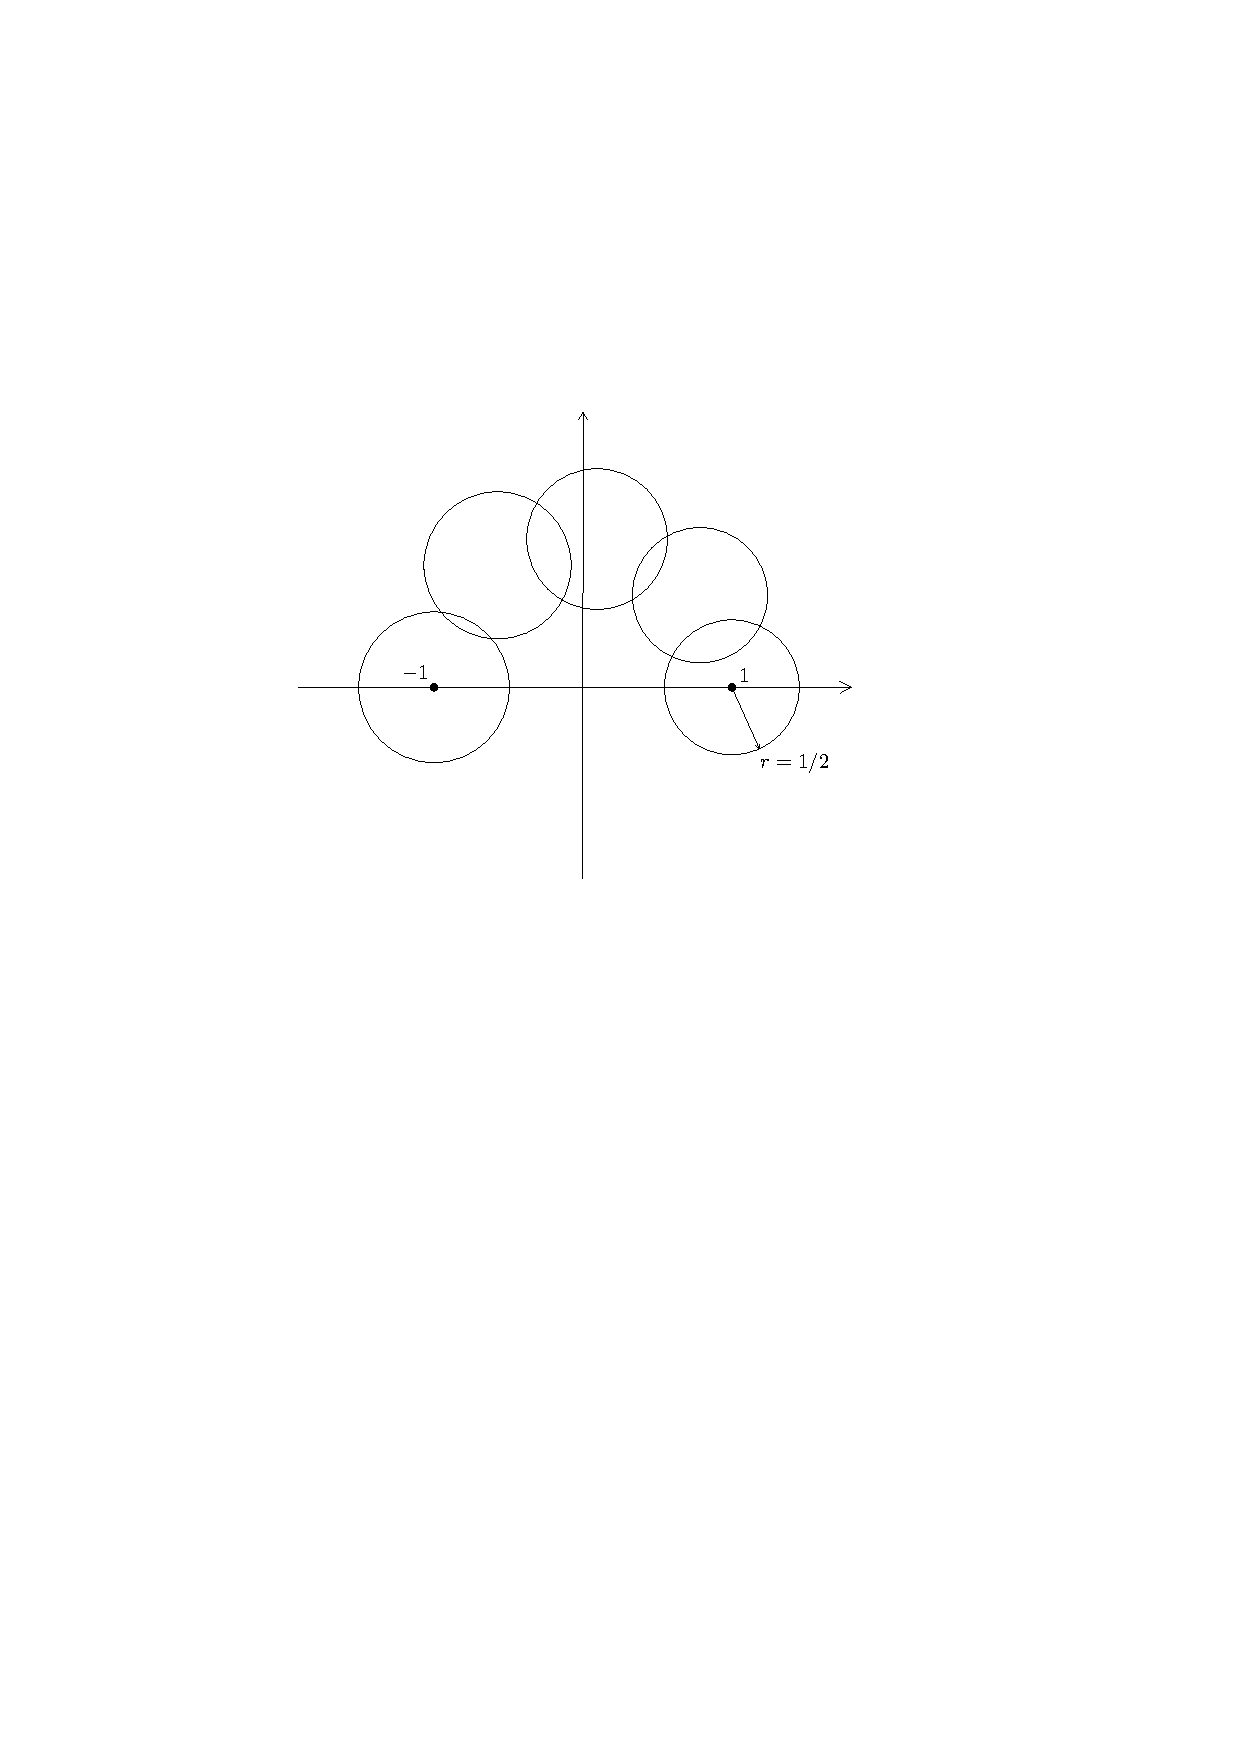
\includegraphics[width=180pt]{pictures/analytic-continuation-squreroot-1}
\end{figure}

However, we might have begun our analytic continuation process as shown below. If we continued the process to $z=-1$, we would have $f(-1)=-i$.
\begin{figure}[htbp]
\centering
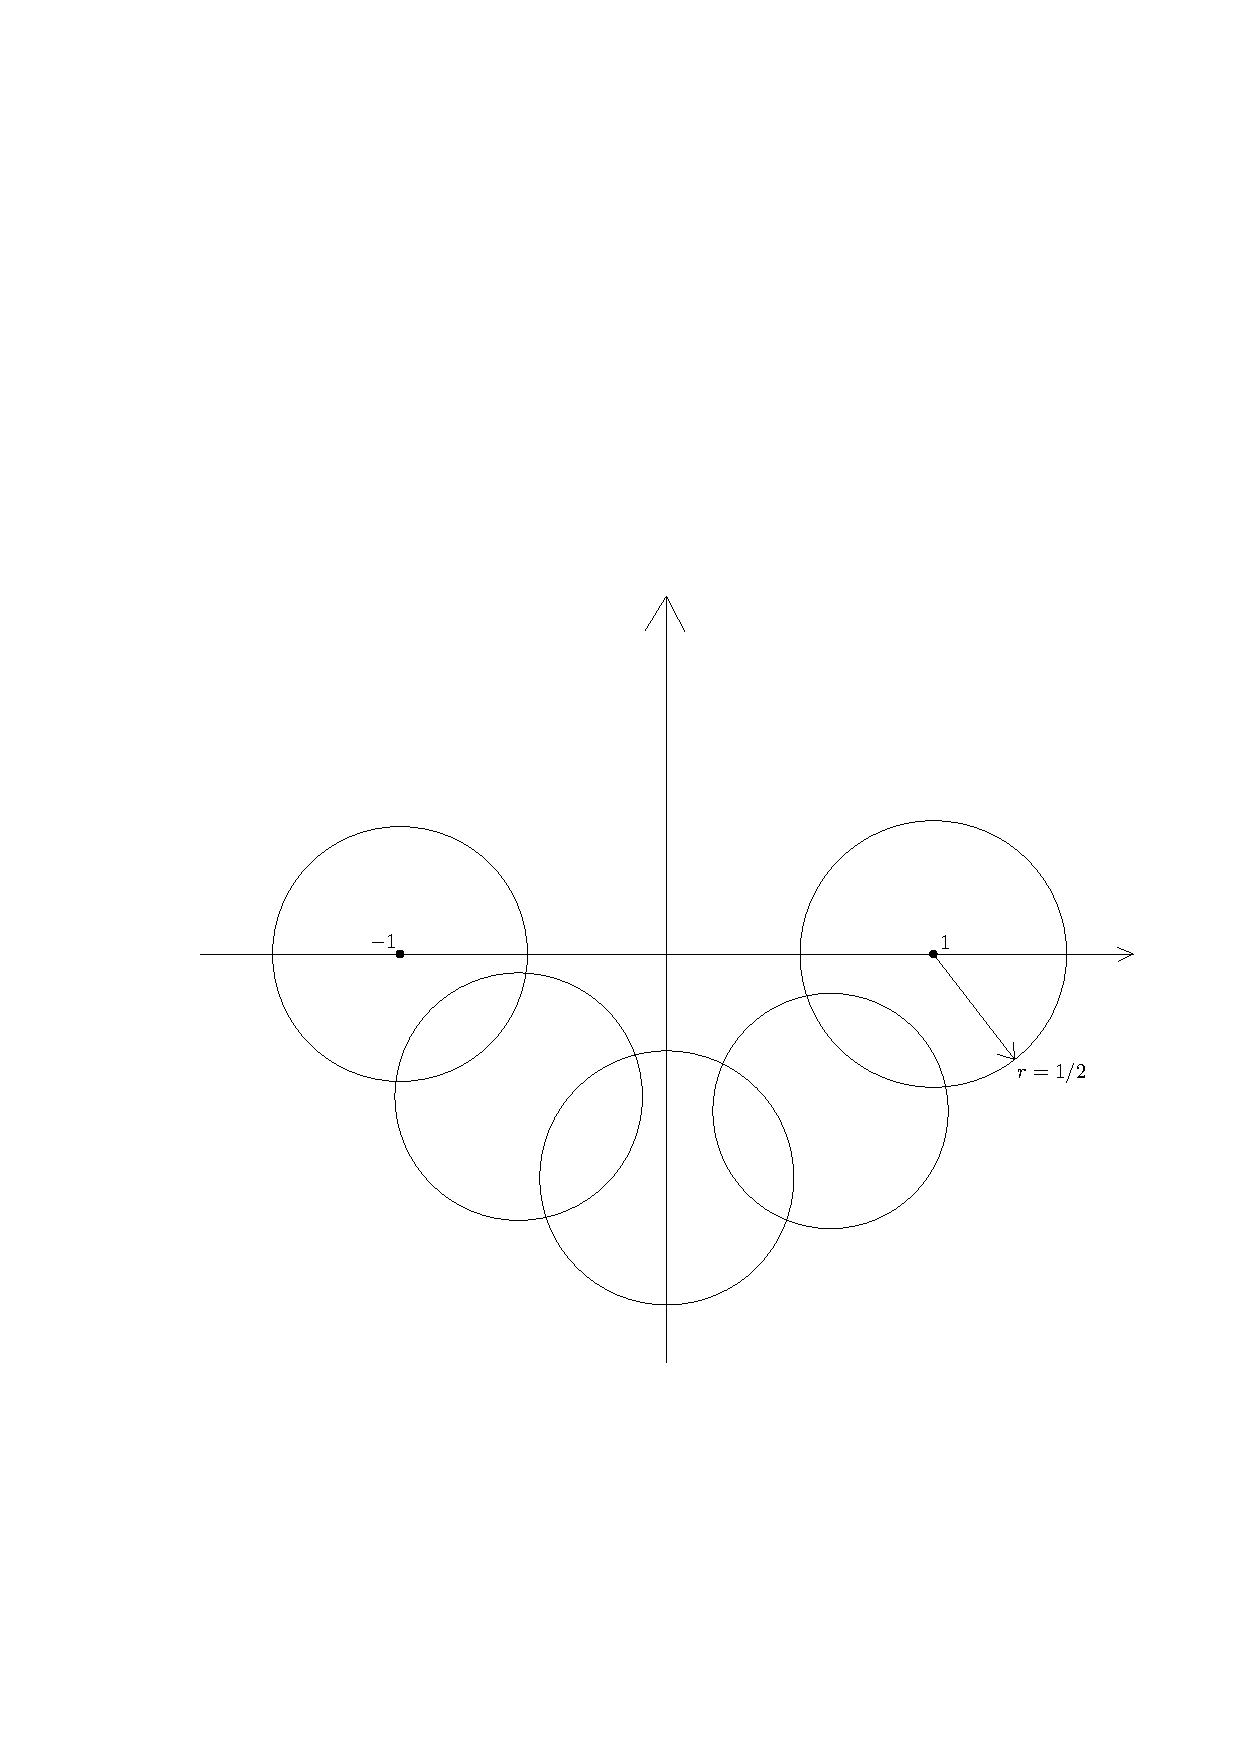
\includegraphics[width=180pt]{pictures/analytic-continuation-squreroot-2}
\end{figure}

Thus we see that the process of analytic continuation can be ambiguous. In the present example, the ambiguity is connected to the fact that a holomorphic square root function cannot be defined in any neighborhood of the origin.
\end{example}
These examples illustrate that an analytic function can sometimes be
continued to a domain of definition that is larger than the initial one. However, this continuation process can result in inconsistencies in the sense that the value of a continuation at a given point may depend on which continuation is involved, in effect, on how the point was reached. In each of the examples, the continuation process was effected differently by a device specific to the function. This raises two general and rather vague questions: How can we carry out analytic continuation in general? Furthermore, how can we determine when it can be carried out unambiguously? It is because of these questions that we must take a detailed and technical approach to the process of analytic continuation. Even making the questions themselves precise takes some thought.
\begin{definition}
A \textbf{function element} is an ordered pair $(f,U)$, where $U$ is a disc and $f$ is a holomorphic function defined on $U$.
\end{definition}
\begin{definition}
Let $(f,U)$ and $(g,V)$ be function elements. We say that $(g,V)$ is a \textbf{direct analytic continuation} of $(f,U)$ if $U\cap V\neq\emp$ and $f$ and $g$ are equal on $U\cap V$. Obviously $(g,V)$ is a direct analytic continuation of $(f,U)$ if and only if $(f,U)$ is a direct analytic continuation of $(g,V)$.
\end{definition}
If $(f_1,U_1),\dots,(f_k,U_k)$ are function elements and if each $(f_i,U_i)$ is a direct analytic continuation of $(f_{i-1},U_{i-1})$ for $i=2,\dots,k$, then we say that $(f_k,U_k)$ is an \textbf{analytic continuation} of $(f_1,U_1)$.\par
Clearly $(f_k,U_k)$ is an analytic continuation of $(f_1,U_1)$ if and only if $(f_1,U_1)$ is an analytic continuation of $(f_k,U_k)$. Also if $(f_k,U_k)$ is an analytic continuation of $(f_1,U_1)$ and $(f_{k+l},U_{k+l})$ is an analytic continuation of $(f_k,U_k)$ via a chain $(f_k,U_k),(f_{k+1},U_{k+1}),\dots,(f_{k+l},U_{k+l})$, then stringing the two chains together into $(f_1,U_1),\dots,(f_{k+l},U_{k+l})$ exhibits $(f_{k+l},U_{k+l})$ as an analytic continuation of $(f_1,U_1)$. Obviously $(f,U)$ is an analytic continuation of itself.\par
Thus we have an equivalence relation on the set of function elements.
The equivalence classes induced by this relation are called \textbf{(global) analytic functions}. However, a caution is in order: Global analytic functions are not yet functions in the usual sense, and they are not analytic in any sense that we have defined as yet. Justification for the terminology will appear in due course.\par
Notice that the initial element $(f,U)=(f_1,U_1)$ uniquely determines the global analytic function, or equivalence class, that contains it. But a global analytic function may include more than one function element of the form $(f,U)$ for a \textit{fixed disc} $U$. Indeed, a global analytic function $f$ may have in effect more than one value at a point of $\C$: Two function elements $(f_1,U)$ and $(f_2,U)$ can be equivalent even though $f_1(z_0)\neq f_2(z_0)$, where $z_0$ is the center of the disc $U$. If $\mathsf{f}$ denotes the global analytic function corresponding to $(f,U)$, then we call $(f,U)$ a branch of $\mathsf{f}$. Example~\ref{squre root continuation} illustrates a global analytic function (namely, the square root function) with two distinct branches centered at the point $-1$. Logarithms of $z$ again illustrate the point:
\begin{example}
Let $U=B_{1}(2)$ and let $f$ be the holomorphic function $\log z$. Here $\log z$ is understood to be defined as $\log|z|+i\arg z$, and $-\pi/6<\arg z<\pi/6$. As in the preceding example, the function element $(f,U)$ can be analytically continued to the point $-1$ in (at least) two different
ways, depending on whether the continuation is along a curve proceeding clockwise about the origin or counterclockwise about the origin.\par
In fact, all the branches of $\log z$ can be obtained by analytic continuation of the $\log|z|+i\arg z$ branch on $B_1(2)$.
\end{example}
In some situations, it is convenient to think of a function element as a convergent power series. Then the role of the open disc $U$ is played by the domain of convergence of the power series. This is a useful heuristic idea for the reader to bear in mind. From this viewpoint, two function elements $(f_1,U)$ and $(f_2,V)$ at a point $z_0$ (such that $U$ and $V$ are discs centered at the same point $z_0$) should be regarded as equal if $f_1=f_2$ on $U\cap V$. This identification is convenient and we shall introduce it formally a little later.
\subsection{Power series method of analytic continuation}
Now, we give an elegant and promising method of analytic continuation by means of power series. In this method, we use only circular domains and Taylor's expansion in such domain. Let the initial function $f_1(z)$ be represented by the Taylor's series about a point $z_1$ in the form
\begin{align}\label{power series continuation-1}
f_1(z)=\sum_{n=0}^{\infty}a_{n}^{(1)}(z-z_1)^n,
\end{align}
which converges within the circle $\Gamma_1:=\{z:|z-z_1|=\rho_1\}$. We now draw a path $\gamma$ from the point $z_1$ and perform the analytic continuation of the function along $L$ as follows: On $\gamma$, take a point $z_2$ such that the arc $z_1z_2$ lies in $\Gamma_1$, which is the circle of convergence of the series $(\ref{power series continuation-1})$. Then we use the series $(\ref{power series continuation-1})$ to evaluate the derivatives $f^{(n)}_1(z_2)$ by term-by-term differentiation and write the expansion which is valid within a circle $\Gamma_2:\{z:|z-z_2|=\rho_2\}$ in the form
\begin{align}\label{power series continuation-2}
f_2(z)=\sum_{n=0}^{\infty}a_{n}^{(1)}(z-z_2)^n=\sum_{n=0}^{\infty}\frac{f_2^{(n)}(z_2)}{n!}(z-z_2)^n.
\end{align}
If the circle $\Gamma_2$ extends beyond $\Gamma_1$, then $(\ref{power series continuation-2})$ gives an analytic continuation of $f_1(z)$. Also, at the point $z_2$, the functions $f_1(z)$ and $f_2(z)$ and all their derivatives have the same values. In this way, when the first analytic continuation of $(\ref{power series continuation-2})$ is performed, we proceed to the next.
\subsubsection{Singularities of power series on circles of convergence}
\begin{definition}
Let $f(z)$ be analytic in a domain $D$ and $F$ be the global analytic function determined by $f$. Let $\zeta$ be a point on $\partial D$. If no analytic continuation of $(z)$ to $\zeta$ is possible, then $\zeta$ is called a \textbf{singularity} of the global analytic function $F(z)$. If $\zeta\in\partial D$ is not a singularity, then it is called \textbf{regular}.
\end{definition}
\begin{theorem}
If the radius of convergence of the power series
\[f(z)=\sum_{n=0}^{\infty}a_nz^n\]
is nonzero finite, then $f(z)$ has at least one singularity on the circle of convergence.
\end{theorem}
\begin{proof}
Let $R$ be the radius of the circle of convergence $\Gamma$ of the power series and $D=B_{R}(0)$. Suppose, on the contrary, that every point of $\Gamma$ is a regular point of $f$. Then the compactness of $\Gamma$ implies then that there are open discs $D_1,\dots,D_n$ and functions $g_i\in\mathcal{H}(D_i)$ such that the center of each $D_i$ is on $\Gamma$, that $\Gamma\sub D_1\cup\cdots\cup D_n$, and that $g_i(z)=f(z)$ on $D_i\cap D$, for $i=1,\dots,n$.\par
If $D_i\cap D_j\neq\emp$ and $V_{ij}=D_i\cap D_j\cap D$, then $V_{ij}\neq\emp$ (since the centers of the $D_i$ are on $\Gamma$), and $g_i=f=g_j$ in $V_{ij}$. Since $D_i\cap D_j$ is connected, it follows that $g_i=g_i$ in $D_i\cap D_j$. Hence we may define a function $h$ in $\Omega:=D\cup D_1\cup\cdots\cup D_n$ by
\[h(z)=\begin{cases}
f(z)&z\in D,\\
g_i(z)&z\in D_i.
\end{cases}\]
Since $\widebar{D}\sub\Omega$ and $\Omega$ is open, there exists an $\eps>0$ such that the disc $B_{R+\eps}(0)\sub\Omega$. But $h\in\mathcal{H}(\Omega)$ and $h(z)=f(z)$ on $D$, so the radius of convergence of $f$ is at least $R+\eps$, contrary to our assumption.
\end{proof}
\subsubsection{The Hadamard gap theorem}
\begin{definition}
If a function $f(z)$ cannot be extended analytically beyond the boundary of a certain region $D$, then the boundary $\partial D$ is called a \textbf{natural boundary}.
\end{definition}
Now we present a technique of Ostrowski for producing series which exhibit a phenomenon called "over-convergence" (to be defined below). It was discovered by J.Hadamard that these series produce holomorphic
functions on the disc for which no point on $\partial\D$ is regular. The series are examples of what are called "gap series" (or "lacunary series"). These are series that are formed by deleting many terms from a series formed by a regular pattern. They have various uses in analysis. For instance, they can be used to construct continuous, nowhere differentiable functions.\par
Let us begin with a concrete example. Consider the power series $\sum_nz^{2^n}$. This series converges absolutely and uniformly on compact subsets of the unit disc $\D$ since $|z^{2^n}|\leq|z|^n$. Thus the power series defines a holomorphic function $f(z)$ on $\D$. We claim that no point of $\partial D$ is regular for $f$. To see this, consider $f(rw)$ for $0<r<1$ and $w$ such that $|w|^{2^N}=1$ for a fixed positive integer $N$. Now
\[f(rw)=\sum_{n=1}^{N-1}r^{2^n}w^{2^n}+\sum_{n=N}^{\infty}r^{2^n}w^{2^n}=\sum_{n=1}^{N-1}r^{2^n}w^{2^n}+\frac{1}{w}\sum_{n=N}^{\infty}r^{2^n}.\]
Thus we see $\lim_{r\to 1^-}|f(rw)|=+\infty$ since, for $N$ fixed, the first sum is bounded while the second tends to $+\infty$ (each summand is positive real and tends to a limit greater than $1$).\par
We conclude that $f'$ is unbounded near all $w\in\partial\D$ with $w^{2^N}=1$, some positive integer $N$. But the set of all such $w$ is dense in $\partial\D$, thus extension of $f$ to a neighborhood of a point in $\partial\D$ is impossible.\par
It is natural to try to generalize this example as much as possible. But the process is not easy. The proof of the following theorem uses a very clever trick, which at first might seem unmotivated. Try to see the elements of our example lurking in the background:
\begin{theorem}[\textbf{Ostrowski-Hadamard}]\label{Hadamard gap theorem}
Let $\{p_n\}$ be an increasing sequence of positive integers and suppose that there is a $\lambda>1$ such that
\[p_{n+1}>\lambda p_n\]
for all $n$. Suppose that, for some sequence of complex numbers $\{a_n\}$, the power series
\[f(z)=\sum_{n=0}^{\infty}a_nz^{p_n}\]
has radius of convergence $1$. Then no point of $\partial\D$ is regular for $f$.
\end{theorem}
\begin{proof}
Seeking a contradiction, we suppose that some $z_0\in\partial\D$ is regular for $f$; without loss of generality we take $z_0=1$. (This is indeed without loss of generality, since changing $z$ to $wz$, $|w|=1$, gives a series of the same form, with coefficients having the same absolute values as before; so the new series also has radius of convergence $1$.) Then there is a disc $B_{\eps}(1)$ and a holomorphic $F$ on $U=\D\cup B_{\eps}(1)$ extending $f$. Choose an integer $k>0$ such that $(k+1)/k<\lambda$ and define
\[\psi(z)=\frac{1}{2}(z^k+z^{k+1})\]
Notice that $\psi(1)=1$, and if $|z|\leq 1$ but $z\neq 1$, then we have
\[|\psi|=\frac{1}{2}|z|^k|z+1|<|z|^k\leq 1.\]
So $\psi(\D)$ is a compact subset of $U$. It follows by continuity of $\psi$ that there is a disc $B_{1+\delta}(0)$ such that $\psi(B_{1+\delta}(0))\sub U$. Note also that $1\in\psi(B_{1+\delta}(0))$.\par
Define
\[G(z)=F(\psi(z)),\quad z\in B_{1+\delta}(0)\]
and expand $G$ in a power series about $0$:
\[G(z)=\sum_{n=0}^{\infty}c_nz^n.\]
Compare this formula with what is obtained by substituting $\psi(z)=(z^k+z^{k+1})/2$ into the power series for $F=f$ on $\D$:
\[(F\circ\psi)(z)=\sum_{n=0}^{\infty}a_n\Big(\frac{z^k+z^{k+1}}{2}\Big)^{p_n}.\]
Notice that the $n$-th term of this series contributes powers of $z$ ranging from $z^{kp_n}$ to $z^{(k+1)p_n}$; while the $(n+1)$-st term contributes powers of $z$ ranging from $z^{kp_{n+1}}$ to $z^{(k+1)p_{n+1}}$. But the condition on $\{p_n\}$ and the choice of $k$ guarantees that $kp{n+1}>(k+1)p_n$, so that the powers appearing in $(z^k+z^{k+1})^{p_n}$ are pairwise disjoint. As a result, 
\[\sum_{n=0}^{N}a_n(\psi(z))^{p_n}=\sum_{n=0}^{(k+1)p_N}c_{n}z^n.\]
The right side converges as $N\to+\infty$ on the disc $B_{1+\delta}(0)$. Hence so does the left side. In other words,
\[\sum_{n=0}^{\infty}a_nw^{p_n}\]
converges for all $w\in\psi(B_{1+\delta}(0))$. In particular this series converges for all $w$ in a neighborhood of $1$, so its radius of convergence is not $1$. This contradicts our hypothesis.
\end{proof}
In general, a point $z_0$ in the boundary of the (unit) disc can be a regular point for the holomorphic function $f$ (on the disc) without the power series for $f$ about $0$ converging in a neighborhood of $z_0$. A good example is $f(z)=1/(1-z)$. Then all $z\in\partial\D\setminus\{1\}$ are regular but the radius of convergence of the power series is $1$. This explains why the phenomenon exhibited in the proof of Theorem~\ref{Hadamard gap theorem} is called \textbf{over-convergence}.\par
Now we return to the continuation of power series. We first show that, the singularities have close relation with the inconsistencies of continuation along curves.
\begin{theorem}
Suppose $D$ is a region, $L$ is a straight line or a circular arc, $D\setminus L$ is the union of two regions $D_1$ and $D_2$, $f$ is continuous in $D$, and $f$ is holomorphic in $D_1$ and in $D_2$. Then $f$ is holomorphic in $D$.
\end{theorem}
\begin{proof}
The use of linear fractional transformations shows that the general case follows if we prove the theorem for straight lines $L$. By Morera's theorem, it is enough to show that the integral of $f$ over the boundary $\partial R$ is $0$ for every rectangle $R$ with sides parallel to axis in $D$. The Cauchy theorem implies that the integral of $f$ vanishes over every closed path $\gamma$ in $R\cap D_1$ or in $R\cap D_2$. The continuity of $f$ shows that this is still true if part of $R$ is in $L$, and the integral over $\partial R$ is the sum of at most two terms of this sort.
\end{proof}
\subsection{Analytic continuation along a curve}
\begin{definition}
Let $(f,U)$ be a function element where $U$ is a region and $f$ is an analytic function in $U$. The \textbf{germ} of $f$ at $a$ is the collection of all function element $(g,V)$ such that $a\in V$ and $f(z)=g(z)$ for all $z$ in a neighborhood of $a$ and is denoted by $[f]_a$.
\end{definition}
Note that $[f]_a$ is a collection of function elements and it is not a function elements itself. Also, it can easily be verified that $(g,V)\in[f]_a$ if and only if $(f,U)\in[g]_a$, if and only if $f=g$ in a neighborhood of $a$.\par
We now revisit the definition of analytic continuation along a path in terms of germs as follows:
\begin{definition}
Let $(f,U)$ be a function element and let $\gamma:[0,1]\to\C$ be a path starting from $U$. Then an \textbf{analytic continuation of $\bm{(f,U)}$ along the curve $\bm{\gamma}$} is a collection $\{(f_t,U_t):t\in[0,1]\}$ such that
\begin{itemize}
\item[(a)] $(f_0,U_0)=(f,U)$.
\item[(b)] $\gamma(t)\in U_t$ for all $t\in[0,1]$.
\item[(c)] For each $t$ in $[0,1]$ there is a $\delta>0$ such that $|s-t|<\delta$ implies
\[\gamma(s)\in U_t\And[f_s]_{\gamma(s)}=[f_t]_{\gamma(t)}.\]
\end{itemize}
\end{definition}
\begin{theorem}\label{analytic continuation along curve unique}
Let $\gamma:[0,1]\to\C$ be a path from $z_0$ to $z_1$ and let $\{(f_t,U_t)\}$ and $\{(g_t,V_t)\}$ be analytic continuations along $\gamma$ such that $[f_0]_{z_0}=[g_0]_{z_0}$, then $[f_1]_{z_1}=[g_1]_{z_1}$.
\end{theorem}
\begin{proof}
In order to prove this claim we will show that the set
\[T=\{t\in[0,1]:[f_t]_{\gamma(t)}=[g_t]_{\gamma(t)}\}\]
is both open and closed in $[0,1]$. By hypotheses, we have $0\in T$, so $T$ is nonempty. Then it will follows that $T=[0,1]$ so that, in particular, $1\in T$.\par
To show that $T$ is open, fix $t$ in $T$ and assume that $t\neq 1$. In fact, if $t=1$ the proof is complete. By the definition of analytic, there is a $\delta>0$ such that for $|s-t|<\delta$, $\gamma(s)\in U_t\cap V_t$ and
\begin{align}\label{analytic continuation along curve unique-1}
[f_s]_{\gamma(s)}=[f_t]_{\gamma(t)},\quad [g_s]_{\gamma(s)}=[g_t]_{\gamma(t)}.
\end{align}
Since $t\in T$, it follows that $[f_t]_{\gamma(t)}=[g_t]_{\gamma(t)}$, so it follows that $[f_s]_{\gamma(s)}=[g_s]_{\gamma(s)}$ for $|s-t|<\delta$, therefore $(t-\delta,t+\delta)\sub T$. Therefore $T$ is open.\par
Next, to show that $T$ is closed let $t$ be a limit point of $T$, and again choose $\delta>0$ so that $\gamma(s)\in U_t\cap V_t$ and $(\ref{analytic continuation along curve unique-1})$ is satisfied whenever $|s-t|<\delta$. Since $t$ is a limit point of $T$, there is a point $s\in T$ with $|s-t|<\delta$, so
\[\gamma(s)\in U_t\cap U_s\cap V_t\cap V_s=:D.\]
Then $f_s(z)=g_s(z)$ on $D$ by the definition of $T$, and by $(\ref{analytic continuation along curve unique-1})$ we conclude that $[f_t]_{\gamma(t)}=[g_{t}]_{\gamma(t)}$, thus $t\in T$. This proves $T$ is closed.
\end{proof}
Thus we see that the analytic continuation of a given function element along a given curve is essentially unique, if it exists. From here on, to avoid being pedantic, we shall regard two analytic continuations $(f_t,U_t)$ and $(g_t,V_t)$ as "equal," or equivalent, if $[f_t]_{\gamma(t)}=[g_t]_{\gamma(t)}$ for all $t$. With this terminological convention (which will cause no trouble), the proposition says exactly that analytic continuation of a given function element along a given curve is unique. It should be stressed, however, that this is a uniqueness statement only-not an existence statement.
\subsection{Monodromy theorem and its consequences}
Let $z_0$ and $z_1$ be two points in $\C$ and suppose $\gamma$ and $\sigma$ are two paths from $z_0$ to $z_1$. Suppose that $\{(f_t,U_t)\}$ and $\{(g_t,V_t)\}$ are analytic continuations along $\gamma$ and $\sigma$, respectively. Also, suppose that $[f_0]_{z_0}=[g_0]_{z_0}$. 

According to Proposition~\ref{analytic continuation along curve unique} that the answer to this question is affirmative, if $\gamma$ and $\sigma$ are the same path. However, if $\gamma$ and $\sigma$ are distinct paths then the answer may be negative.\par
If $(f,D)$ is a function element and $z_0\in D$ then $f$ has a power series expansion at $z=z_0$. To establish the Monodromy theorem, our first step will be to investigate the behavior of the radius of convergence for an analytic continuation along a curve.
\begin{lemma}\label{analytic continuation along curve convergent radius}
Let $\gamma:[0,1]\to\C$ be a path and let $\{(f_t,U_t)\}$ be an analytic continuation along $\gamma$. For $t\in[0,1]$, let $R(t)$ be the radius of convergence of the power series expansion of $f_t$ about $z=\gamma(t)$. Then either $R(t)\equiv+\infty$ or $R:[0,1]\to(0,+\infty)$ is continuous.
\end{lemma}
\begin{proof}
If $R(t)=+\infty$ for some value of $t_0$; that is, the radius of circle of convergence is infinite. Then it is possible to extend $f_{t_0}$ to an entire function. If we consider another analytic continuation along $\gamma$ defined by $\{\widetilde{f}_t=f_{t_0},V_t=\C)\}$, then by Proposition~\ref{analytic continuation along curve convergent radius} we have $[f_t]_{\gamma(t)}=[\widetilde{f}_t]_{\gamma(t)}=[f_{t_0}]_{\gamma(t)}$. This implies $f_s=f_{t_0}$ on $U_t$, and therefore each $f_t$ can be extended to an entire function. Thus $R(t)\equiv+\infty$.\par
So we suppose that $R(t)<+\infty$ for all $t\in[0,1]$. Fix $t_0$ in $[0,1]$ and let $z_0=\gamma(t_0)$. Let the power series expansion of $f_{t_0}$ about $z_0$ be
\[f_{t_0}(z)=\sum_{n=0}^{\infty}a_n(z-z_0)^n\]
Now let $\delta_1>0$ be such that $|s-t_0|<\delta_1$ implies
\[\gamma(s)\in U_{t_0}\cap B_{R(t_0)}(z_0)\And [f_s]_{\gamma(s)}=[f_{t_0}]_{\gamma(t_0)}.\]
Let us fix $s$ with $|s-t_0|<\delta_1$. Now we can extend $f_{t_0}$ to an analytic function in $B_{R(t_0)}(z_0)$. Again, since $f_s$ agree with $f_{t_0}$ on a neighborhood of $\gamma(s)$, $f_s$ can be extended. Consequently, $f_s$ is also analytic in $B_{R(t_0)}(z_0)\cup U_s$. Suppose $f_s$ has the power series expansion about $\gamma(s)$ as
\[f_s(z)=\sum_{n=0}^{\infty}b_n(z-\gamma(s))^n\]
then the radius of convergence $R(s)$ must be at least as big as the distance from $\gamma(s)$ to the circle $\Gamma_0=\{z:|z-z_0|=R(t_0)\}$; that is,
\[R(s)\geq d(w,\Gamma_0)=R(t_0)-|z_0-\gamma(s)|.\]
This implies
\[R(t_0)-R(s)\leq|z_0-\gamma(s)|.\]
By symmetric, we can establish the other direction, and hence we have
\[|R(t_0)-R(s)|\leq|z_0-\gamma(s)|.\]
Since $\gamma$ is a continuous function, this inequality then implies $R$ is continuous.
\end{proof}
\begin{lemma}\label{analytic continuation along curve small pertubation}
Let $\gamma:[0,1]\to\C$ be a path from $z_0$ to $z_1$ and let $\{(f_t,U_t)\}$ be an analytic continuation along $\gamma$. There is a number $\eps>0$ such that if $\sigma:[0,1]\to\C$ is any path from $z_0$ to $z_1$ with $|\gamma(t)-\sigma(t)|<\eps$ for all $t$ and if $\{(g_t,V_t)\}$ is any continuation along $\sigma$ with $[g_0]_{z_0}=[f_0]_{z_0}$, then $[g_1]_{z_1}=[g_1]_{z_1}$.
\end{lemma}
\begin{proof}
Let power series expansion of $f_t$ about $\gamma(t)$ be
\[f_t(z)=\sum_{n=0}^{\infty}a_n(z-\gamma(t))^n.\]
and let $R(t)$ be its radius of convergence. If $R(t)\equiv+\infty$, then any value of $\eps$ will serve our purpose. So suppose $R(t)<+\infty$. Since, by the preceding Lemma, $R(t)$ is a continuous function and since $R(t)>0$ for all $t$, $R(t)$ has positive minimum value $m$. Let $0<\eps<m/2$. Suppose that $\sigma$ and $\{(g_t,V_t)\}$ are as in the statement of this lemma. Also, suppose that $U_t$ is the disk given by $U_t=\{z:|z-\gamma(t)|<R(t)\}$. This supposition will not affect the conclusion of the lemma.\par
Since, for $\sigma(t)\in U_t\cap V_t$ and for all $t\in[0,1]$, we have $|\sigma(t)-\gamma(t)|<\eps<R(t)$, it makes sense to ask whether $g_t(z)=f_t (z)$ for all $z$ in $U_t\cap V_t$. In order to complete the proof, we will show that this is precisely the case. Define the set $T$ by
\[T=\{t\in[0,1]:f_t(z)=g_t(z)\text{ for }z\in U_t\cap V_t\}.\]
We will show that $T$ is open and closed. Since $0\in T$, this will implies $T=[0,1]$ and completes the proof.\par
By hypothesis of the lemma, $[f_0]_{z_0}=[g_0]_{z_0}$; it follows that $f_0(z)=g_0(z)$ for $z\in U_t\cap V_t$ and so $0\in T$. Thus $T\neq\emp$. To show that $T$ is open, let us fix $t\in T$ and choose $\delta>0$ such that $|s-t|<\delta$ implies that
\begin{align}\label{analytic continuation along curve small pertubation-1}
\gamma(s)\in U_t,|\gamma(s)-\gamma(t)|<\eps,[f_s]_{\gamma(s)}=[f_t]_{\gamma(t)}
\end{align}
and
\begin{align}\label{analytic continuation along curve small pertubation-2}
\sigma(s)\in V_t,|\sigma(s)-\sigma(t)|<\eps,[f_s]_{\sigma(s)}=[f_t]_{\sigma(t)}.
\end{align}
We now show that $U_t\cap U_s\cap V_t\cap V_s\neq\emp$ for $|s-t|<\delta$. This will be proved by showing that $\sigma(s)\in U_t\cap U_s\cap V_t\cap V_s$. If $|s-t|<\delta$, then
\[|\sigma(s)-\gamma(s)|<\eps<R(s)\]
and thus $\sigma(s)\in U_s$. Also,
\[|\sigma(s)-\gamma(t)|\leq|\sigma(s)-\gamma(s)|+|\gamma(s)-\gamma(t)|<\eps+\eps<R(t)\]
so $\sigma(s)\in U_t$. We already have that $\sigma(s)\in V_s\cap V_t$, so we conclude that $\sigma(s)\in D:=U_t\cap U_s\cap V_t\cap V_s$. Again, since $t\in T$ it follows that $f_t(z)=g_t(z)$ for $z\in D$, and by $(\ref{analytic continuation along curve small pertubation-1})$ and $(\ref{analytic continuation along curve small pertubation-2})$ we conclude that $f_s(z)=g_s(z)$ for all $z\in D$. But since $D$ has a limit point in $U_s\cap V_s$ it must follows that $s\in T$; that is, $T$ is open. One can easily show that $T$ is closed. This completes that proof of the lemma.
\end{proof}
\begin{definition}
Let $(f,U)$ be a function element and let $D$ be a region which contains $U$; then $(f,U)$ \textbf{admits unrestricted analytic continuation in $\bm{D}$} if for any path $\gamma$ in $D$ with initial point in $U$, there is an analytic continuation of $(f,U)$ along $\gamma$.
\end{definition}
Let us consider $U=B_{1}(1)$ and $f$ be the principal branch of $\sqrt{z}$ or $\log z$. Then we see that $(f,U)$ admits unrestricted continuation in the punctured plane but not in the whole plane.\par
It may remarkable that if $(f,U)$ is a function element and $D$ is a region containing $U$, no criterion will be given which implies that $(f,U)$ admits unrestricted continuation in $D$. In fact, the Monodromy Theorem assumes that $D$ has this propriety and states a uniqueness criterion.
\begin{theorem}[\textbf{Monodromy Theorem}]\label{Monodromy Theorem}
Let $(f,U)$ be a function element and let $D$ be a region containing $U$ such that $(f,U)$ admits unrestricted continuation in $D$. Let $z_0\in U$, $z_1\in D$ and let $\gamma_0$ and $\gamma_1$ be paths in $D$ from $z_0$ to $z_1$. Let $\{(f_t,U_t)\}$ and $\{(g_t,V_t)\}$ be analytic continuation of $(f,U)$ analog $\gamma_0$ and $\gamma_1$, respectively. If $\gamma_0$ and $\gamma_1$ are homotopic in $D$, then $[f_1]_{z_1}=[g_1]_{z_1}$.
\end{theorem}
\begin{proof}
Let $H:[0,1]^2\to D$ be a homotopy between $\gamma_0$ and $\gamma_1$. Consider the path $\gamma_u$ defined by
\[\gamma_u=H(t,u)\]
Again, by hypothesis, there is a analytic continuation $\{(h_{(t,u)},D_{(t, u)})\}$ along the path $\gamma_u$. Form Proposition~\ref{analytic continuation along curve unique} of the preceding section, it follows that $[g_1]_{z_1}=[h_{1,1}]_{z_1}$ and $[f_1]_{z_1}=[h_{1,0}]_{z_1}$. Hence, it is sufficient to show that $[h_{1,0}]_{z_1}=[h_{1,1}]_{z_1}$.\par
We now introduce the set
\[U=\{u\in[0,1]:[h_{1,u}]_{z_1}=[h_{1,0}]_{z_1}\}.\]
and we will show that $U$ is a nonempty open and closed subset of $[0,1]$. Evidently, $0\in U$, so $U$ is nonempty. For a fixed $u$ in $[0,1]$, apply Lemma~\ref{analytic continuation along curve small pertubation} to find an $\eps>0$ that satisfies the condition in the lemma for $\gamma_u$. Now since $H$ is a uniformly continuous function, it follows that for any given $\eps>0$, there exists $\delta>0$ such that
\begin{align}\label{Monodromy Theorem-1}
|u-v|<\delta\Longrightarrow|\gamma_u(t)-\gamma_v(t)|<\eps\text{ for all $t$}\Longrightarrow[h_{1,u}]_{z_1}=[h_{1,v}]_{z_1}.
\end{align}
Now by the assumption on $\eps$, we conclude $[h_{1,v}]_{z_1}=[h_{1,0}]_{z_1}$ provided $|u-v|<\delta$. This implies $U$ is an open set.\par
If $u$ is a limit point of $U$ and $\delta>0$ is chosen such that $(\ref{Monodromy Theorem-1})$ holds. Then there exists a $v\in U$ such that $|u-v|<\delta$. But by $(\ref{Monodromy Theorem-1})$ and the definition of $U$,
\[[h_{1,u}]_{z_1}=[h_{1,v}]_{z_1}=[h_{1,0}]_{z_1}.\]
Thus $u\in U$. Hence $U$ is closed, and the proof is completed.
\end{proof}
Observe that the following corollary is the most important consequence of the Monodromy Theorem.
\begin{corollary}
Let $(f,U)$ be a function element which admits unrestricted continuation in the simply connected region $D$. Then there is an analytic function $F:D\to\C$ such that $F(z)=f(z)$ for all $z$ in $U$.
\end{corollary}
\begin{proof}
Let us chosen a point $z_0$ in $U$ and keep it fix and let $z$ be any point in $D$. Let $\gamma$ be a path in $D$ from $z_0$ to $z$ and $\{(f_t,U_t)\}$ be an analytic continuation of $(f,U)$ along $\gamma$; then let $F(z)=f_t(z)$. Since $D$ is simply connected, the value of $F$ does not depend on the choice of $\gamma$, so $F$ is well-defined on $D$. Since $F$ equals to an analytic function near every point of $D$, it follows that $F$ is analytic. It is clear that $F(z)=f(z)$ on $U$.
\end{proof}